\documentclass[11pt,a4paper]{article}
\usepackage{amsmath,amssymb,amsthm}
\usepackage[margin=2.5cm]{geometry}
\usepackage{graphicx}
\usepackage{xcolor}
\usepackage{booktabs}
\usepackage{tabularx}
\usepackage{longtable}
\usepackage[export]{adjustbox}
\usepackage{enumitem}
\usepackage{microtype}
\usepackage{needspace}
\usepackage[section]{placeins}
\usepackage[colorlinks=true,linkcolor=blue!55!black,citecolor=blue!55!black,
            urlcolor=blue!55!black,bookmarks=true,bookmarksnumbered=true,
            unicode=true]{hyperref}

\widowpenalty=10000
\clubpenalty=10000

\theoremstyle{plain}
\newtheorem{theorem}{Theorem}[section]
\newtheorem{lemma}[theorem]{Lemma}
\newtheorem{corollary}[theorem]{Corollary}
\newtheorem{proposition}[theorem]{Proposition}
\newtheorem{conjecture}[theorem]{Conjecture}
\theoremstyle{definition}
\newtheorem{definition}[theorem]{Definition}
\newtheorem{example}[theorem]{Example}
\theoremstyle{remark}
\newtheorem{remark}[theorem]{Remark}

\newcommand{\Z}{\mathbb{Z}}
\newcommand{\R}{\mathbb{R}}
\newcommand{\T}{\mathbb{T}}
\newcommand{\floor}[1]{\left\lfloor #1 \right\rfloor}
\newcommand{\wn}[1]{\lVert #1 \rVert_{N}}
\newcommand{\wnc}[1]{\lVert #1 \rVert}
\DeclareMathOperator{\ord}{ord}
\DeclareMathOperator{\cls}{cls}

\graphicspath{{.}}

\hypersetup{
  pdftitle={The Lonely Runner Problem on Pair-Sum Lattices: A Lossless
            Finitization and a Conditional Scaling-Closure Theorem for the
            Covering Obstruction (v3)},
  pdfauthor={Anonymous},
  pdfsubject={Lonely Runner Conjecture; Diophantine approximation;
              cyclic covering; combinatorics},
  pdfkeywords={Lonely Runner Conjecture, pair-sum lattice, finitization,
               covering systems, rigid zone, translate classes, group ring,
               cyclotomic, tensor translation, higher rungs, fiber cascade,
               conditional theorem, hypothesis ledger}
}

\begin{document}

\tableofcontents
\newpage

% ======================================================================
% Section 1 — Introduction
% ======================================================================

\begin{abstract}
\noindent
We prove an exact identity that reduces the maximum loneliness of a Lonely
Runner instance to a finite maximum over cyclic groups: for every speed
vector $V$ of $n$ positive integers,
$M(V)=\max_{\{u,w\}}\tau(u,w)$, where $\tau(u,w)$ is the optimal loneliness
on the pair-sum lattice of denominator $N=v_u+v_w$. The analytic core of the
argument is folklore (it appears in a comment on Tao's 2015 blog post); the
contributions claimed here are the sharpening that sum lattices alone always
suffice, the exact equality, and the lossless reformulation of the Lonely
Runner Conjecture ($\mathrm{LRC}$-$_n$) as the finite statement
$(\mathrm{TAU}$-$_n)$. The reformulation turns the conjecture into a family
of covering problems: a pair certifies iff $n-1$ explicit bad sets
$B_w=\{k\in\Z_N : (n{+}1)\,\wn{wk}<N\}$ fail to cover $\Z_N$. We develop
this covering geometry: an exact size law, a class-group reduction at prime
moduli, a lift law, and complete classifications of the unit coverings at
the prime moduli $7,11,13$ (three bad sets) and $7,13,17,19,37$ (four bad
sets)---at every such prime, covering is governed by a short explicit list
of translate classes in a cyclic group. Empirically, these five primes form
the entire unit-capable \emph{rigid zone} at $n=5$ within the verified range
(primes $\le 150$, composites $\le 111$), a striking but unproved finiteness
statement. On the full corpus of $3{,}712{,}576$ primitive speed sets with
$n=5$ and speeds $\le 56$, proved lemmas close $75.6\%$ of instances
($78.2\%$ including a coincidence-counting lemma), per-modulus verification
closes all of them, and the residual obstruction is localized to a single
named class (mixed order signatures at composite moduli). The proved-coverage
rate declines as the corpus grows ($93.4\%\to78.2\%$ over $V=24\to56$ on the
augmented battery, crossing below the continuation threshold at $V=56$);
the trend does not establish that coverage stabilizes, and its asymptotics
are unresolved. We report the decline, the localization, and the exact
verification record as the paper's empirical findings.
The paper's culminating result is stated as a \emph{conditional}
theorem (Theorem~\ref{thm:SC}): under three named open hypotheses---the
multi-fiber survivor inequality Hq (quantified in this revision; it
subsumes the former dilate-sparsity input H2m as its one-step case),
the distinct-family volume law H1g with its uniform margin, and the
resonance budget H2r---the fiber cascade closes the covering
obstruction at the frontier cells $(1K,T{-}3U)$ of every rung $T\ge 8$
at $N=p^2$ within a depth that is $T$-flat in practice and never
exceeds $T+3$ in the worst case. The reduction chain and every other
input (normal form, reflection fiber, chain-class theorem,
renormalization lemma, lossless equivalence) are proved or
machine-validated, and each constant's provenance---derived, measured,
or fitted, with the data it is fit to---is disclosed in the hypothesis
ledger.
That boundary between the proved and the hypothesized has a structural
type, verified statement-by-statement in \S\ref{sec:scale-status}: every
proved result in this program is a closure, invariance, exhaustiveness,
or machine-verification statement, while every remaining obligation is a
uniform growth-in-$k$ margin over a trivial or measured baseline---a
statement type no turn of the program has proved. This type mismatch is
why the paper stops where it stops. The one candidate instrument
shaped to produce that missing type was a transfer-matrix or automaton
model of the strand census. It was executed as a proof attempt under a
pre-committed success criterion and closed by theorem (for automata
built on the cascade's bijective drift)
(Lemma~\ref{lem:monomial}). The cascade's constrained transfer
matrices are partial permutations with a spectral radius of exactly $0$
or $1$ at every scale. The cyclic product is diagonal, with trace equal
to the survivor count itself, and the missing margin is provably
external to the lossless dynamics. The reformulation is bounded by its
own fidelity: the losslessness that makes it a faithful rewrite is the
property that withholds the decay a margin would require.
This is a structural paper: it does not solve or reduce the Lonely
Runner Conjecture, proves no new cases of it, and claims nothing beyond
the verified ranges stated in the text; the two hypotheses of
Theorem~\ref{thm:SC} are open and are not silently established anywhere.
\end{abstract}

\section{Introduction}\label{sec:intro}

\subsection{The conjecture and its status}

Let $n\ge 2$ and let $V=(v_1,\dots,v_n)$ be distinct positive integer
speeds. Runners start together at the origin of the unit circle
$\T=\R/\Z$ at time $0$; runner $p$ occupies $v_p t \bmod 1$ at time $t$.
Write $\wnc{x}$ for the distance of a real number to the nearest integer.
The \emph{loneliness} of the stationary observer (runner $0$) at time $t$
is
\[
g(t)\;=\;\min_{1\le p\le n}\;\wnc{v_p t},
\qquad
M(V)\;=\;\max_{t\in\T}\,g(t).
\]
The Lonely Runner Conjecture ($\mathrm{LRC}$-$_n$), posed by Wills in 1967
and independently by Cusick in the language of view obstruction
\cite{PS-survey,Wills,Cusick1973}, asserts $M(V)\ge 1/(n{+}1)$ for every $V$ with
$\gcd(V)=1$; by translation symmetry this is the statement that every
runner on the track becomes lonely at some time. The conjecture is known
for at most seven runners (Bohman--Bohman--Holzman and
Barajas--Serra; see the survey \cite{PS-survey} for history and precise
references). The frontier has since moved entirely into computer-assisted
territory: eight runners \cite{Rosenfeld8}, nine and ten runners
\cite{Trakulthongchai}, eleven through thirteen runners
\cite{Sungkawichai}, and fourteen and fifteen runners \cite{Allikvere},
the last with public certificates, resting on the linearly-exponential
checking bounds of Malikiosis--Santos--Schymura \cite{MSS}.

Two neighboring literatures study the fine structure of the problem rather
than new rungs. The \emph{spectrum} line computes exact optimal values
$\mathrm{ML}=p/q$ and their denominators
\cite{Kravitz,FanSun,GiriKravitz,Cordella}, including tight-instance
classifications \cite{Zhang}. The \emph{relations} line localizes
counterexamples and tight instances to low-weight integer hyperplanes in
parameter space \cite{BeckEverett}. The closest formulation in spirit is
Rifford's \cite{Rifford}: he studies the \emph{time} it takes a runner to
become lonely, shows that bounding that time by a number of rounds is
equivalent to a covering problem in dimension $n-2$ on the continuous torus,
formulates a covering conjecture there and proves it for $n\le 6$, and
bounds the one-round gap of loneliness by $1/(2m-1)$. What the two
formulations share is the move from runners to coverings; what separates
them is the domain and the mode. Rifford's covering problem is continuous
and its conjecture is a sufficient condition for a time bound, while the
present reduction is finite and exact---an identity, not an
inequality---reducing the threshold question itself to coverings of the
cyclic groups $\Z_{v_u+v_w}$ by multiplicative bad sets. That finiteness is
what makes the arithmetic visible: nothing corresponding to the rigid zone,
the translate-class classifications, or the kernel world appears in, or is
excluded by, the continuous formulation, and none of our results overlap
his. The present paper is a reformulation paper whose subject is the
geometry of the obstruction itself, at small moduli, in residue language.

\subsection{What this paper does}

The starting point is a classical observation: the optimal time is rational,
and its denominator is the sum or difference of two speeds. In the form
relevant here---``the maximum is attained at an intersection of two sine
curves, so the optimal time is rational with denominator the sum or
difference of two integer velocities''---this appears in a comment on Tao's
blog post of 13 May 2015 \cite{Tao-blog}. We treat that technique as known
folklore and cite it as such. What the folklore does not record, and what
this paper builds on, is the following sharpening and its consequences.

\begin{enumerate}[leftmargin=1.6em,itemsep=2pt]
\item \textbf{The sum-only equality theorem}
  (\S\ref{sec:equality}). At a global optimum with $0<M<\tfrac12$ the
  binding runners can be chosen two-sided, which forces the optimal time
  onto the lattice of a \emph{sum} $v_u+v_w$; difference denominators never
  carry the optimum. On that lattice the two binding runners are exact
  reflections of each other at \emph{every} lattice time
  (Lemma~\ref{lem:mirror}), so the $n$-runner minimum there equals an
  $(n{-}1)$-runner minimum. Together these give the exact identity
  $M(V)=\max_{\{u,w\}}\tau(u,w)$ of Theorem~\ref{thm:equality}---not an
  inequality---and the lossless equivalence of
  Corollary~\ref{cor:tau}: $\mathrm{LRC}$-$_n$ holds iff
  $(\mathrm{TAU}$-$_n)$ does, a \emph{finite} statement about explicit
  cyclic groups $\Z_{v_u+v_w}$. The finitization is exact: no information
  is lost, and nothing about the classical difficulty of the conjecture is
  claimed to become easier.
\item \textbf{The covering framework} (\S\ref{sec:covering}). Pair
  certification becomes a covering question: a pair fails iff its $n-1$ bad
  sets $B_w=\{k : (n{+}1)\wn{wk}<N\}$ cover $\Z_N$. Five empirically
  distinct obstruction classes from the program's earlier experiments
  collapse into \emph{additive orders of one covering phenomenon}
  (Table~\ref{tab:taxonomy}). The framework yields proved lemmas: an exact
  size law (Lemma~\ref{lem:size}), a polygonal witness lemma
  (Lemma~\ref{lem:jgon}), moat counting (Lemma~\ref{lem:counting}), a
  coincidence-counting lemma (Lemma~\ref{lem:D3}), a lift law
  (Lemma~\ref{lem:lift}), and a class-group reduction at prime moduli
  (Lemma~\ref{lem:class}).
\item \textbf{The rigid zone and its classifications}
  (\S\ref{sec:rigid}). At each rung $n$ there is a small set of
  \emph{unit-capable} moduli---those $N$ for which $n-1$ unit bad sets can
  cover $\Z_N$: $\{7,11,13\}$ at $n=4$ and $\{7,13,17,19,37\}$ at $n=5$
  within the verified range. We classify the covering configurations
  completely at every one of these primes
  (Theorems~\ref{thm:K4}--\ref{thm:K37}): each classification is a short
  explicit list of translate classes in a cyclic group (antipodal classes,
  domino tilings, perfect matchings, and at $19$ and $37$ the two classes
  $\{0,1,2,7\}$, $\{0,2,4,6\}$ and the single class $\{0,2,12,15\}$).
  This is the paper's central structural finding: \emph{at rigid primes,
  the covering obstruction is governed by a small translate-class
  structure}. The measured coverage rates of \S\ref{sec:measure} are a
  consequence of this structure, not the primary result.
\item \textbf{The measurement} (\S\ref{sec:measure}). On all
  $3{,}712{,}576$ primitive $5$-sets with speeds $\le 56$: proved lemmas
  close $75.6\%$ ($78.2\%$ with the coincidence lemma), per-modulus
  verification closes $100\%$, and every set has a certifying pair at a
  never-covering configuration. The proved-coverage rate declines as the
  corpus grows ($93.4\%\to78.2\%$ over $V=24\to56$ on the augmented
  battery, crossing below the continuation threshold at $V=56$); the trend
  does not establish stabilization, and the decline is reported as a
  finding, with the residual localized to one named class (mixed order
  signatures at composite moduli).
\item \textbf{The conditional scaling-closure theorem}
  (\S\ref{sec:SC}, \S\ref{sec:scale}). The frontier cells
  $(1K,T{-}3U)$ at $N=p^2$---beyond the reach of enumeration---are
  attacked structurally: the fiber cascade of \S\ref{sec:higherrung}
  reduces, exactly, to iterated dilate-intersections of census solution
  sets (Lemma~\ref{lem:twofiber}), and the closure question becomes a
  pool-versus-cut arithmetic. What is proved: the pool law, the spacing
  lemma, the $k$-cancellation, the free reflection fiber
  (Lemma~\ref{lem:reflect}), the chain-class dilate theorem
  (Theorem~\ref{thm:chaindilate}), and the renormalization lemma
  (Lemma~\ref{lem:renorm}). What is measured: the pool saturation at two
  rungs (the $840$ identity is a $p=17$ accident, disclosed as such),
  the zone-resolved cut quality, and the $T=8$ volume law with margin
  growing in $k$. What remains is consolidated into \emph{one} named
  conditional theorem (Theorem~\ref{thm:SC}) with a six-entry hypothesis
  ledger, a free-parameter disclosure ($c_1$ data-bounded, $\Lambda_0\approx4$
  data-chosen, $\gamma_0$ data-bounded, the fitted $R$ retired), and
  sampled estimates carrying their intervals and \emph{projected} labels.
  The two open obligations are reduced to named objects: the strand
  census (for H1g) and the sharp pair-line constants (for H2m).
  The boundary between those two lists has a structural type, and it
  explains where the paper stops: every proved result in the
  program---everything enumerated above and everything in the sections
  that follow---is a closure, invariance, exhaustiveness, or
  machine-verification statement, while every remaining obligation (the
  H1g margin over the trivial bound, the volume law's growth in $k$, the
  chain class's gap from measured to proved constants) is a uniform
  growth-in-$k$ margin over a trivial or measured baseline. No turn of
  the program has proved a statement of the second type; the audit of
  \S\ref{sec:scale-status} verifies this statement-by-statement,
  including the one candidate that reads like an exception, the cut
  law's ``$k$-cancellation,'' which cancels the $k$-dependence---a
  $k$-invariance, the exact opposite of a growth-in-$k$ margin. The
  empirical half of the reading is thereby settled; the structural half
  (that a classification toolkit cannot produce the missing type) is a
  hypothesis about tool reach. If it is right, the reformulation cannot
  close the conjecture in its current form: it closes the covering
  obstruction exactly where classification suffices, and the residual is
  a growth-in-$k$ margin of a type that has resisted every census-shaped
  attack the program has tried---a structural gap, not a technical one.
  The one margin-shaped candidate was then executed as a proof attempt
  on the committed cells under a pre-committed success criterion
  ($\rho\le 1-\epsilon$, $\epsilon$ independent of $k$), with the state
  space and the whole-cascade comparison target fixed beforehand. It
  closed by theorem for the lossless state space, not by measurement:
  the constrained transfer
  matrices of the lossless cascade are partial permutations
(Lemma~\ref{lem:monomial}), every spectral quantity in the framework
is exactly $0$ or $1$, the cyclic product is diagonal---its trace is
the cascade's own survivor count---and the survival-fraction deficit
the criterion demanded is, in this language, precisely the survivor
inequality Hq and the volume law H1g restated. The instrument is the
census in different notation; it consumes the hypotheses it was
commissioned to prove. That is the mechanism behind the type mismatch:
losslessness forbids generated decay, and the reformulation is bounded
by its own fidelity. (The closure theorem covers automata built on the
cascade's bijective drift---the lossless state space; instruments that
do not inherit the drift are outside its scope, as
\S\ref{sec:scale-status} records.)
\item \textbf{Open problems, and the post-submission structural
  additions} (\S\ref{sec:open}). The pair-selection law, the kernel world,
  the composite micro-cases $49=7^2$, $77=7\cdot 11$, $91=7\cdot 13$,
  rigid-zone termination, and whether the decay is fundamental. The
  post-submission additions carry the composite side to its current
  shape: the group-ring translation and the four-family census
  (\S\ref{sec:groupring}), the $pq$ tensor side (\S\ref{sec:pq}), the
  discharge of the foot-count input (\S\ref{sec:lemmaE}), and---new in
  this revision---the higher rungs (\S\ref{sec:higherrung}): the
  general-$T$ fiber machinery, the $T=8$-critical census with its eleven
  $p$-independent families, the $T=7$ core--tail census, and the shear
  step re-established against growing pinned sets, answering the paper's
  third-rung question affirmatively for the census+shear method; and,
  completing this revision, the scaling-closure record of
  \S\ref{sec:scale}---the derivation, calibration, and epistemic status
  behind Theorem~\ref{thm:SC}. The final revision records the disposition
  of the third bridge of \S\ref{sec:open}: the zonotope--Ehrhart
  instrument engaged as a full strand and closed by the same type
  mismatch (stable arithmetic, false geometric reading), with the
  negative half of the record---the falsified strengthenings, the exact
  witnesses, and the certification ladder---published in the companion
  paper \cite{companion-paper}.
\end{enumerate}

\subsection{What this paper does not claim}

Because the subject is a famous open problem, the boundary of the claims
is stated as carefully as the claims themselves. The paper does not solve,
reduce, or weaken the Lonely Runner Conjecture; the equivalence of
Corollary~\ref{cor:tau} is exact, so the full difficulty of
$\mathrm{LRC}$-$_n$ is present in $(\mathrm{TAU}$-$_n)$. It proves no new
cases of the conjecture at any $n$; the rung results of
\cite{Rosenfeld8,Trakulthongchai,Sungkawichai,Allikvere} are untouched and
unaffected. The rigid-zone map of \S\ref{sec:rigid} is an empirical
finding about a verified range (primes $\le 150$, composites $\le 111$),
not a theorem of finiteness; the successor conjecture
(Conjecture~\ref{conj:successor}) is stated as a conjecture. The coverage
measurements of \S\ref{sec:measure} are measurements; their scaling
beyond the tested range is explicitly open. Finally, the analytic core of
the equality theorem is folklore \cite{Tao-blog}; only the sharpening, the
exact form, and everything built on them are claimed as new, and even
there the correct prior, given how actively the spectrum line computes
exact optima \cite{Cordella}, is that pieces of this may exist in another
language somewhere in the literature we could not reach.

One boundary statement is specific to the conditional theorem.
Theorem~\ref{thm:SC} is exactly what its name says: its two substantive
hypotheses (H1g and the H2 pair) are open, are not established anywhere
in this paper, and no consequence that requires them is claimed
unconditionally. If both close, the reformulation yields a uniform
in-$T$ closure of the $p^2$ covering obstruction and hence, by the
lossless equivalence, the conjecture at the covered rungs; if either
fails, the reformulation's scope is precisely the bounded statement of
Theorem~\ref{thm:SC}---a conditional theorem with named hypotheses, not
a proof. The measured calibration ($T=8,9,10$ at $p\le73$; committed
ground-truth cells at $p\le61$) is stated with its ranges and is not
extrapolated beyond them except where explicitly labeled
\emph{projected}.

\subsection{Notation}

Throughout, $n\ge 2$ is the number of speeds, $T=n+1$ is the loneliness
target denominator, and $V$ has $\gcd(V)=1$ (dividing by the gcd does
not change $M$). For a modulus $N$ we write $\wn{x}=\min(x\bmod N,\;
N-(x\bmod N))$, $\ord_N(w)=N/\gcd(w,N)$ for the additive order of $w$
in $\Z_N$, and $h=\floor{(N-1)/T}$ for the covering threshold index
of \S\ref{sec:cover}. The letter $k$ always denotes a lattice time
index. Computations are exact integer/rational arithmetic wherever a
theorem or table entry asserts an exact value; the Wilson intervals,
the fitted $\Lambda_0$, the projected pools of Table~\ref{tab:pool},
and displayed asymptotics are statistical or asymptotic estimates and
are labeled as such in the free-parameter disclosure. The verification
record is the subject of \S\ref{sec:sound}.

% ======================================================================
% Section — The main theorem, stated conditionally
% ======================================================================
% Placed after the introduction. The gloss keeps the statement
% self-contained; the derivation and calibration are in sec "scale".

\section{The main theorem, stated conditionally}\label{sec:SC}

The closures of \S\ref{sec:rigid}--\S\ref{sec:higherrung} settle the
covering obstruction at the base rung, at the composite micro-cases, and
at the critical cells of the higher rungs. What remains is the frontier:
the $(1K,5U)$ cell at $T=8$ and its generalizations $(1K,T{-}3U)$ at
every $T\ge 8$, the cells whose five-and-more-difference censuses are too
large to enumerate and whose closure must therefore be structural. This
section states the program's central result in what we judge its only
honest form: a single named conditional theorem, preceded by a ledger of
hypotheses in which every input carries its status---proved, measured,
or derived from a disclosed fitted constant. The theorem is the
consolidation of the conditional statements scattered through the
cascade analysis of \S\ref{sec:scale}; stating it once, with named
hypotheses, is the point of this section.

The statement needs the higher-rung vocabulary of
\S\ref{sec:higherrung}, which follows later; we give the gloss here and
defer all derivations. At $N=p^2$ with $p=Tk+\epsilon$ prime, a covering
family consists of \emph{kernel} members (speeds divisible by $p$) and
\emph{unit} members (speeds coprime to $p$); a cell $(aK,bU)$ collects
the families with $a$ kernel and $b$ unit members. The kernel covers the
fibers of a kernel bad set and leaves $|U|=(T-2)k+\epsilon-1$ uncovered
fibers $F_j\cong\Z_p$; on each, the $b$ unit footprints are arithmetic
progressions which must cover $\Z_p$ (Lemma~\ref{lem:rungT}). The
\emph{census normal form} pins the normalizer arc's difference to $1$
and takes canonical differences in $[2,D]$, $D=(p-1)/2$; for the
frontier cell, $m=T-3$ arcs carry a two-value size window
$\{2k,2k+1\}$ or $\{2k+1,2k+2\}$ and an \emph{overlap budget}
$\mathrm{ov}=\Sigma s-p\approx(T-6)k+O(1)$. A family is
\emph{census-admissible} if it admits at least one covering placement in
the normal form; the \emph{fiber cascade} is the iterated filter of
\S\ref{sec:scale-model}, which retains the anchor placements surviving
the uncovered fibers one by one and kills the family when the survivor
set empties.

\begin{theorem}[scaling closure; conditional]\label{thm:SC}
Assume the hypotheses $\mathrm{NF}$, $\mathrm{Hq}$, $\mathrm{H1g}$,
$\mathrm{H2r}$ of Table~\ref{tab:ledger} (statuses as in the table;
$\mathrm{Hq}$ subsumes the former pairwise input $\mathrm{H2m}$ as its
one-step case), together with the committed equivalence $\mathrm{EQ}$
of the same table. Let $T\ge 8$, let $p=Tk+\epsilon$ be prime with
$k\ge 2$ and $0\le\epsilon<T$ (so $k=\floor{p/T}$ is canonical; $p\ge
p_0(T)$, the least such prime, $p_0(8)=17$), and let the frontier cell
$(1K,T{-}3U)$ at $N=p^2$ be given, with $m=T-3$ unit arcs, the
two-value size window of Lemma~\ref{lem:rungT}, and overlap budget
$\mathrm{ov}=\Sigma s-p=(T-6)k+O(1)$. Then:
\smallskip
\emph{(i)} every census-admissible family in the cell dies in the fiber
cascade within
\begin{multline*}
C(T,k)\;=\;
\frac{\log\!\bigl(c_1\,\mathrm{ov}^{\,m-1}\bigr)}
     {(m-1)\,\log\!\bigl(p/\mathrm{ov}\bigr)-\log(c_1\Gamma)}
+\;\frac{2\Lambda_0\,(T-2)}{T}\;+\;1\;+\;O(1/k)
\end{multline*}
fibers, where $\Gamma$ is the uniform constant of $\mathrm{Hq}$; the
denominator is uniformly positive under $\mathrm{H1g}$'s margin clause,
and its $k\to\infty$ form $(m-1)\log(T/(T-6))-\log(c_1\Gamma)$ gives
the $T$-flat plateau $\approx 9$, $9.2$, $10.1$ at $T=8,9,10$ (at
$k=2,3,3$)---with the never-exceeded worst case
\[
(T-4)+N_{\mathrm{res}}+O(1)\;\le\;T+3,
\qquad
N_{\mathrm{res}}=1+\tfrac{2\Lambda_0(T-2)}{T};
\]
\smallskip
\emph{(ii)} since $C(T,k)\ll|U|=(T-2)k$ for every $T\ge 8$, $k\ge 2$,
with a surplus growing linearly in $k$ (conditional on the ledger: the
depth bound is what (i) provides; the surplus language refers to the
fiber budget, not to an independently proved decay rate), the cascade
exhausts the fiber budget: no census-admissible family admits a
covering placement valid on all of $U$, and hence
\smallskip
\emph{(iii)} the cell $(1K,T{-}3U)$ at $p^2$ is empty; and by the
lossless reformulation equivalence, $\mathrm{LRC}$ holds at that rung.
The measured range of the calibration is $T=8,9,10$ at $p\le 73$, with
committed ground-truth cells at $p\le 61$ for $T\in\{7,8\}$; the
statement at primes beyond the calibration is exactly what the
hypotheses purchase.
\end{theorem}

\begin{proposition}[the Hq-induction; the derivation step]\label{prop:Hq}
Let the frontier cell and notation be as in Theorem~\ref{thm:SC}, and
assume $\mathrm{Hq}$ with constant $\Gamma$ and the volume law
$\mathrm{H1g}$ with $|\mathrm{Sol}(f,\mathrm{sz})|\le
c_1\,\mathrm{ov}^{\,m-1}$ for every admissible family and size tuple.
Write $S_i$ for the survivor set after $i$ processed fibers,
$A_i=\lambda_i^{-1}(\mathrm{Sol}_i-\tau_i)$ for the $i$-th fiber's
dilate constraint, $d=m-1$, $B=c_1\,\mathrm{ov}^{\,d}$, and
$r=\Gamma B/p^{\,d}$. Then $|S_0|\le B$, each step contracts,
$|S_i|\le r\,|S_{i-1}|$, and consequently
\[
|S_q|\;\le\;B\,r^{\,q},
\qquad\text{so the cascade is empty whenever}\qquad
q\;>\;\frac{\log B}{(m-1)\,\log(p/\mathrm{ov})-\log(c_1\Gamma)}.
\]
The denominator is uniformly positive iff
$c_1\Gamma<\bigl(p/\mathrm{ov}\bigr)^{m-1}$ with a margin uniform in
$(T,k)$; in the $k\to\infty$ limit $p/\mathrm{ov}\to T/(T-6)$, and the
uniform condition is the threshold clause of $\mathrm{H1g}$.
\end{proposition}

\begin{proof}
$S_0$ is the family's initial placement set, bounded by the volume law.
For each $i$, $S_i=S_{i-1}\cap A_i$ with $A_i$ the $i$-th fiber's
constraint set, so $\mathrm{Hq}$ applied to the admissible history
$S_{i-1}$ gives $|S_i|\le\Gamma\,|S_{i-1}|\,|\mathrm{Sol}_i|/p^{d}\le
r\,|S_{i-1}|$ using $|\mathrm{Sol}_i|\le B$. Induction gives
$|S_q|\le B\,r^{q}$, and $|S_q|<1$ forces emptiness. The resonance tail
(the weak-cut fibers with $\bar\lambda\le\Lambda_0$, each of which may
fail to contract) adds $N_{\mathrm{res}}=1+2\Lambda_0(T-2)/T$ fibers
before the contraction count begins, which is the tail of $C(T,k)$.
\end{proof}

\paragraph{What changed in this revision, and why.}
The theorem's predecessor assumed an unquantified ``sequential
composition'' input (the former $\mathrm{H0}$ row: $C_i\approx
\bar\gamma^{\,i}|\mathrm{Sol}|^{i+1}/p^{(m-1)i}$) and a \emph{pairwise}
dilate-sparsity input (the former $\mathrm{H2m}$). As an audit of this
paper observed, a recurrence for the \emph{independent-extension model}
and a bound on \emph{unconditional} pair intersections do not compose
into a bound on the \emph{iterated, history-dependent} intersections the
actual cascade performs: pairwise sparsity does not control
higher-order correlations, and three sets can have acceptable pairwise
overlaps while sharing a structured common core. The repair is minimal
and explicit: the multi-fiber survivor inequality $\mathrm{Hq}$ (above)
replaces both, with $\mathrm{H2m}$ retained as its one-step case and
$\mathrm{H0}$'s measurements retained as its calibration support. The
derivation from the ledger is then exactly
Proposition~\ref{prop:Hq}'s induction---complete, and conditional on
named open inputs only.
\emph{The third revision (v3) changes no theorem, lemma, or hypothesis
of this monograph}: it updates the zonotope-strand record of
\S\ref{sec:scale} for the companion paper's closure of the last open
certification row (the $n=5$, $m=10$ deepest-hole value, now exactly
$7/22$ by a Lipschitz box certificate), harmonizes the harmonic
lower-bound record with the companion's audited $4183/12288$ witness,
and records the version marker.

\paragraph{What is conditional and what is not.}
The reduction chain \emph{(i)}$\to$\emph{(ii)}$\to$\emph{(iii)} is
proved from committed machinery: the two-fiber reduction
(Lemma~\ref{lem:twofiber}: the cascade step \emph{is} a
dilate-intersection of census solution sets), the drift law
(Lemma~\ref{lem:rungT}, machine-verified $3{,}528/3{,}528$), the
$T$-free fiber machinery, and the lossless equivalence of
Corollary~\ref{cor:tau}. The arithmetical content---that the per-fiber
cut beats the pool within $C(T,k)$ fibers---is proved \emph{given} the
ledger's inputs, by the induction of Proposition~\ref{prop:Hq} (in
this revision an explicit theorem-level step; its predecessor leaned
on the independent-extension recurrence without the quantified Hq). None of those inputs is silently established, and none
is silently weakened: that is the content of Table~\ref{tab:ledger}. The
$pq$ side of the composite frontier is carried by the row translation
(Theorem~\ref{thm:R}) with the same input structure; Theorem~\ref{thm:SC}
is stated for the $p^2$ side only.

\paragraph{The hypothesis ledger.}
Each row of Table~\ref{tab:ledger} names one input, its precise form,
its status, and its evidence or attack route. The rows are
\emph{conditional inputs}, not evidence toward the theorem's validity:
three are open hypotheses with measured support ($\mathrm{Hq}$,
$\mathrm{H1g}$, $\mathrm{H2r}$, the first sharpened and quantified in
this revision); one is the measured one-step base case
($\mathrm{H2m}$); the others are proved, machine-validated structure
($\mathrm{NF}$) and a committed theorem ($\mathrm{EQ}$). The statuses
are stated once here and are not restated with each citation.

{\small
\begin{longtable}{@{}p{0.075\textwidth}p{0.355\textwidth}
                   p{0.155\textwidth}p{0.315\textwidth}@{}}
\caption{The hypothesis ledger of Theorem~\ref{thm:SC}. Statuses:
\emph{OPEN} (a conditional input with measured support), \emph{proved}
(with the verification record), \emph{measured} (base case with tested
range), or \emph{committed}. The substantive open inputs are Hq, H1g,
and H2r; every row is an input the theorem assumes, not evidence that
the theorem holds.}\label{tab:ledger}\\
\toprule
& hypothesis (precise form) & status & evidence / route \\
\midrule
\endfirsthead
\multicolumn{4}{@{}l@{}}{\itshape Table~\ref{tab:ledger}, continued}\\
\toprule
& hypothesis (precise form) & status & evidence / route \\
\midrule
\endhead
\bottomrule
\endfoot
$\mathrm{NF}$ &
Census normal-form completeness: every covering family at an uncovered
fiber is census-admissible (the normal form---normalizer difference
$1$, canonical differences, two-tier sizes---loses no coverings). &
proved in structure, machine-validated &
The footprint and arc derivations are $T$-free and verified
$957/957$ against direct $\Z_{p^2}$ enumeration; the $T=7$
census-restricted search equals brute force at the boundary prime
$p=5$ (the $8$-covering control); the $T=8$ zoo census is the measured
object. \\
$\mathrm{Hq}$ &
Multi-fiber survivor inequality (this revision; replaces the former
unquantified H0 and subsumes H2m as its one-step case): for every
admissible cascade history $S_{i-1}$ and next fiber $i$,
$|S_{i-1}\cap A_i|\le\Gamma\,|S_{i-1}|\,|\mathrm{Sol}_i|/p^{m-1}$,
where $A_i=\lambda_i^{-1}(\mathrm{Sol}_i-\tau_i)$, with $\Gamma$
uniform over families, size tuples, dilations, translations, and prior
surviving fibers. &
OPEN (measured benign in range) &
Depths $\le 4$ at the committed cells ($764$-pair record); $\le 11$
across the three calibration rungs; exit time $\le 2$ exhaustive over
admissible families at $T=7$ and $T=8$-critical; the $i=1$ case is the
measured H2m. Route: tangency codimension $\ge 1$; the pairwise
measurements are the base case, the iterated conditional bound is the
open content. \\
$\mathrm{H1g}$ &
Distinct-family volume law with uniform margin (sharpened in this
revision): $|\mathrm{Sol}(f,\mathrm{sz})|\le
c_1\,\mathrm{ov}^{\,m-1}$ for every $\pm$-distinct family $f$ and
admissible size tuple, with $c_1\le\bigl(T/(T-6)\bigr)^{\,m-1}
e^{-\eta}$ for some $\eta>0$ uniform in $(T,k,f,\mathrm{sz})$---i.e.,
the constant beats the threshold
$c_1=\bigl(T/(T-6)\bigr)^{\,m-1}$ ($256/243/244.1$ at $T=8/9/10$,
where the depth denominator of Proposition~\ref{prop:Hq} vanishes) by
a fixed multiplicative margin. The earlier phrasing ``$c_1=O(1)$
uniform, equivalently beats the trivial bound by a factor growing in
$k$'' is retained as calibration language, not as an equivalent
hypothesis. &
OPEN (measured, margin growing in $k$; chain class proved; three
attack routes closed, the automaton route by theorem) &
At $T=8$: worst ratio $|\mathrm{Sol}|/\mathrm{ov}^4$ of
$0.214/0.083/0.013$ at $p=17/19/29$ (chain-class benchmark
$2.17/3.61/2.03$); measured margins over the trivial box
$95\times/1{,}207\times/3{,}803\times$. Remaining distance: the strand
census (\S\ref{sec:scale-h1})---necessary-condition and
marginal-rigidity routes measured closed, the coordinates fixed by
Lemma~\ref{lem:char10}, and the transfer-matrix/automaton route closed
by Lemma~\ref{lem:monomial}: the instrument computes the census exactly
(its cyclic trace \emph{is} the survivor count) and consumes H1g rather
than proving it, every spectral quantity in the framework being exactly
$0$ or $1$. \\
$\mathrm{H2m}$ &
Mid-region dilate-sparsity---now the $i=1$ (one-step, unconditional)
case of $\mathrm{Hq}$, retained for its stronger measured record:
$|\mathrm{Sol}_0\cap\lambda^{-1}(\mathrm{Sol}_j-\tau)|\le
\gamma_0\,|\mathrm{Sol}_0|\,|\mathrm{Sol}_j|/p^{m-1}$ for every fiber
pair with $\bar\lambda>\Lambda_0$, $\gamma_0=O(1)$ uniform. &
OPEN (measured; proved for the chain class with loose constants) &
$764$ pairs at $5$ committed cells: mid-zone $\gamma$ median $0$
(instant kills), max $40.6$. Chain class proved
(Theorem~\ref{thm:chaindilate}) with constants $(m!)^2\cdot 4m\cdot
s_{\max}$---loose by orders of magnitude. Route: the
Lemma~\ref{lem:E} three-distance pair-line count. \\
$\mathrm{H2r}$ &
Resonance budget, now stated as an open assumption rather than
``derived'': the weak-cut fibers---those whose dilation ratio
$\lambda_i$ has small rational height, $\bar\lambda\le\Lambda_0$ in
the height function of \S\ref{sec:scale-model}---number $\le
2\Lambda_0(T-2)/T+1$, $k$-free; the $\lambda=-1$ fiber is never a cut
(proved, Lemma~\ref{lem:reflect}). The count's formula shape is
derived from the reflection lemma and a Gauss-circle-type heuristic;
$\Lambda_0\approx 4$ is data-chosen, not proved. &
OPEN (measured support; formula shape derived; the $\lambda=-1$ clause
proved) &
Lemma~\ref{lem:reflect} (the $x\mapsto-x$ involution; survival
fraction exactly $1$ at every committed family and cell); the count is
a Gauss-circle-type small-rational dilation count;
\emph{$\Lambda_0\approx 4$ is data-chosen}. \\
$\mathrm{EQ}$ &
Lossless reformulation: the cell emptiness at the rung implies
$\mathrm{LRC}$ there. &
committed theorem &
The pair-collapse equality
$M(V)=\max_{\{u,w\}}\tau(u,w)$ (Theorem~\ref{thm:equality},
machine-verified with a $2{,}870/2{,}870$ independent re-verification);
the fibration threshold-compatibility. \\
\end{longtable}
}

\paragraph{The free-parameter disclosure.}
Standing practice for this paper, applied to every constant entering
Theorem~\ref{thm:SC}: a claim is called \emph{derived} only when it is
derived outright, and a formula containing a fitted constant is labeled
as such. The constants are:
\begin{itemize}[leftmargin=2.2em,itemsep=2pt,topsep=2pt]
\item \emph{$c_1$ (H1g):} bounded by data only---$\le 0.214$ at $T=8$
  over the three census primes $p=17,19,29$, tightening with $k$
  (Table~\ref{tab:volume}); \emph{not proved}. The chain class, the only
  proved case, carries $c_1\approx 2.0$--$3.6$. The threshold the
  constant must beat is structural, not fitted: the trivial bound
  realizes $c_1=\bigl(T/(T-6)\bigr)^{\,m-1}$
  (Proposition~\ref{prop:threshold}), so the content of H1g is the
  margin over $\approx250$---which every measured constant carries and
  no proved constant yet does.
\item \emph{$\Lambda_0\approx 4$ (H2r and the resonance tail of $C$):}
  data-chosen---the $\bar\lambda$ zone in which the measured per-fiber
  cuts at the committed cells first exceed the random model by
  $\sim 10\times$. The formula
  $N_{\mathrm{res}}=1+2\Lambda_0(T-2)/T$ is therefore \emph{a derived
  formula containing one fitted constant}: partially derived, not
  derived outright.
\item \emph{$\gamma_0$ (H2m):} bounded by data ($\le 41$ in the
  non-resonant zone over the committed cells); proved only for the chain
  class, with loose constants.
\item \emph{$R$ (a junction-volume scale fitted at $4.2$ in an earlier
  formulation):} \emph{retired}. For the chain class it is replaced by
  the derived overlap budget $T-6$; for the thin families it is
  superseded by $c_1$ under H1g. No fitted $R$ remains in
  Theorem~\ref{thm:SC}.
\end{itemize}
The depth formula's remaining constants are structural: the leading
term is built from the overlap budget $T-6$ and the modulus $T$, and
the tail from Lemma~\ref{lem:reflect} (proved) plus the $\Lambda_0$
count above.

\paragraph{The sampled numbers, with intervals.}
Theorem~\ref{thm:SC}'s calibration rests on exhaustive censuses where
the cells are enumerable and on disclosed samples where they are not.
The $T=8$ saturation figures of Table~\ref{tab:pool}
($1.000/0.571/0.357/0.133/0.015$ at $p=17/19/23/29/31$) are exhaustive
censuses and carry no sampling error. The $T=9$ figures are
stride-sampled with full decisions per sampled tuple: at $p=29$,
saturation $0.903$, $95\%$ Wilson interval $[0.889,0.915]$
($n=2{,}005$), projected pool $1.39\times10^5$ with interval
$[1.37,1.41]\times10^5$; at $p=31$, saturation $0.490$,
$[0.468,0.511]$ ($n=2{,}002$), projected pool $1.18\times10^5$,
$[1.12,1.23]\times10^5$. Both pools are \emph{projected}---the
falling-factorial bound times the sampled fraction, at one prime
each---and the rung-monotone reading rests on two primes with
$\epsilon\in\{2,4\}$, whose modulation ($0.90$ against $0.49$) is large
and unmodeled. The $T=10$ saturation (extrapolated $\ge 0.9$ at the
$40\%$ budget from the rung-monotone pattern---two primes, unmodeled
$\epsilon$-modulation, no error control) is \emph{not measured}. Cascade-depth figures at the
committed cells are exact runs (median $2$, maximum $4$ over the zoo
random-$40$); the maxima $9/11/10$ are the measured plateau across
$k\le 9/8/3$ at the three rungs, quoted as measurements.

\paragraph{Scope levels, fixed once.}
Three different closures circulate in this paper and must not be
conflated: \emph{cells} (the $T=7$ and $T=8$-critical cells are closed
within the tested primes, $p\le 61$, by exact census plus the shear
step); \emph{rungs} (the frontier cells of every $T\ge 8$ are closed
only conditionally, by Theorem~\ref{thm:SC} under its ledger); and
\emph{rigid-zone finiteness} (open; the five-prime zone of
\S\ref{sec:rigid} is an empirical finding of the verified range).
Statements below use the matching noun.

\paragraph{Where the derivation lives.}
Section~\ref{sec:scale} derives the cascade model and proves the proved
pieces (Lemmas~\ref{lem:twofiber}, \ref{lem:pool}, \ref{lem:spacing},
\ref{lem:reflect}, \ref{lem:renorm}; Theorem~\ref{thm:chaindilate});
reports the measurements with their scopes and ground-truth records;
states the two open obligations (the strand census for H1g, the sharp
pair-line constants for H2m) in their reduced forms; and closes with
the epistemic status. Theorem~\ref{thm:SC} should be read as the
summary of that section, not as an independent result.

% ======================================================================
% Section 2 — The pair-sum equality theorem
% ======================================================================

\section{The pair-sum equality theorem}\label{sec:equality}

\subsection{Setup}

Fix $n\ge 2$ and speeds $V=(v_1,\dots,v_n)$, not necessarily distinct in
this section (no argument below uses distinctness; the conjecture adds it).
Normalize $\gcd(V)=1$. For $t\in\T$ write
\[
f_p(t)=\wnc{v_p t},\qquad
g(t)=\min_{1\le p\le n} f_p(t),\qquad
M(V)=\max_{t\in\T} g(t).
\]
The function $g$ is continuous on the compact circle, so the maximum is
attained, and $M(V)>0$: at $t=1/(2v_{\max})$ every $f_p$ equals
$v_p/(2v_{\max})\le \tfrac12$, whence $g\ge v_{\min}/(2v_{\max})>0$.

\begin{definition}[pairs, lattices, reduced optima]\label{def:pair}
For an unordered pair of indices $\{u,w\}$, $u\ne w$, the \emph{pair sum}
is $N=N_{uw}:=v_u+v_w\ (\ge 3)$, and the \emph{pair-sum lattice} of
$\{u,w\}$ is the set of times $\{k/N : 1\le k\le N-1\}$. The
\emph{reduced optimum} of the pair is
\[
\tau(u,w)\;:=\;\max_{1\le k\le N-1}\;
\min_{p\ne w}\;\Bigl\lVert \frac{v_p k}{N}\Bigr\rVert .
\]
This is the $(n{-}1)$-runner optimal loneliness of the effective residues
$(v_p\bmod N)_{p\ne w}$ on the cyclic group $\Z_N$: runner $w$ has been
deleted, and by Lemma~\ref{lem:mirror} below the deleted runner is carried
by its partner $u$ at every lattice time.
\end{definition}

\begin{theorem}[pair-sum equality; lossless reduction]\label{thm:equality}
For every $V$ as above,
\[
M(V)\;=\;\max_{\{u,w\}}\;\tau(u,w),
\]
the maximum over the $\binom{n}{2}$ unordered pairs. Moreover the maximum
defining $M(V)$ is attained at a time $t^\ast=k^\ast/N$ on the pair-sum
lattice of some pair $\{u,w\}$ with $1\le k^\ast\le N-1$; and if
$M(V)<\tfrac12$ the binding runners at $t^\ast$ can be chosen two-sided,
one at residue $m^\ast$ and one at residue $-m^\ast$ on $\Z_N$.
\end{theorem}

\begin{corollary}[lossless reformulation]\label{cor:tau}
$\mathrm{LRC}$-$_n$ is equivalent to the finite statement
$(\mathrm{TAU}$-$_n)$: for every $\gcd$-normalized speed set $V$ there is
a pair $\{u,w\}$ with
\[
(n+1)\;\cdot\;\max_{1\le k\le N-1}\min_{p\ne w}
\Bigl\lVert \frac{v_p k}{N}\Bigr\rVert \;\ge\; N=v_u+v_w .
\]
\end{corollary}

The corollary is immediate: $\mathrm{LRC}$-$_n$ asserts $M(V)\ge
1/(n{+}1)$, i.e.\ $\max_{\{u,w\}}\tau(u,w)\ge 1/T$ with $T=n{+}1$, which
unfolds to exactly $(\mathrm{TAU}$-$_n)$; the equivalence is an
\emph{identity} between a continuous maximization and a finite family of
finite maximizations, so no information is lost in either direction. The
proof of the theorem occupies the rest of the section.

\subsection{The mirror identity}

\begin{lemma}[mirror / pair collapse]\label{lem:mirror}
Let $N=v_u+v_w$. For every integer $k$:
\begin{enumerate}[leftmargin=1.8em,itemsep=1pt]
\item[(i)] $v_u k\equiv -\,v_w k \pmod N$, hence
  $\lVert v_u k/N\rVert=\lVert v_w k/N\rVert$;
\item[(ii)] $\min_{p}\lVert v_p k/N\rVert
  =\min_{p\ne w}\lVert v_p k/N\rVert$.
\end{enumerate}
\end{lemma}

\begin{proof}
(i) The two speeds sum to $N$, so
$v_u k+v_w k=Nk\equiv 0 \pmod N$; the two positions are reflections of
each other through the origin, and distances to the origin coincide.
(ii) The left side is a minimum over a superset of the index set on the
right, so it is at most the right side. For the reverse inequality,
split the full minimum as
$\min\bigl(\min_{p\notin\{u,w\}} f_p,\,f_u,\,f_w\bigr)$ and replace the
last two terms by $f_u$ alone, which equals them by (i); the resulting
expression is exactly the right side, since
$\{p\ne w\}=\{p\notin\{u,w\}\}\cup\{u\}$.
\end{proof}

Part (ii) has a reading worth isolating, because the entire finitization
rests on it: \emph{at every time of the pair-sum lattice, the full
$n$-runner minimum and the $(n{-}1)$-runner reduced minimum coincide}.
Deleting runner $w$ costs nothing precisely at the times when $w$ is
mirrored by $u$. This is the sense in which the pair-sum lattice is the
natural finite skeleton of the continuous problem.

\subsection{Attainment at a pair-sum time}

\begin{lemma}[attainment]\label{lem:attainment}
There exist a pair $\{u,w\}$ and an integer $k^\ast$ with
$1\le k^\ast\le N-1$ such that $g(k^\ast/N)=M(V)$. Specifically, let
$t^\ast$ be any global argmax, $m:=M(V)=g(t^\ast)$, and let
$B=\{p: f_p(t^\ast)=m\}$ be the binders. Then:
\begin{enumerate}[leftmargin=1.8em,itemsep=1pt]
\item[(a)] if $0<m<\tfrac12$: some binder is \emph{rising} (its residue
  $v_p t^\ast\bmod 1$ lies in $(0,\tfrac12)$) and some binder is
  \emph{falling} (residue in $(\tfrac12,1)$); choosing $u$ rising and $w$
  falling, $(v_u+v_w)t^\ast$ is an integer, so
  $t^\ast=k^\ast/N_{uw}$;
\item[(b)] if $m=\tfrac12$, the half case of
Lemma~\ref{lem:halfcase} applies: all speeds are odd, $t^\ast=\tfrac12$,
and every pair has even $N$ with $k^\ast=N/2$;
\item[(c)] $m=0$ cannot occur.
\end{enumerate}
\end{lemma}

\begin{lemma}[the half case]\label{lem:halfcase}
If $M(V)=\tfrac12$ then every speed is odd and $t^\ast=\tfrac12$
attains it; every pair sum is even, so $t^\ast=(N/2)/N$ is a
pair-lattice time for any pair with $N\ge 4$ (such a pair exists for
$n\ge2$ unless all speeds equal $1$; in that degenerate case
$M=\tfrac12=t^\ast$ with $N=2$, $k^\ast=1$).
\end{lemma}

\begin{proof}
(c) was noted above ($M(V)>0$).

(a) Assume $0<m<\tfrac12$. Each binder $p\in B$ has residue exactly $m$
(\emph{rising}: on the arc $(0,\tfrac12)$ the position $x=v_p t\bmod 1$
satisfies $f_p=x$, which is increasing at slope $+v_p$) or exactly $1-m$
(\emph{falling}: on $(\tfrac12,1)$, $f_p=1-x$ with slope $-v_p$). No
binder sits at a peak ($f=\tfrac12$) or a valley ($f=0$) because $m$ is
neither $\tfrac12$ nor $0$.

\emph{Claim: not all binders rise, and not all binders fall.} Suppose all
binders rise; the falling case is symmetric. For non-binders let
$\delta_p=f_p(t^\ast)-m>0$. All $f_p$ are $v_p$-Lipschitz. Choose
$s>0$ with
\[
s<\min\Bigl(\;\min_{p\notin B}\delta_p/v_p,\;\;
                \min_{p\in B}\tfrac{1}{2}(1/2-m)/v_p\Bigr).
\]
Two remarks make the estimates airtight. First, the non-binder bound
uses only the \emph{global} Lipschitz property
$f_p(t\pm s)\ge f_p(t)-v_p|s|$, which holds across the cusps of
$f_p=\wnc{v_pt}$---a non-binder crossing a cusp during the
perturbation is immaterial, because the one-sided Lipschitz lower
bound is cusp-free. Second, the binder linearity window: a rising
binder's position $x_p=v_pt^\ast\bmod 1$ equals $m\in(0,\tfrac12)$,
and $f_p$ is linear on $(0,\tfrac12)$; the window survives the shift
iff $x_p+v_ps'<\tfrac12$, which the $s$-bound guarantees per binder
($v_js'\le\tfrac12\,(\tfrac12-m)<\tfrac12-m$)---this is also where
binders with \emph{different} slopes are handled: each binder gets its
own window from the same minimum.
For binders (all rising), $0<s'\le s$ keeps the position inside
$(0,\tfrac12)$ where $f_p$ is linear, so
$f_p(t^\ast+s')=m+v_p s'>m$. For non-binders,
$f_p(t^\ast+s')\ge f_p(t^\ast)-v_p s'=m+(\delta_p-v_p s')>m$ by the
choice of $s$. Hence $g(t^\ast+s')>m=M(V)$, contradicting maximality. If
all binders fall, perturb backwards ($s'<0$); the symmetric argument gives
the same contradiction. This proves the claim.

Take $u\in B$ rising and $w\in B$ falling. Then
$v_u t^\ast\equiv m$ and $v_w t^\ast\equiv -m \pmod 1$, so
$(v_u+v_w)t^\ast\equiv 0 \pmod 1$: the integer
$k^\ast:=(v_u+v_w)t^\ast$ satisfies $t^\ast=k^\ast/N_{uw}$. Since
$g(0)=0<m$, $t^\ast\ne 0$; representing $t^\ast\in(0,1)$ gives
$0<k^\ast<N$, i.e.\ $1\le k^\ast\le N-1$.

\end{proof}

\begin{proof}[Proof of Lemma~\ref{lem:halfcase}]
If $m=\tfrac12$ then \emph{every} runner binds (no $f_p$ exceeds
$\tfrac12$), i.e.\ $v_p t^\ast\equiv \tfrac12 \pmod 1$ for all $p$. Write
$t^\ast=a/b$ in lowest terms. Then $b\mid v_p-v_1$ for all $p$ (as
$\gcd(a,b)=1$), and $2v_1 a=b(2j+1)$ for some integer $j$, so $b\mid
2v_1$. If $b$ were odd, $b\mid v_1$, hence $b\mid v_p$ for all $p$, hence
$b\mid\gcd(V)=1$ and $b=1$---but then $t^\ast=0$, excluded. So $b=2c$ is
even; then $c\mid v_1$ and $v_p\equiv v_1\pmod{2c}$ forces
$v_p\equiv 0\pmod c$ for all $p$, so $c\mid\gcd(V)=1$, $c=1$, $b=2$:
$t^\ast=\tfrac12$. Then $v_1/2\equiv\tfrac12\pmod 1$ forces $v_1$ odd,
and $v_p\equiv v_1\pmod 2$ makes every speed odd. Conversely, if all
speeds are odd then $t=\tfrac12$ has $f_p=\tfrac12$ for every $p$,
which proves attainment.
\end{proof}

\begin{remark}[which speed convention is proved where]
The equality theorem and both lemmas above are proved for possibly
non-distinct speeds; nothing in this section uses distinctness. The
conjecture itself is stated for distinct speeds (WLOG after collapsing
equal speeds, which can only decrease $M$), and the covering framework
downstream assumes distinct speeds where it says so. The half case
above is the one place where non-distinctness changes the picture
(all speeds equal $1$), and it is handled inside
Lemma~\ref{lem:halfcase}.
\end{remark}

\begin{remark}[which speed convention is proved where]
The equality theorem and both lemmas above are proved for possibly
non-distinct speeds; nothing in this section uses distinctness. The
conjecture itself is stated for distinct speeds (WLOG after collapsing
equal speeds, which can only decrease $M$), and the covering framework
downstream assumes distinct speeds where it says so. The half case
above is the one place where non-distinctness changes the picture
(all speeds equal $1$), and it is handled inside
Lemma~\ref{lem:halfcase}.
\end{remark}

\begin{remark}[what forced two-sidedness means]\label{rem:twosided}
The perturbation argument is the rigorous form of an empirical
regularity: in exhaustive scans at $n=4,5,6$, every exact argmax
breakpoint has binders on both sides ($480/480$ random sets
\cite{prog-artifacts}). It also shows why the folklore's
\emph{difference} denominators $|v_u-v_w|$ never have to carry the
optimum: same-sided binder pairs are exactly the configurations that
produce difference relations, and Lemma~\ref{lem:attainment}(a) rules out
their being the only binders. The sharpening is confirmed structurally in
\S\ref{sec:equality-verify}: in $885$ test sets and, under a from-scratch
reimplementation, in $2{,}870$ further sets spanning $n=2$ to $6$ and
speeds to $200$, no unrestricted argmax lies off the pair-sum skeleton.
\end{remark}

\subsection{Proof of the theorem}

\begin{proof}[Proof of Theorem~\ref{thm:equality}]
\emph{($\ge$, the constructive bound).} Fix any pair $\{u,w\}$ and any
$1\le k\le N-1$. Lemma~\ref{lem:mirror}(ii) gives
$\min_{p\ne w}\lVert v_p k/N\rVert=g(k/N)\le M(V)$; take the max over
$k$ to get $\tau(u,w)\le M(V)$, hence
$\max_{\{u,w\}}\tau\le M(V)$.

\emph{($\le$, attainment).} By Lemma~\ref{lem:attainment} there is a pair
$\{u,w\}$ with $g(k^\ast/N)=M(V)$. Lemma~\ref{lem:mirror}(ii) again:
\[
\min_{p\ne w}\Bigl\lVert \frac{v_p k^\ast}{N}\Bigr\rVert
=g(k^\ast/N)=M(V),
\]
so $\tau(u,w)\ge M(V)$. In case (b)---all speeds odd---this works for
every pair at $k^\ast=N/2$: all runners sit at $\tfrac12$, the mirror is
trivially exact, and the reduced minimum equals $M(V)$.

Combining both directions, $\max_{\{u,w\}}\tau(u,w)=M(V)$, with equality
attained at the pair produced by Lemma~\ref{lem:attainment}. The
two-sided conclusion in the $M<\tfrac12$ case is part (a) of the lemma:
the rising binder $u$ has residue $m^\ast$ and the falling binder $w$ has
residue $-m^\ast$.
\end{proof}

\subsection{Verification and novelty status}\label{sec:equality-verify}

The theorem was verified by two deliberately non-circular computations,
recorded in the artifact bundle \cite{prog-artifacts}. The first, the
script \texttt{V1\_equality\_fresh\_check.py}, computes $M$
\emph{independently} from the folklore breakpoint set
\[
D=\{2v_p\}\cup\{v_p+v_q\}\cup\{|v_p-v_q|\},
\]
which is exhaustive for the vertices of the piecewise-linear lower
envelope and carries no pair-sum assumption, and compares it against the
pair-lattice maxima: on $885$ speed sets ($479$ at $n\le 4$ with
$v\le 12$; $393$ random at $n=5$ with $v\le 20$; $13$ targeted edge
cases including all-odd, tight, and the exceptional set
$(2,6,8,10,11)$), equality holds exactly ($885/885$), every unrestricted
argmax lies on a pair-sum lattice ($885/885$, and \emph{zero} sets have
a difference-only argmax), and the all-odd pole case is exact. The
second, \texttt{EQ\_independent\_verify.py}, is a from-scratch
reimplementation written against the theorem statement alone---a
different code path, exact integer arithmetic, time domain: it maximizes
$g$ over the full candidate set of individual breakpoints $j/(2v_p)$
together with \emph{all} pairwise crossings $c/(v_p\pm v_q)$, differences
included, and compares against the pair-sum lattices. On $2{,}870$ sets
($300$ to $1{,}200$ random primitive sets at each $n=2,\dots,6$, of which
$1{,}200$ lie in the paper's measurement domain $v\le 56$, plus a
beyond-corpus probe at $v\le 200$), equality holds exactly
($2{,}870/2{,}870$), the LRC bound holds on every set, and the anchors
are exact: the regular sets $(1,\dots,n)$ at $1/(n{+}1)$, the tight sets
$(1,2,3,5)$, $(1,3,4,7)$, $(1,3,4,5,9)$, and the base rung's open set
$(3,5,8,13)$, whose exact loneliness is $M=5/21$. The fresh scan adds
one honest nuance: on $962$ of the $2{,}870$ sets a \emph{difference}
time also attains the optimum (e.g.\ $t=\tfrac12$ for $V=(1,59)$).
Difference denominators sometimes carry an argmax, but never a needed
one; the sharpening, as Lemma~\ref{lem:attainment} states it, is that
sum lattices alone always suffice, and that is exactly what the
equality check verifies. Cross-checks with a third method (direct grid
maximization) and at $n=5,6$ on targeted tight sets bring the total to
over $3{,}700$ sets checked by at least two independent routes.

On novelty: two literature rounds ($56$ queries, the arXiv ring
enumerated for 2024--2026) found the ``sum or difference'' denominator
observation in a comment on Tao's 2015 post \cite{Tao-blog} and nothing
else at the level claimed here---but the spectrum line computes exact
optima on infinite families \cite{Cordella}, so pieces may exist in
another language. The honest position, maintained throughout: the
technique is folklore; the sum-only sharpening, the exact equality, the
$(\mathrm{TAU}$-$_n)$ statement, and everything downstream of them are
not located in the searched literature (two rounds, $56$ queries, the
arXiv ring enumerated for 2024--2026); the correct prior, given how
actively the spectrum line computes exact optima \cite{Cordella}, is
that pieces may exist in another language.

% ======================================================================
% Section 3 — The covering framework
% ======================================================================

\section{The covering framework}\label{sec:covering}

\subsection{Bad sets and certification}

Fix a pair $\{p,q\}$ with $N=v_p+v_q$ and recall
$T=n+1$, $h=\floor{(N-1)/T}$. The \emph{effective residues} of the pair are
the $n-1$ residues
\[
\mathrm{eff}(p,q)\;=\;\bigl(v_p,\; (v_i)_{i\ne p,q}\bigr)\bmod N ,
\]
runner $q$ having been deleted; since $v_q\equiv -v_p\pmod N$, its bad set
coincides with that of $v_p$ and carries no independent information
(Lemma~\ref{lem:mirror}). The pair \emph{certifies} $(\mathrm{TAU}$-$_n)$
iff some lattice time $k$ has
$\min_w \wn{wk}\ge N/T$ for all effective residues $w$---that is, iff the
\emph{bad sets}
\[
B_w\;=\;\{\,k\in\Z_N \;:\; T\,\wn{wk}<N\,\}
     \;=\;\{\,k\in\Z_N \;:\; \wn{wk}\le h\,\}
\]
of the $n-1$ effective residues do \emph{not} cover $\Z_N$. All covering
questions in this paper are finite and decidable by exact bitmask
arithmetic; on the corpora of \S\ref{sec:measure} they are decided for
every pair of every set.

Every bad set contains $0$, and each $B_w$ is antipodal-saturated
($k\in B_w\Rightarrow -k\in B_w$, as $\wn{-wk}=\wn{wk}$). The single most
useful structural parameter of a residue is its \emph{additive order}
$\ord_N(w)=N/\gcd(w,N)$, because multiplication by $w$ maps $\Z_N$ onto
the cyclic subgroup $\langle w\rangle$ of order $j=\ord_N(w)$, with kernel
of size $N/j$. Consequently $B_w$ is a union of cosets of that kernel, and
its exact size depends only on $j$:

\begin{lemma}[exact size law]\label{lem:size}
For every residue $w\in\Z_N$ with $\ord_N(w)=j$,
\[
|B_w|\;=\;\frac{N}{j}\,\Bigl(2\,\floor{\tfrac{j-1}{T}}+1\Bigr).
\]
In particular $j\le T$ forces $|B_w|=N/j$ and $B_w$ is \emph{exactly} the
subgroup $\tfrac{N}{j}\Z_N$; and $w$ invertible ($j=N$) forces
$|B_w|=2h+1$, a dilated copy of the arc $A=\{x:\wn{x}\le h\}$.
\end{lemma}

\begin{proof}
Multiplication by $w$ maps $\Z_N$ onto
$\langle w\rangle=\{tN/j : 0\le t<j\}$, each image value having exactly
$N/j$ preimages (a coset of the kernel). Hence
$|B_w|=\tfrac{N}{j}\,\bigl|A\cap\langle w\rangle\bigr|$. Now
$\wn{tN/j}=\tfrac{N}{j}\min(t,\,j-t)$, so membership
$\wn{tN/j}<N/T$ is equivalent to $\min(t,j-t)<j/T$. For
$t\in\{1,\dots,j-1\}$ the inequality $t<j/T$ holds for exactly
$\floor{(j-1)/T}$ values of $t$ (whether or not $T$ divides $j$), and by
the symmetry $t\mapsto j-t$ the same count holds on the other side; the
two ranges are disjoint because $t=j-t$ would give
$\min=j/2\ge j/T$ for $T\ge 2$. With $t=0$ included,
$|A\cap\langle w\rangle|=2\floor{(j-1)/T}+1$. For $j\le T$ this equals
$1$, so $B_w$ is the single coset containing $0$, i.e.\ the kernel
subgroup $\tfrac{N}{j}\Z_N$ itself.
\end{proof}

\begin{table}[htbp]
\centering
\small
\caption{The obstruction taxonomy: five empirically distinct obstruction
classes of the program's earlier experiments are five additive orders of
one covering phenomenon. ``World'' is the idiom used in
\S\ref{sec:rigid}--\ref{sec:measure}.}
\label{tab:taxonomy}
\begin{tabular*}{\textwidth}{@{\extracolsep{\fill}} l l l l}
\toprule
$\ord_N(w)=j$ & $B_w$ & exact size (Lem.~\ref{lem:size}) & world \\
\midrule
$1$ ($w\equiv0$) & all of $\Z_N$ & $N$ & stuck \\
$2$ & $\tfrac N2\Z_N$ & $N/2$ & half \\
$3$ & $\tfrac N3\Z_N$ & $N/3$ & third \\
$4\le j\le T$ & $\tfrac Nj\Z_N$ & $N/j$ & polygon \\
$T<j<N$ & union of $2\floor{\frac{j-1}{T}}+1$ kernel cosets &
  $\tfrac Nj\bigl(2\floor{\tfrac{j-1}{T}}+1\bigr)$ & kernel \\
$j=N$ (unit) & dilated arc $w^{-1}A$ & $2h+1$ & covering \\
\bottomrule
\end{tabular*}
\end{table}

Table~\ref{tab:taxonomy} is the framework's unification statement: what
the earlier experiments had classified as five unrelated failure modes
(stuck, half, third, blocked, covering) is one phenomenon---bad sets
covering $\Z_N$---organized by the additive order of the effective
residues. The polygon rows are order and nothing more; the kernel row is
where sizes have slack; the unit row is where the multiplicative structure
of $\Z_N$ enters, and it is the subject of \S\ref{sec:rigid}.

\subsection{Proved certification lemmas}

The battery of \S\ref{sec:measure} draws on the following lemmas, each
proved uniformly in $N$ (no per-modulus computation). Their combined
soundness---every fired flag implies certification---is itself verified
exhaustively in \S\ref{sec:sound}.

\begin{lemma}[polygon witness]\label{lem:jgon}
Let $j\mid N$ with $2\le j\le T$, and suppose every effective residue
satisfies $w\not\equiv 0\pmod j$. Then $k=N/j$ certifies the pair:
$\wn{wk}\ge N/j\ge N/T$ for every effective residue $w$.
\end{lemma}

\begin{proof}
Write $r=w\bmod j\in\{1,\dots,j-1\}$ and $N=j\,m$ with $k=m$. Then
$wm\equiv rm\pmod{jm}=N$, and
$\wn{rm}=m\cdot\min(r,\,j-r)\ge m=N/j$ because
$1\le r\le j-1$. Since $j\le T$, $N/j\ge N/T$.
\end{proof}

The witness $k=N/j$ is constructive, and its regular-polygon
geometry---the $n{+}1$ lattice points $\{0,m,2m,\dots,(j{-}1)m\}$ visited
by the residues at speed multiples---explains the classical tightness of
regular speed sets $\{1,\dots,n\}$: the pair $(1,n)$ on $N=n+1$ has all
residues invertible and every lattice time pinned to the polygon. In the
corpora, the polygon lemma alone certifies the large majority of pairs at
small $V$.

\begin{lemma}[moat counting]\label{lem:counting}
If $\sum_w |B_w|-(n-2)<N$, the sum over the $n-1$ effective residues, then
the pair certifies.
\end{lemma}

\begin{proof}
All $n-1$ bad sets contain $0$; adding them one at a time, each set after
the first contributes at most $|B_w|-1$ new elements to the union, so
$|\bigcup_w B_w|\le \sum_w|B_w|-(n-2)<N$ and the union cannot be all of
$\Z_N$.
\end{proof}

With Lemma~\ref{lem:size} the hypothesis is computable from the order
signature alone, which is what makes the counting lemma cheap and uniform.
Its weakness is equally structural: in the kernel world the sizes have
slack (an order-2 residue already contributes $N/2$), so counting certifies
nothing there---that slack is precisely the residual measured in
\S\ref{sec:measure}.

\begin{lemma}[coincidence counting]\label{lem:D3}
Suppose all effective residues are invertible and span $p_m$ distinct
antipodal classes. Then
$\bigl|\bigcup_w B_w\bigr|\le p_m(2h+1)-(p_m-1)$; in particular the pair
certifies whenever $p_m(2h+1)-(p_m-1)<N$. At $T=6$: $p_m=2$ always
certifies, and $p_m=3$ certifies iff $N\not\equiv 1\pmod 6$.
\end{lemma}

\begin{proof}
If $w'\equiv\pm w$ then $B_{w'}=B_w$, so the union is unchanged by merging
antipodal partners; it is a union of at most $p_m$ distinct bad sets, each
of size exactly $2h+1$ by Lemma~\ref{lem:size} (invertible case), all
containing $0$, whence the bound as in Lemma~\ref{lem:counting}. At $T=6$,
$h=\floor{(N-1)/6}$: for $p_m=2$,
$4h+1\le\tfrac{2(N-1)}{3}+1<N$ for all $N\ge 2$; for $p_m=3$,
$6h+1<N$ fails exactly when $h=(N-1)/6$, i.e.\ $N\equiv1\pmod 6$.
\end{proof}

Lemma~\ref{lem:D3} is the sound replacement for a port that died, and the
manner of its death is instructive. At $n=4$ the statement ``two effective
residues coincide or are antipodal $\Rightarrow$ the pair certifies'' holds
(verified for all $N\le 80$). At $n=5$ it is false: the effective residues
$(1,1,2,3)$ on $\Z_7$ contain a coincidence, yet
$B_1\cup B_2\cup B_3=\{0,\pm1\}\cup\{0,\pm4\}\cup\{0,\pm5\}=\Z_7$---three
distinct bad sets suffice to cover because their antipodal classes
$\{1,6\},\{3,4\},\{2,5\}$ exhaust $\Z_7^\ast$. The replacement keeps the
true part (coincidence shrinks the number of \emph{distinct} bad sets) and
adds the counting hypothesis that fails exactly at the falsifier:
$N=7\equiv 1 \pmod 6$ is the excluded case of the $p_m=3$ bound. This
pattern---the language generating the correction of its own over-reach
when a rung changes---recurred at every rung of the program.

\begin{lemma}[lift law]\label{lem:lift}
Let $M\ge 2$, $m\ge 2$, and let $w_1,\dots,w_{n-1}$ be residues mod $M$.
Then $(w_i)$ admits a covering of $\Z_M$ by bad sets iff
$(mw_i)$ admits a covering of $\Z_{mM}$ by bad sets (same $T$).
\end{lemma}

\begin{proof}
Let $\pi:\Z_{mM}\to\Z_M$ be reduction. For $k\in\Z_{mM}$,
$(mw_i)k\bmod mM=m\,(w_i\,\pi(k)\bmod M)$, so
$\lVert (mw_i)k\rVert_{mM}=m\,\lVert w_i\,\pi(k)\rVert_{M}$ and
$T\lVert (mw_i)k\rVert_{mM}<mM\iff T\lVert w_i\pi(k)\rVert_{M}<M$. Thus
$B^{(mM)}_{mw_i}=\pi^{-1}\bigl(B^{(M)}_{w_i}\bigr)$, and since $\pi$ is
surjective, $\bigcup_i B^{(mM)}_{mw_i}=\Z_{mM}$ iff
$\bigcup_i B^{(M)}_{w_i}=\Z_M$.
\end{proof}

The lift law explains the composite half of the capability map of
\S\ref{sec:rigid}: every covering-capable composite modulus in range is a
lift of a smaller \emph{base} modulus (at $n=4$ the base covering moduli
for sum-triples are exactly $\{6,7,8,11,13,16\}$), so the primitive
obstructions live at the base moduli, and the interesting question is which
moduli are base.

\subsection{The class reduction at prime moduli}

At a prime modulus $N$ every nonzero residue is invertible, and the
multiplicative structure enters through the \emph{class group}
$C=\Z_N^\ast/\{\pm1\}\cong\Z_m$ with $m=(N-1)/2$. Write
$\cls(x)=\{x,-x\}$ for the antipodal class of $x$.

\begin{lemma}[class reduction]\label{lem:class}
Let $N$ be prime and let $w\ne 0$. Then
\[
B_w\;=\;\{0\}\;\cup\;\bigcup_{j=1}^{h}\ \cls\!\bigl(j\,w^{-1}\bigr).
\]
Consequently, $n-1$ unit bad sets cover $\Z_N$ iff the class sets
$X_w\cdot S_h$ cover $C$, where $X_w=\cls(w^{-1})$ and
$S_h=\{\cls(1),\dots,\cls(h)\}$.
\end{lemma}

\begin{proof}
For $k\ne 0$: $k\in B_w\iff \wn{wk}\le h\iff wk\equiv \pm j$ for some
$1\le j\le h\iff k\equiv \pm j\,w^{-1}$. Since $N$ is prime, every nonzero
$k$ is a unit, so $\Z_N\setminus\{0\}$ is the disjoint union of the $m$
antipodal classes; $0$ lies in every $B_w$. Thus the bad sets cover iff
their nonzero parts cover every class, and the nonzero part of $B_w$ is
the translate $X_w\cdot S_h$ of the class segment $S_h$.
\end{proof}

At composite $N$ the reduction breaks, and where it breaks is exactly
where the composite landscape of \S\ref{sec:rigid} lives: a unit bad set
reaches only elements $k\equiv\pm j\,w^{-1}$ with $1\le j\le h$, so a
non-unit element can be covered only through a $j\le h$ sharing its gcd
with $N$. This gives the composite safety mechanism.

\begin{proposition}[composite reachability]\label{prop:reach}
Let $N$ be composite. In any covering of $\Z_N$ by unit bad sets, every
non-unit antipodal class must be of the form $\cls(j\,u)$ with
$1\le j\le h$, $\gcd(j,N)>1$, and $u$ a unit. If some non-unit class is
not of this form, no such covering exists. If $N$ is even, no covering by
unit bad sets exists at all.
\end{proposition}

\begin{proof}
A unit bad set $B_w$ contains exactly the classes $\cls(j\,w^{-1})$ with
$1\le j\le h$ (the computation of Lemma~\ref{lem:class} is valid for any
$N$ as long as $w$ is invertible). The class $\cls(j\,w^{-1})$ is
non-unit iff $\gcd(j,N)>1$, and as $w$ ranges over units, $\cls(w^{-1})$
ranges over all unit classes; hence the non-unit classes reachable by unit
bad sets are exactly the classes $\cls(j\,u)$ with $1\le j\le h$,
$\gcd(j,N)>1$, $u$ a unit, and a covering must cover every class. For
even $N$: if all $n-1$ effective residues are units, they are all odd,
hence nonzero mod $2$; since $2\mid N$ and $2\le 2\le T$,
Lemma~\ref{lem:jgon} at $j=2$ exhibits the certifying time $k=N/2$, so
no unit tuple covers.
\end{proof}

\begin{remark}[the two-runner base]\label{rem:tworunner}
The $n=4$ run of the program also isolated a two-residue law used as a
base case: for all $N\in[3,80]$ and all residue pairs $(a,b)$,
$\max_k\min(\wn{ak},\wn{bk})\ge N/5$, with equality exactly at the
pentagon configuration $(1,2)$ on $\Z_{5m}$. The case $5\mid N$ is proved
(pentagon times $k=jN/5$ when $5\nmid$ the ratio, a kernel-coset argument
otherwise); the rest is verified per modulus. We record it because the
pentagon extremal reappears as the tight case of the whole framework:
$V=\{1,2,3,4\}$ has $M=\tau=1/5$ exactly.
\end{remark}

% ======================================================================
% Section 4 — The rigid zone and the covering classifications
% ======================================================================

\section{The rigid zone and the covering classifications}\label{sec:rigid}

\subsection{Capability and the rigid zone}

\begin{definition}[unit capability]\label{def:capable}
Fix the rung $n$ (so $T=n+1$ and $n-1$ bad sets per pair). A modulus $N$
is \emph{unit-capable} if some $(n{-}1)$-multiset of invertible residues
$w_1,\dots,w_{n-1}$ has $\bigcup_i B_{w_i}=\Z_N$.
\end{definition}

Two normalizations make capability a finite, exactly decidable property
of $N$ alone. First, common scaling: if $u$ is a unit then
$B_{uw}=\{k: \wn{u\,w\,k}\le h\}=u^{-1}B_w$ (because
$uwk=w(uk)$), so scaling all residues by $u$ scales each bad set by
$u^{-1}$, a bijection of $\Z_N$---covering is invariant, and we may
normalize one residue to $1$, leaving
$\binom{\varphi(N)+n-3}{\,n-2\,}$ scale-normalized tuples to check.
Second, the covering counts below are counts of scale-normalized covering
$(n{-}1)$-multisets $(1,b_2,\dots,b_{n-1})$.

\begin{table}[htbp]
\centering
\small
\caption{The rigid zone: unit-capable moduli in the verified range, with
the number of scale-normalized covering configurations at each. The
$n=4$ column is the committed base rung; the $n=5$ column subsumes the
scan of this paper. Verified range: primes $\le 150$, composites $\le 111$
at $n=5$; all moduli $\le 60$ at $n=4$.}
\label{tab:rigid}
\begin{tabular*}{\textwidth}{@{\extracolsep{\fill}} l l l}
\toprule
rung & unit-capable moduli & covering counts \\
\midrule
$n=4$ ($T=5$, 3 bad sets) & $\{7,\ 11,\ 13\}$ & $4,\ 12,\ 4$ \\
$n=5$ ($T=6$, 4 bad sets) & $\{7,\ 13,\ 17,\ 19,\ 37\}$ &
  $20,\ 68,\ 16,\ 64,\ 32$ \\
\bottomrule
\end{tabular*}
\end{table}

\begin{center}
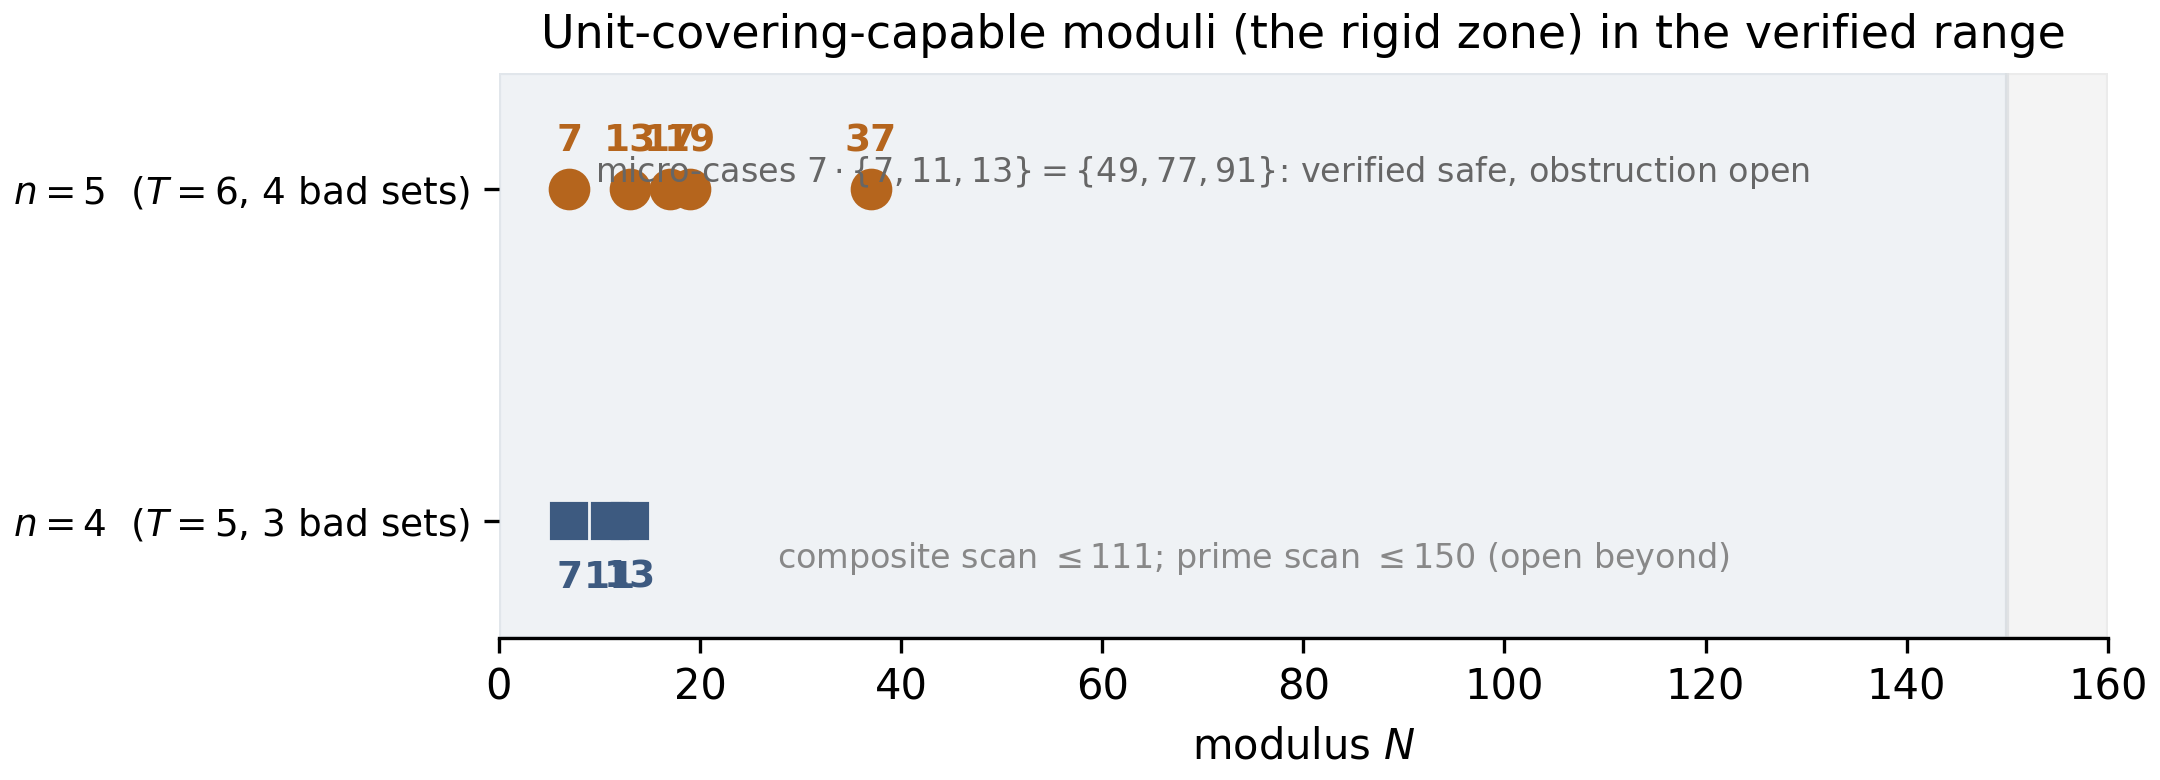
\includegraphics[max width=\textwidth, max height=0.32\textheight]
  {fig_rigidzone.png}
\end{center}

Three features of Table~\ref{tab:rigid} organize this section. First, the
zones are \emph{small and scattered}: no arithmetic progression, no
obvious multiplicative family---$17,19,37$ are not lifts of anything
smaller (they are prime, and prime moduli are their own base by
Lemma~\ref{lem:lift}). Second, the $n=4$ zone does not contain the $n=5$
zone and vice versa: $11$ is capable with three bad sets but not with
four---counting kills it, since four unit bad sets at $N=11$ ($h=1$,
$|B_w|=3$) have union of size at most $4\cdot 3-3=9<11$---while
$17,19,37$ are incapable with three bad sets and capable with four. The
rigid zone is a genuinely rung-dependent object. Third, within the
verified range the $n=5$ zone is \emph{constant} as the range grows:
after $37$, no modulus whatsoever (prime or composite) is capable, through
primes $150$ and composites $111$. We call this the rigid-zone map; it is
an empirical finding, stated with its range, and we emphasize that its
finiteness is not proved (Conjecture~\ref{conj:successor} is the natural
positive statement).

The rest of the section classifies the covering configurations at every
capable prime, at both rungs. The classifications are exact
if-and-only-if theorems; their proofs at $N\le 17$ are group-theoretic
(tilings and matchings), and at $19,37$ rest on an exhaustive finite check
whose verification record is in \S\ref{sec:sound}. Throughout,
$m=(N-1)/2$, $C=\Z_N^\ast/\{\pm1\}\cong\Z_m$, and by
Lemma~\ref{lem:class} a unit tuple covers $\Z_N$ iff the class sets
$X_w\cdot S_h$ cover $C$.

\subsection{The base rung: three bad sets}\label{sec:K4}

\begin{theorem}[$K_7$; $n=4$]\label{thm:K4}
Let $N=7$ ($h=1$, $C\cong\Z_3$). Three unit bad sets cover $\Z_7$ iff
their antipodal classes $\{\pm w_i^{-1}\}$ are the three distinct classes
of $\Z_7^\ast$. There are $4$ scale-normalized covering pairs
$(b,c)$ at $a=1$: $(2,3)$, $(2,4)$, $(3,5)$, $(4,5)$.
\end{theorem}

\begin{proof}
Here $S_h=S_1$ is a single class, so $B_w$ contributes exactly the class
$X_w$, and three bad sets cover iff $\{X_1,X_b,X_c\}=C$. The covering
pairs are read off $\Z_7^\ast$: the classes are
$\{1,6\},\{2,5\},\{3,4\}$; with $a=1$ contributing $\{1,6\}$, the pair
$(b,c)$ must contribute $\{2,5\}$ and $\{3,4\}$, i.e.\
$b\in\{2,5\}$, $c\in\{3,4\}$ with the classes of $b,c$ distinct and
completing $C$---enumerating gives exactly the four listed pairs.
\end{proof}

\begin{theorem}[$K_{11}$: domino adjacency]\label{thm:K11}
Let $N=11$ ($h=2$, $C\cong\Z_5$, generated by $g=\cls(2)$). Each unit
bad set covers the \emph{domino} $\{X_w,X_w g\}$ of $C$. Three dominos
$\{t_i,t_i+1\}$, $t_i\in\Z_5$, cover $C$ iff the complement of the start
set $T=\{t_1,t_2,t_3\}$ (two vertices of $C_5$) contains no adjacent
pair. There are $12$ scale-normalized covering pairs.
\end{theorem}

\begin{proof}
A vertex $p\in C$ is uncovered iff $p\notin T$ and $p-1\notin T$; since
$|T|=3$ and $|C|=5$, covering fails iff the two-element complement
contains an adjacent pair $\{p-1,p\}$. With the scale normalization
$w_1=1$ (so $e(X_1)=0\in T$) the admissible complements are
$\{1,3\},\{1,4\},\{2,4\}$---that is, the start sets
$\{0,2,4\},\{0,2,3\},\{0,1,3\}$---and each is realized by four
multisets $(1,b,c)$ (each of the two remaining starts is realized by two
residues, $b$ and $-b$, with the same class), giving $3\times 4=12$,
matching the direct scan.
\end{proof}

\begin{theorem}[$K_{13}$: coset tiling]\label{thm:K13}
Let $N=13$ ($h=2$, $C\cong\Z_6$, generated by $g=\cls(2)$). Three unit
bad sets cover $\Z_{13}$ iff their start classes $X_w$ form a coset
$\{X,\,Xg^2,\,Xg^4\}$ of the order-$3$ subgroup of $C$. There are $4$
scale-normalized covering pairs: $(3,4)$, $(3,9)$, $(4,10)$, $(9,10)$ at
$a=1$.
\end{theorem}

\begin{proof}
Each bad set covers the domino $\{X_w,X_wg\}$; three dominos on the
$6$-cycle cover iff they are pairwise disjoint (three sets of size two
covering six vertices). Disjointness of $\{t,t+1\}$ and $\{s,s+1\}$ on
$\Z_6$ is equivalent to $s-t\notin\{-1,0,1\}$, i.e.\ $s-t\in\{2,3,4\}$
up to sign. Three starts pairwise at such differences must be
$\{t,t+2,t+4\}$: if two starts differ by $3$, no third start is compatible
(differing from both by $\{2,3,4\}$ mod $6$), and the remaining
possibilities are exactly the cosets of $\{0,2,4\}$. The four listed
pairs are the realizations with $e(X_1)=0$ fixed.
\end{proof}

\subsection{The second rung: four bad sets}\label{sec:K5}

At $n=5$ the same three group-theoretic mechanisms persist at
$7$ and $13$ (now with four dominos: at $N=7$, four classes cover
$C_3$ iff they hit all three classes; at $N=13$, four dominos cover
$C_6$ iff the complement of the start set contains no adjacent pair), and
one new mechanism appears at $17$.

\begin{theorem}[$K_{17}$: perfect matching]\label{thm:K17}
Let $N=17$ ($h=2$, $C\cong\Z_8$; $c=\cls(2)$ has order $4$ since
$2^4\equiv-1 \pmod{17}$). Each unit bad set covers the domino
$\{X_w,X_wc\}$, and dominos live inside the two cosets of the order-$4$
subgroup $\langle c\rangle$, each coset a $4$-cycle under multiplication
by $c$. Four unit bad sets cover $\Z_{17}$ iff each coset contains
exactly two of the four starts and the two are non-adjacent in that
$4$-cycle (equivalently, differ by $c^2$). There are $16$
scale-normalized covering $4$-multisets.
\end{theorem}

\begin{proof}
Within one $4$-cycle $\{x,xc,xc^2,xc^3\}$, two dominos
$\{X,Xc\}$, $\{Y,Yc\}$ cover the cycle iff they are disjoint iff
$Y\notin\{X,Xc,Xc^{-1}\}$, i.e.\ $Y=Xc^2$. If one coset contained three
starts, the other would contain one, and a single domino covers only two
of its cycle's four vertices; if one coset contained all four, the other
would be untouched. Hence exactly two starts per coset, at antipodal
positions of the $4$-cycle. The count of scale-normalized realizations is
$16$, matching the direct scan; the sparsity is the matching constraint.
\end{proof}

\begin{example}[a covering at $17$, by hand]\label{ex:17}
The residues $(1,4,6,7)$ cover $\Z_{17}$:
\[
B_1\cup B_4\cup B_6\cup B_7
=\{0,\pm1,\pm2\}\cup\{0,\pm4,\pm9\}\cup\{0,\pm3,\pm6\}
 \cup\{0,\pm5,\pm10\}=\Z_{17},
\]
the eight classes $\{\pm1,\pm2,\pm4,\pm9,\pm3,\pm6,\pm5,\pm10\}$
exhausting $C_8$. This is realizable as a genuine speed set: the pair
$(1,16)$ of $V=(1,4,6,7,16)$ has effective residues $(1,4,6,7)$ on
$\Z_{17}$ and is a true (non-certifying) pair. Hand-checkable anchors of
this kind anchor every classification to the original problem.
\end{example}

At $N=19$ and $N=37$ the covering radius $h$ reaches $3$ and $6$, the
class segments $S_h$ grow past two elements, and the tiling gloss ends:
the classifications become explicit finite lists. Fix a generator
$g=\cls(2)$ of $C$ (at both moduli $2^{m}\equiv -1$, verified), write
$e(\cls(g)^t)=t$ for the \emph{exponent} of a class, and let
$S=e(S_h)\subseteq\Z_m$. By Lemma~\ref{lem:class}, a unit $4$-tuple
covers $\Z_N$ iff
\[
\bigcup_{i=1}^{4}\bigl(e(X_{w_i})+S\bigr)=\Z_m .
\]
Multiplying all four residues by a unit $u$ shifts every exponent by the
constant $-e(\cls u)$, so covering depends only on the \emph{translate
class} of the exponent multiset in $\Z_m$.

\begin{theorem}[$K_{19}$]\label{thm:K19}
Let $N=19$: $m=9$, $h=3$, $S=\{0,1,4\}$. Four unit bad sets cover
$\Z_{19}$ iff the exponent multiset $\{e(X_{w_i})\}$ is a translate of
\[
A=\{0,1,2,7\}\quad(\text{gaps }1,1,5,2)
\qquad\text{or}\qquad
B=\{0,2,4,6\}\quad(\text{gaps }2,2,2,3),
\]
the latter being the doubled interval $2\cdot\{0,1,2,3\}$. There are
exactly two covering translate classes and $64$ scale-normalized covering
residue $4$-multisets ($8$ residue realizations per class, all with four
distinct exponents).
\end{theorem}

\begin{theorem}[$K_{37}$]\label{thm:K37}
Let $N=37$: $m=18$, $h=6$, $S=\{0,1,2,5,8,9\}$. Four unit bad sets cover
$\Z_{37}$ iff the exponent multiset is a translate of the single class
\[
C_0=\{0,2,12,15\}\quad(\text{gaps }2,10,3,3).
\]
There is one covering translate class and $32$ scale-normalized covering
residue $4$-multisets.
\end{theorem}

\begin{proof}[Proof of Theorems~\ref{thm:K19} and \ref{thm:K37}]
The reduction to translate classes is proved above. The class lists are
then decided by exhaustive enumeration of all contains-$0$ $4$-multisets
of $\Z_m$ ($165$ candidates at $m=9$, $1{,}140$ at $m=18$---hand-checkable
scale), checking $\bigcup(e_i+S)=\Z_m$ exactly. Correctness of the
packaging was verified bidirectionally against the residue level: over
\emph{all} unit $4$-multisets ($5{,}985$ at $N=19$, $82{,}251$ at
$N=37$), the predicate ``exponent multiset is a translate of a listed
class'' agrees with direct bitmask covering, with zero mismatches in
either direction; the residue covering counts $64$ and $32$ were
reproduced by three independent implementations (bitmask, frozenset,
exponent-space). The full verification record is in \S\ref{sec:sound}.
\end{proof}

\begin{remark}[what the classifications say structurally]\label{rem:pattern}
Three structural facts deserve the reader's attention, because they are
the paper's central finding. First, \emph{every covering configuration at
every rigid prime has four distinct antipodal classes}: no covering
multiset repeats an exponent. This is consistent with
Lemma~\ref{lem:D3}: $19\equiv 1\pmod 6$ is exactly the case its $p_m=3$
bound cannot reach, and the classification shows covering there needs the
full $p_m=4$. Second, \emph{negation is not a symmetry} of the covering
problem: $B_{-w}=B_w$, so the negated tuple $(-w_i)$ is a genuinely
different tuple whose classes differ; the negation class of $B=\{0,2,4,6\}$
happens to be covering (it is negation-stable) while those of $A$ and
$C_0$ are not---negation acts as a diagnostic, never as an invariance,
and an earlier attempt to quotient by it was discarded as unsound. Third,
the character of the classification changes at $h\ge 3$: $K_{13}$ and
$K_{17}$ are group-theoretic statements (tilings, matchings) with slick
proofs, while $K_{19}$ and $K_{37}$ are finite lists. The classification
is complete but the tiling gloss does not persist---we read this as a
genuine change in the texture of the landscape, not as a gap in the
method.
\end{remark}

\subsection{Composite moduli}\label{sec:composites}

Composites split cleanly by parity (Proposition~\ref{prop:reach}): even
composites are never unit-capable, and odd composites are governed by the
reachability mechanism---a covering by unit bad sets must cover every
non-unit class, but unit bad sets reach non-unit classes only through
$j\le h$ with $\gcd(j,N)>1$. Table~\ref{tab:composites} records the
outcome for every odd composite in the open part of the range
($49$--$111$): a \emph{proved} safety whenever some non-unit class is
unreachable, and a handful of \emph{micro-cases} where all non-unit
classes are reachable, the slot counts do not obstruct, and no \emph{unit}
covering exists anyway (Table~\ref{tab:composites}; the qualification
``unit'' is load-bearing --- see Remark~\ref{rem:postcomposite}).

\begin{table}[htbp]
\centering
\small
\caption{Odd composites $49$--$111$ at $n=5$ ($T=6$): non-unit antipodal
classes, how many are reachable by unit bad sets (via
$j\le h$, $\gcd(j,N)>1$), and capability. All entries cross-checked by an
independent set-based scanner; zero capable moduli.}
\label{tab:composites}
\begin{tabular*}{\textwidth}{@{\extracolsep{\fill}} r r r r l}
\toprule
$N$ & $h$ & non-unit classes & reachable & status \\
\midrule
$49=7^2$      & 8  & 3  & \textbf{3} & micro-case (verified safe) \\
$51=3\cdot17$ & 8  & 9  & 8  & proved safe \\
$55=5\cdot11$ & 9  & 7  & 5  & proved safe \\
$57=3\cdot19$ & 9  & 10 & 9  & proved safe \\
$63$          & 10 & 13 & 12 & proved safe \\
$65=5\cdot13$ & 10 & 8  & 6  & proved safe \\
$69$          & 11 & 12 & 11 & proved safe \\
$75$          & 12 & 17 & 14 & proved safe \\
$77=7\cdot11$ & 12 & 8  & \textbf{8} & micro-case (verified safe) \\
$81=3^4$      & 13 & 13 & 12 & proved safe \\
$85=5\cdot17$ & 14 & 10 & 8  & proved safe \\
$87=3\cdot29$ & 14 & 15 & 14 & proved safe \\
$91=7\cdot13$ & 15 & 9  & \textbf{9} & micro-case (verified safe) \\
$93=3\cdot31$ & 15 & 16 & 15 & proved safe \\
$95=5\cdot19$ & 15 & 11 & 9  & proved safe \\
$99=9\cdot11$ & 16 & 19 & 18 & proved safe \\
$105=3\cdot5\cdot7$ & 17 & 28 & 25 & proved safe \\
$111=3\cdot37$ & 18 & 19 & 18 & proved safe \\
\bottomrule
\end{tabular*}
\end{table}

The micro-cases form a pattern too clean to be coincidence:
\[
49=7\cdot 7,\qquad 77=7\cdot 11,\qquad 91=7\cdot 13,
\]
that is, the products of $7$ with the $n=4$ rigid-zone primes
$\{7,11,13\}$. These are precisely the odd composites in range where
\emph{every} non-unit class is reachable, so the reachability mechanism is
silent, yet no unit covering exists; the obstruction is multiplicative.
The pattern predicts that the next
micro-cases, if any, should be sought at $7\cdot17=119$ and $7\cdot19=133$
(and $7\cdot37=259$), all outside the scanned composite range. We flag
this as an open problem (\S\ref{sec:open}) rather than a conjecture: three
data points do not make one.

\begin{remark}[post-submission development at the composite moduli]
\label{rem:postcomposite}
Work completed after this manuscript was assembled (companion note) changes
the micro-case picture in three ways, and the open problem is restated
accordingly in \S\ref{sec:open}. First, the \emph{fibration}: a bad set
whose speed has $d=\gcd(w,N)>1$ is the full preimage of a unit bad set at
$N/d$ with the \emph{same} threshold. Consequently kernel-speed coverings
\emph{do} exist at the micro-cases --- for example
$B_7\cup B_{14}\cup B_{21}=\Z_{49}$ is the transferred $K_7$ classification
--- so ``no covering at composites'' is false as a blanket statement; what
the micro-cases exclude is unit coverings, and more generally any covering
in which units are load-bearing. Second, the unit-side statement that
survives is \emph{no unit assistance}: at $N=p^2$ and $N=pq$ with
$p\ge5$, a covering family of at most four distinct bad sets with at most
two unit members has its kernel subfamily covering; three unit bad sets
never cover at all for $N\ge31$, $N\not\equiv0\pmod6$; and a pure-unit
family covers only above rigid-zone primes --- which makes the unit safety
of $77=7\cdot11$ a theorem rather than a verification (its reduction
demands a covering of $\Z_{11}$, and $11$ is not in the $n=5$ zone). Third,
the residual is explicit: the cells with three unit sets and at most one
kernel set, occupied at $N=9$ (a genuine unit-assisted covering, and the
reason the prime hypothesis cannot be dropped), verified empty at $p=5$
and throughout the tested composite range.

\medskip
Fourth (the $p^2$ closure, completing the companion note's programme):
the last open cell at square moduli --- one kernel set with three unit
sets --- is now \emph{empty at every prime $p\ge5$}.  For unit triples
whose residues are pairwise $\pm$-distinct mod $p$, the trichotomy
programme applies: Lemma~B ($p\equiv5\pmod6$) is proved for $p\ge17$
(the kills run on the contained census, Lemma T, clean from $p=17$, and
Corollaries T1--T3; a pre-T3 draft of the overlap kill had required
$p\ge23$), with $p=11$ closed by exhaustive finite case analysis (36
viable configurations, each carrying a positive residual-fit margin of at
least $2$, cross-validated by an independent brute force that reproduces
the known failure counts $50$ at $p=7$ and $2$ at $p=13$ exactly, the
$p=17$ finite analysis of the earlier draft now a redundant
verification); Lemma~A ($p\equiv1\pmod6$) is proved for $p\ge31$
unconditionally --- its one remaining input, the foot-count trichotomy
in its consumed form (the one-foot statement at the two size pairs
$(2k{+}2,2k{+}1)$ and $(2k{+}1,2k{+}1)$, viable differences confined to
$\{2,(p-1)/2\}$), is discharged by Lemma~\ref{lem:E} of
\S\ref{sec:lemmaE} (the three-distance foot count, proved for every
$p\ge31$ and cross-checked against the foot census of the previous
revision to $p\le419$) --- with $p=19$ closed the same way (614
viable configurations, margin $3$), and it is \emph{false} at $p=7,13$,
where $\pm$-distinct coverings exist and the cells are closed by direct
verification. For $\pm$-colliding units ---
two speeds equal up to sign mod $p$, a configuration the cell definition
does not exclude and the trichotomy lemmas do not reach --- a new argument
closes the case: the two colliding bad sets are shears of one another, so
their per-fiber $t$-space placements drift \emph{exactly linearly} in the
fiber index, while the fiber covering configurations are pinned (the
placements' difference set has at most $6$ elements, with covering counts
$28$ and $68$ per collision topology, \emph{independent of $p$}); a
pigeonhole over the $p-|B_k|$ kernel-uncovered fibers then kills every
family.  The mechanism is proved in general; its computational input is
stated as a named lemma with its verification range (every prime
$11\le p\le 113$), and the ground truth is an exhaustive enumeration of
$3.3$\,million colliding families at $p\le43$ with zero coverings, the
nearest families failing all but two fibers.

The closure's exact dependency structure is now recorded in
\S\ref{sec:groupring}, and it is sharper than ``modulo two computational
inputs'': of the two named inputs, one is now \emph{proved} --- the
foot-count inequality for the one-foot trichotomy (in the consumed form,
clean from $p\ge31$) is Lemma~\ref{lem:E} of \S\ref{sec:lemmaE}, an
elementary three-distance argument with no group-ring content --- so the
closure rests on a single unbounded hypothesis, the four-family covering
classification for the pinning lemma (verified to $p\le113$, and
subsuming the shear-rigidity input because the pinned per-fiber
configurations are exactly the classified families). The $pq$
side of \S\ref{sec:pq} now carries the same structure at semiprime moduli:
the $(1,1,2)$ and three-unit cells at $N=pq$ are verified empty to
$N\le143$ and reduce, by the row translation, to exactly the same
remaining input.
\end{remark}

\subsection{Discharging Input E: the three-distance foot count}\label{sec:lemmaE}

Input E in its consumed form (\S\ref{sec:gt-support}) is the one-foot
trichotomy at the two size pairs consumed by the kills M4 and M5 of
Lemma~A: at $p=6k+1$, an arithmetic progression $A(a,d,s)$ of critical
size $s\in\{2k{+}1,2k{+}2\}$ with at most one point outside
$I_1=[s_1,p-1]$ (where $(s_1,s)=(2k{+}2,2k{+}1)$ for M4 and
$(2k{+}1,2k{+}1)$ for M5) must have $\|d\|\in\{2,(p-1)/2\}$. This
subsection proves that statement outright for every prime $p\ge31$
(Lemma~\ref{lem:E} below) --- the discharge route identified in
\S\ref{sec:gt-support}, carried out by an elementary, self-contained
analysis of the rotation $j\mapsto jd\bmod p$: the three-distance
theorem of that rotation, in exactly the regime the consumers need. No
group-ring input is used. Throughout, $p=6k+1$ is prime, $3k=(p-1)/2$,
and $d$ is a $\pm$-representative in $[2,3k]$.

\paragraph{Notation.} For $s\ge2$ put
$X=X^{(s)}_d=\{jd\bmod p:0\le j<s\}$ (so $A(a,d,s)=a+X$), let
$x_1<\dots<x_s$ be its sorted elements and $g_i=x_{i+1}-x_i$ for $i<s$,
$g_s=p-x_s+x_1$ its cyclic gaps; the pair sums $g_i+g_{i+1}$ (indices
mod $s$) are the spans $\mathrm{next}(x)-\mathrm{prev}(x)$ over $x\in
X$, and $G_2(X)=\max_i(g_i+g_{i+1})$. Recall
$\mathrm{feet}(A)=s-|A\cap I_1|$, the number of points of $A$ in
$[0,s_1)$. For $R\subseteq\Z_n$ with $0\in R$, sorted
$0=\rho_1<\dots<\rho_t$, let $\Gamma_2(R;n)$ be the largest sum of
cyclically adjacent gaps of $R$ on $\Z_n$ (the last gap being
$n-\rho_t$; $t=1$: $\Gamma_2=2n$), and write
$\gamma^{\mathrm f}(R)=\rho_2$ (first gap) and
$\gamma^{\mathrm w}(R;n)=n-\rho_t$ (wrap gap).

\begin{lemma}[feet and pair sums]\label{lem:E0}
For $X\subseteq\Z_p$ with $|X|\ge2$ and $2\le L\le p$: every cyclic
interval of $L$ consecutive residues meets $X$ in at least two points
iff $G_2(X)\le L$. In particular,
$\min_a\mathrm{feet}(A(a,d,s))\ge2$ iff $G_2(X^{(s)}_d)\le s_1$.
\end{lemma}

\begin{proof}
An $L$-interval $[u,u+L)$ contains at most one point of $X$ iff some
$x\in X$ has $\mathrm{prev}(x)<u$ and $u+L\le\mathrm{next}(x)$: for the
unique point of a one-point instance this is immediate, and for an empty
instance it holds with $x$ the first point at or after $u+L$. Either
way $\mathrm{span}(x)\ge L+1$; conversely a point of span $\ge L+1$
produces the one-point interval $[\mathrm{prev}(x)+1,\,
\mathrm{prev}(x)+L+1)$. For the second claim,
$\#(a+X)\cap[0,s_1)=\#X\cap([0,s_1)-a)$, and $([0,s_1)-a)$ runs through
all cyclic $s_1$-intervals as $a$ does.
\end{proof}

\begin{lemma}[column decomposition]\label{lem:E1}
Let $s\in\{2k{+}1,2k{+}2\}$, $2\le d\le3k$, and
$W=\floor{d(s-1)/p}\ge1$; write $r=p\bmod d$, $\sigma=d-r$,
$m_0=\floor{p/d}$, and $c_w=(-wp)\bmod d\in[0,d)$ for $0\le w\le W$.
Then: \textup{(i)} $c_0,\dots,c_W$ are distinct; \textup{(ii)} the $j$
with $\floor{dj/p}=w$ form the interval
$[\lceil wp/d\rceil,\,\min(\lceil(w{+}1)p/d\rceil-1,\,s-1)]$, and the
corresponding points $jd\bmod p=dj-wp$ are exactly
$c_w,c_w+d,\dots,c_w+(h_w-1)d$, where
$h_w=\lceil(w{+}1)p/d\rceil-\lceil wp/d\rceil$ for $w<W$ and
$h_W=s-\lceil Wp/d\rceil$; \textup{(iii)} for $w<W$ the run is the
\emph{full} column $\{x\in[0,p):x\equiv c_w\pmod d\}$ --- of height
$F(c)=m_0+1$ for $c<r$ and $m_0$ otherwise, with top $p-d+c_{w+1}$ ---
while run $W$ is the prefix of the column of $c_W$ of height
$h_W\le F(c_W)$, with top $H=d(s-1)-Wp$.
\end{lemma}

\begin{proof}
(i) $p$ is prime and $d<p$, so $\gcd(p,d)=1$; and
$W\le d(s-1)/p\le d(2k+2)/(6k+1)<d$, so $w\mapsto wp\bmod d$ is
injective on $[0,W]$. (ii) $\floor{dj/p}=w$ iff $wp\le dj<(w+1)p$, i.e.\
$j\in[\lceil wp/d\rceil,\lceil(w+1)p/d\rceil-1]$, truncated at $s-1$;
the sequence $\floor{dj/p}$ increases in steps of $0$ or $1$ (as $d<p$),
so every $w\le W$ occurs. The first point of run $w$ is
$d\lceil wp/d\rceil-wp\in[0,d)$ with residue $\equiv-wp\equiv c_w$, so
it equals $c_w$; the run then steps by $d$ within its column. (iii) For
$w<W$ the last point is
$d(\lceil(w{+}1)p/d\rceil-1)-wp=p-d+\beta_w$, where
$\beta_w=d\lceil(w{+}1)p/d\rceil-(w{+}1)p\in[0,d)$ is the canonical
representative of $c_{w+1}$. This top lies in $[p-d,p)$ and satisfies
$p-d+\beta_w\equiv r+c_{w+1}\equiv c_w\pmod d$ (since
$c_{w+1}\equiv c_w+\sigma$ and $r+\sigma=d$); being congruent to $c_w$
and in $[p-d,p)$ it is the top of the full column of $c_w$, whose
$F(c)=\lceil(p-c)/d\rceil$ elements are $c,c+d,\dots$ --- so run $w$ is
that full column and $h_w=F(c_w)$. Run $W$ spans
$j\in[\lceil Wp/d\rceil,s-1]$, hence is the bottom prefix of height
$h_W=s-\lceil Wp/d\rceil\le F(c_W)$, with top $d(s-1)-Wp$.
\end{proof}

\begin{lemma}[bands and the pair-sum identity]\label{lem:E2}
In the setting of Lemma~\ref{lem:E1} with $W\ge1$, put
$C=\{c_0,\dots,c_W\}$, $C^-=C\setminus\{c_W\}$, $h=h_W$, and
$T=(C^-\cap[0,r))\cup E$ with $E=\{c_W\}$ if $h>m_0$ and $E=\emptyset$
otherwise. Then:
\textup{(i)} for $0\le i\le m_0$, the residues of $X$ in the band
$[id,(i{+}1)d)$ are exactly $R_i=C$ if $i<h$, $R_i=C^-$ if
$h\le i\le m_0-1$, and $R_{m_0}=T$; in particular
$R_0\supseteq\dots\supseteq R_{m_0}$, all containing $0$;
\textup{(ii)} the gap sequence $(g_1,\dots,g_s)$ is the concatenation,
over $i=0,\dots,m_0-1$, of the cyclic gap block of $R_i$ on $\Z_d$
(consecutive differences of $R_i$, ending with the wrap gap
$d-\max R_i$), followed by the top block of $T$ (consecutive
differences, ending with $r-\max T$);
\textup{(iii)} the pair sums of $X$ are the cyclic two-step gaps of
these blocks --- a singleton band contributing the double wrap $2d$,
attained iff the band below is also a singleton; singleton bands occur
only for $W=1$ --- together with the boundary pairs
$\gamma^{\mathrm w}(R_{i-1};d)+\gamma^{\mathrm f}(R_i)$ (reading
$\gamma^{\mathrm f}=d$ for a singleton band), of which those with
$i\le m_0-1$ are at most $\gamma^{\mathrm w}(R_i;d)+\gamma^{\mathrm
f}(R_i)\le\Gamma_2(R_i;d)$ by (i), together with the two outer pairs
\[
\mathrm{span}_0=(r-\max T)+\gamma^{\mathrm f}(C),\qquad
\mathrm{span}^\ast=(d-\max R_{m_0-1})+\begin{cases}
\gamma^{\mathrm f}(T)&|T|\ge2,\\ r&|T|=1.\end{cases}
\]
Consequently, for $W\ge2$,
\[
G_2(X)=\max\bigl(\Gamma_2(C;d),\ \Gamma_2(C^-;d)\ \text{[if $h\le
m_0-1$]},\ \Gamma_2(T;r)\ \text{[if $|T|\ge2$]},\
\mathrm{span}_0,\ \mathrm{span}^\ast\bigr),
\]
while for $W=1$, $G_2(X)\le2d$.
\end{lemma}

\begin{proof}
(i) By Lemma~\ref{lem:E1}, $X$ is the union of the runs, run $w$
occupying bands $0,\dots,h_w-1$ at residue $c_w$. For $i\le m_0-1$ every
full run is present ($h_w=F(c_w)\ge m_0>i$), and run $W$ is present iff
$h>i$; hence $R_i=C$ for $i<h$ and $C^-$ otherwise. Band $m_0$ sees
exactly the full runs with $F(c_w)>m_0$, i.e.\ $c_w<r$, plus run $W$ iff
$h>m_0$: that is $T$. The nesting is immediate, and $0=c_0\in C^-$ (as
$W\ge1$) with $0<r$ puts $0$ in every band. (ii) Band $i$'s points, in
increasing order, are $c+id$ with $c\in R_i$ in residue order, so the
within-band gaps are the residue differences; the gap from band $i$'s
last point to band $i{+}1$'s first (residue $0$, since $0\in
R_{i+1}$) is $d-\max R_i$; and the final wrap, from $\max T+m_0d$ to
$0$, is $r-\max T$ (as $p=m_0d+r$). (iii) The pair sum around a point
of band $i$ is either within-block (a two-step gap of $R_i$; around the
band's last point it is the last two gaps of the block, equally a
two-step gap) or crosses the boundary below, where it is the last gap
of block $i-1$ plus the first gap of block $i$; for $i\le m_0-1$ the
nesting (i) gives $\gamma^{\mathrm w}(R_{i-1};d)\le\gamma^{\mathrm
w}(R_i;d)$, and the wrap and first gaps are cyclically adjacent, so the
boundary pair is at most $\Gamma_2(R_i;d)$. A singleton band $R_i=\{0\}$
arises only when $C^-=\{0\}$, i.e.\ $W=1$; its lone point has pair sum
$\gamma^{\mathrm w}(R_{i-1};d)+d$, which equals $2d$ exactly when
$R_{i-1}=\{0\}$ as well. The top band contributes the two-step gaps of
$T$ on $[0,r)$ (only for $|T|\ge2$; around $T$'s last point the pair is
the last within-gap plus $r-\max T$, again a two-step gap on $\Z_r$),
the boundary pair $\mathrm{span}^\ast$ around $m_0d$, and --- around
$0$ --- the outer pair $\mathrm{span}_0$. For $W\ge2$ no band is a
singleton ($|C^-|=W\ge2$), so every pair sum is at most the maximum of
the five displayed quantities; conversely each of the five is realized
as a pair sum of $X$ ($\Gamma_2(C)$ in band $0$; $\Gamma_2(C^-)$ in a
$C^-$-band, which exists exactly when $h\le m_0-1$; $\Gamma_2(T;r)$ in
the top band; $\mathrm{span}_0$ around $0$; $\mathrm{span}^\ast$ around
$m_0d$). For $W=1$: $\Gamma_2(C;d)=d$, the singleton-band terms are at
most $2d$, $\mathrm{span}_0\le d$, and $\mathrm{span}^\ast<2d$: if $|T|=1$
then $R_{m_0-1}\in\{C,C^-\}$ gives $(d-\sigma)+r=2r$ resp.\ $d+r$,
both $<2d$; if $|T|=2$ then $h=m_0+1$, $R_{m_0-1}=C$, and
$(d-\sigma)+\gamma^{\mathrm f}(T)<(d-\sigma)+r=d$. Hence $G_2\le2d$.
\end{proof}

\begin{lemma}[wrap count]\label{lem:E3}
For $k\ge2$ and $s=2k{+}1$: $W\ge d-2k+1$ for $3\le d\le3k-2$, $W=d-2k$
at $d=3k-1$, and $W=d-2k-1$ at $d=3k$. For $s=2k{+}2$: $W\ge d-2k+1$
for $3\le d\le3k-2$, and $W=d-2k$ at $d\in\{3k-1,3k\}$.
\end{lemma}

\begin{proof}
Since $d-2k+1$ is an integer, $W=\floor{d(s-1)/p}\ge d-2k+1$ iff
$d(s-1)\ge(d-2k+1)p$, a quadratic inequality in $d$. For $s=2k+1$ it
reads $d(4k+1)\le12k^2-4k-1$, i.e.\
$d\le3k-1-\frac{3k}{4k+1}<3k-1$, so it holds for $d\le3k-2$ --- for
$d\le2k$ trivially, since then $d-2k+1\le1\le W$ (with $W=0\ge4-2k$ at
$d=3$, and $W\ge1$ for $d\ge4$). The endpoint values are direct:
$W=\floor{2k(3k-1)/(6k+1)}=k-1=d-2k$ and $W=\floor{6k^2/(6k+1)}=k-1$.
For $s=2k+2$ the inequality reads $4kd\le12k^2-4k-1$, i.e.\
$d\le3k-1-\frac1{4k}$, again $d\le3k-2$ (for $d\le2k$ trivially:
$d-2k+1\le1\le W$, $W\ge1$ for $d\ge3$), with endpoints
$W=\floor{(2k+1)(3k-1)/(6k+1)}=k-1$ and
$W=\floor{3k(2k+1)/(6k+1)}=k$.
\end{proof}

\begin{lemma}[auxiliary bounds]\label{lem:E4}
In the setting of Lemmas~\ref{lem:E1}--\ref{lem:E2}:
\textup{(a)} for $R\subseteq\Z_n$ with $0\in R$ and $2\le|R|\le n$,
$\Gamma_2(R;n)\le n-|R|+2$;
\textup{(b)} if $d\le3k-1$ then $r\le2k-1$;
\textup{(c)} $\max C\le\max T+\sigma$;
\textup{(d)} $\mathrm{span}_0\le\Gamma_2(C;d)$;
\textup{(e)} if $W\ge2$ then $\mathrm{span}^\ast\le d-W+2$.
\end{lemma}

\begin{proof}
(a) Let $t=|R|$ and let the cyclic gaps be $\gamma_1,\dots,\gamma_t$
(summing to $n$, each $\ge1$). Every two-step gap is
$\gamma_i+\gamma_{i\pm1}\le\gamma_{\max}+\gamma'$, where $\gamma'$ is
the largest of the other $t-1$ gaps and hence at most
$(n-\gamma_{\max})/(t-1)$; the map $\gamma\mapsto\gamma+(n-\gamma)/(t-1)$
is increasing (constant when $t=2$), and
$\gamma_{\max}\le n-t+1$ by the pigeonhole principle, so
$\Gamma_2\le(n-t+1)+1=n-t+2$.
(b) If $d\le2k$ then $r\le d-1$; if $2k+1\le d\le3k-1$ then
$2d\le6k-2<p$ and $3d\ge6k+3>p$, so $m_0=2$ and
$r=p-2d\le6k+1-4k-2=2k-1$.
(c) The orbit moves by $c_{w+1}=c_w+\sigma$ when $c_w<r$ (no wrap:
$c_w+\sigma<r+\sigma=d$) and by $c_{w+1}=c_w-r$ when $c_w\ge r$; hence
any orbit point $x\ge\sigma$ is $c_w+\sigma$ with $c_w=x-\sigma\in[0,r)$.
If moreover $x\ne c_W$ then $c_w\in C^-\cap[0,r)\subseteq T$, so
$x\le\max T+\sigma$; for $x=c_W\ge\sigma$ the same argument uses
$c_{W-1}=c_W-\sigma\in C^-\cap[0,r)\subseteq T$ ($W\ge1$, so $c_{W-1}$
exists). An orbit point $x$ with $r\le x<\sigma$ (possible only when
$\sigma>r$) satisfies $x<\sigma\le\max T+\sigma$; a point of
$C^-\cap[0,r)$ is at most $\max T$; and $c_W<\sigma$, $x=0$ are
immediate. So every $x\in C$ has $x\le\max T+\sigma$.
(d) By (c), $r-\max T=(d-\sigma)-\max T\le d-\max
C=\gamma^{\mathrm w}(C;d)$; the wrap and first gaps are cyclically
adjacent, so $\mathrm{span}_0\le\gamma^{\mathrm w}(C;d)+\gamma^{\mathrm
f}(C)\le\Gamma_2(C;d)$.
(e) Reflect the orbit: $C\setminus\{0\}=\{d-m:m\in M\}$ with
$M=\{wr\bmod d:1\le w\le W\}$, and $C^-\setminus\{0\}=\{d-m:m\in M^-\}$
with $M^-=\{wr\bmod d:1\le w\le W-1\}$; thus $d-\max C=\min M=:\mu\le
\min M^-=:\mu^-$, so $d-\max R_{m_0-1}$ is $\mu$ or $\mu^-$, and the
elements of $T\setminus\{0\}$ are reflections $d-m$ of multiples
$m\in(d-r,\,d)$. If $|T|=1$: no multiple of $M^-$ lies in $(d-r,d)$
(its reflection would lie in $C^-\cap(0,r)\subseteq T\setminus\{0\}$),
so the $W-1$ distinct integers of $M^-$ lie in $[1,d-r]$ and
$\mu^-\le(d-r)-(W-2)=d-W+2-\sigma$, whence
$\mathrm{span}^\ast\le\mu^-+r\le d-W+2$. If $|T|\ge2$, let
$t=\gamma^{\mathrm f}(T)=\min(T\setminus\{0\})$. When $t\in C^-$: no
multiple of $M^-$ lies above $m_t=d-t$ (its reflection would lie in
$C^-\cap(0,t)$, below $t$), so $M^-\subseteq[\mu^-,m_t]$ gives
$m_t\ge\mu^-+W-2$ and
$\mathrm{span}^\ast\le\mu^-+(d-m_t)\le d-W+2$. When $t=c_W$ (which
forces $h>m_0$ and $c_W<r$, i.e.\ $m_W=d-c_W\in(d-r,d)$, and
$R_{m_0-1}=C$): no multiple at all lies above $m_W$ (a smaller-index
one would reflect into $C^-\cap(0,c_W)$ below $t$, and index $W$ is
$m_W$ itself), so $M\subseteq[\mu,m_W]$ gives $m_W\ge\mu+W-1$ and
$\mathrm{span}^\ast=\mu+(d-m_W)\le d-W+1$.
\end{proof}

\begin{lemma}[three-distance foot count; Input E discharged]\label{lem:E}
Let $p=6k+1$ be prime with $k\ge5$, let $d\in[3,3k-1]$, and let
$s\in\{2k{+}1,2k{+}2\}$. Then $G_2(X^{(s)}_d)\le2k+1$. Consequently, at
both consumer pairs $(s_1,s)=(2k{+}2,2k{+}1)$ and $(2k{+}1,2k{+}1)$,
$\min_a\mathrm{feet}(A(a,d,s))\ge2$ for every $d\in[3,3k-1]$: the
one-foot viable set is contained in $\{2,(p-1)/2\}$, which is Input E
in its consumed form, and Lemma~A is proved for $p\ge31$.
\end{lemma}

\begin{proof}
\emph{Case $W=0$.} Only $d=3$, $s=2k{+}1$: $X=\{0,3,\dots,6k\}$ has
gaps $3,\dots,3,1$, pair sums $6$ and $4$; $G_2=6\le2k+1$.
\emph{Case $W=1$.} Then $p\le d(s-1)<2p$, which at $s=2k{+}1$ gives
$d\in\{4,5,6\}$ and at $s=2k{+}2$ gives $d\in\{3,4,5\}$; by
Lemma~\ref{lem:E2}(iii), $G_2\le2d$. If $d\le5$ then
$G_2\le10\le2k+1$ (as $k\ge5$). If $d=6$ (so $s=2k{+}1$): here $r=1$,
$m_0=k$, and $h=s-F(0)=k$, so no band is a singleton, $T=\{0\}$,
$\mathrm{span}^\ast=2r=2$, and $G_2\le\max(d,\mathrm{span}_0\le d,
\mathrm{span}^\ast)=6\le2k+1$.
\emph{Case $W\ge2$, $d\le3k-2$.} Lemma~\ref{lem:E3} gives
$W\ge d-2k+1$, and no band is a singleton (that would force
$C^-=\{0\}$, i.e.\ $W=1$). Lemma~\ref{lem:E2}(iii) and
Lemma~\ref{lem:E4} bound each candidate:
$\Gamma_2(C;d)\le d-W+1\le2k$ (Lemma~\ref{lem:E4}(a) with $|C|=W+1$);
$\Gamma_2(C^-;d)\le d-W+2\le2k+1$ (same, $|C^-|=W\ge2$; only if it
occurs); $\Gamma_2(T;r)\le r-|T|+2\le r\le2k-1$
(Lemma~\ref{lem:E4}(a),(b); only if $|T|\ge2$);
$\mathrm{span}_0\le\Gamma_2(C;d)\le2k$ (Lemma~\ref{lem:E4}(d));
$\mathrm{span}^\ast\le d-W+2\le2k+1$ (Lemma~\ref{lem:E4}(e)). Hence
$G_2\le2k+1$.
\emph{Case $d=3k-1$.} Here $r=3$, $\sigma=3k-4$, $W=k-1$
(Lemma~\ref{lem:E3}), and, since $p\equiv3\pmod d$,
$c_w=(-3w)\bmod d$; as $3w\le3k-3<d$ for $w\le k-1$,
$C=\{0\}\cup\{d-3w:1\le w\le k-1\}=\{0,2,5,\dots,3k-4\}$, an
arithmetic progression with difference $3$ together with $0$, with
cyclic gaps $2,3,\dots,3$ and $\Gamma_2(C;d)=6$. Full columns have
$F(0)=3$ and $F(c)=2$ for $c\ge3$, so
$\sum_{c\in C^-}F(c)=3+2(k-2)=2k-1$ and $h=s-(2k-1)\in\{2,3\}$: in
either case $h\ge m_0=2$, so $C^-$ never occurs as a band set;
$T=\{0\}$ (at $s=2k{+}1$) resp.\ $T=\{0,2\}$ (at $s=2k{+}2$);
$\Gamma_2(T;3)\le3$; $\mathrm{span}_0\le3+2=5$;
$\mathrm{span}^\ast=(d-\max C)+r=3+3=6$. So $G_2=6\le2k+1$.
Finally, the primes $6k+1$ with $k\le4$ are $7,13,19$ ($25$ is not
prime); at $p=7$ the range $[3,3k-1]$ is empty, and $13,19$ are
Lemma~A's finite-cased primes, so $k\ge5$ is exactly $p\ge31$. The
consequence on viable sets follows from Lemma~\ref{lem:E0} together
with the endpoint values recorded in Remark~\ref{rem:Esharp}.
\end{proof}

\begin{remark}[endpoints and sharpness]\label{rem:Esharp}
The two excluded differences carry exact values. First,
$G_2(X^{(2k+1)}_2)=2k{+}3$: the progression $\{0,2,\dots,4k\}$ has gaps
$2,\dots,2,2k{+}1$, and the two outer pair sums are $2k+3$. Second,
$G_2(X^{(s)}_{3k})=2k{+}2$ for both $s$: at $s=2k{+}1$ through
$\Gamma_2(C;d)$ with $C=\{0\}\cup\{2k{+}1,\dots,3k-1\}$; at
$s=2k{+}2$ through $\Gamma_2(C^-;d)$ with
$C^-=\{0\}\cup\{2k{+}1,\dots,3k-1\}$, which occurs since then $h=1$
--- in both cases the dead residue run $[1,2k]$ plus one cluster gap.
Meanwhile $G_2(X^{(2k+1)}_{3k-1})=6$ (the case $d=3k-1$ above). These
are exactly the one-foot exceptions $\{2,(p{-}1)/2\}$ of the consumed
form. The clean threshold is sharp: at $d=5$ every $p\ge31$ has
$G_2=2d=10$ (the two-column case with two consecutive singleton bands:
$m_0-h=2\floor{(6k+1)/5}-2k\ge2$ for $k\ge4$), and $10\le2k+1$ first
holds at $k=5$, i.e.\ $p=31$; at $p=19$ the dirty differences are
$d\in\{4,5\}$, each with $G_2=8$ ($2d=8$ resp.\
$\mathrm{span}^\ast=2r=8$), at $p=13$ they are $d\in\{3,4,5\}$ with
$G_2\in\{6,8,10\}$ --- matching the census of \S\ref{sec:gt-support}
exactly. For large $p$ the maximum of $G_2$ over $d\in[3,3k-1]$ grows
like $\tfrac23(2k+1)$ (attained near $d=2k$, where $r=1$ and the orbit
is the cluster $\{0\}\cup\{d-W,\dots,d-1\}$), so the bound is generous
asymptotically; its binding cases are the two-column ones at small
$d$.
\end{remark}

\paragraph{Machine verification.}
The full architecture of this subsection is machine-checked by
\texttt{lemmaE\_\allowbreak master.py} (output
\texttt{out\_\allowbreak lemmaE.json}): the
column decomposition, the band identity, the block identity for the gap
sequence, and the pair-sum identity of Lemma~\ref{lem:E2} --- as an
exact equality, not merely a bound --- hold at every $(p,d,s)$ with
$p\le500$ ($45$ primes, $10{,}410$ triples); the bounds of
Lemma~\ref{lem:E4} are checked on every occurring set;
Lemma~\ref{lem:E} is verified directly to $p\le2000$ ($136{,}806$
evaluations) and, through the verified identity, to $p\le4000$
($367{,}986$ further checks, cross-checked against direct evaluation
along the way); the endpoint and dirty-prime values of
Remark~\ref{rem:Esharp} are exact; and Lemma~\ref{lem:E0}'s equivalence
reproduces all $76$ consumed-pair viable sets of the foot census
(\S\ref{sec:gt-support}) verbatim at every prime $p\le419$. Two
structural facts were confirmed exactly and are recorded for future
use: the class orbit $C$ is a rotation segment (the three-distance
structure), and its low part $C\cap[0,r)$ is itself a rotation segment
on $\Z_r$ with step $\sigma\bmod r$ --- the Euclidean recursion
$d\mapsto r$, which explains the uniformity of the analysis in $d$ but
which the proof above does not need.

With Lemma~\ref{lem:E}, Input E is discharged: the kills M4 and M5 of
Lemma~A receive their one-foot input unconditionally at every prime
$p\ge31$, and the $p^2$ and $pq$ closures of \S\ref{sec:composites} and
\S\ref{sec:pq} now rest on a single unbounded input, Input S. Their
dependency statements are updated accordingly.

\subsection{The non-porting, and the successor conjecture}

At $n=4$ the program's earlier work isolated a clean statement: no
invertible \emph{triple} of bad sets covers $\Z_N$ for any prime
$N\ge 17$ (verified for all unit triples at every modulus $N\le 60$, with
hand proofs at $17$ and $19$). This \emph{no-covering conjecture} does
\emph{not} port to $n=5$: $17$, $19$, and $37$ are capable with four bad
sets (Example~\ref{ex:17}). What generalizes is not the conjecture but the
framework---the covering language, the class reduction, and the
classification program---which at $n=5$ produced a different zone and a
complete list of its covering configurations. The failure mode is
instructive: the obstruction at $n=4$ was never ``three sets cannot
cover'' as a counting matter (three unit bad sets at a large prime have
union at most $3(2h+1)-2\approx \tfrac35 N$), it was the multiplicative
tiling constraint; adding a fourth set releases exactly the primes whose
class segments $S_h$ are large enough to tile with four translates.

The natural successor statement at $n=5$ is:

\begin{conjecture}[successor no-covering]\label{conj:successor}
For every prime $N\ge 41$, four unit bad sets never cover $\Z_N$
(equivalently: the $n=5$ rigid zone is exactly $\{7,13,17,19,37\}$).
\end{conjecture}

\noindent Verified within the scan range ($N\le 150$, prime; composites
$\le 111$; capability cross-checked by an independent set-based
implementation at every danger modulus). Note that counting never
obstructs here: for $N\ge 41$ one has $4(2h+1)-3\ge N$, so the
conjecture, if true, is a genuinely multiplicative statement about four
translates of $S_h$ in $\Z_{(N-1)/2}$---the same genre of statement as
the $n=4$ conjecture, one rung up. We do not attack it in this paper; the
verified range is stated, the conjecture is open, and the finiteness of
the rigid zone in general is open.

% ======================================================================
% Section 5 — The group-ring translation
% ======================================================================

\section{The group-ring translation}\label{sec:groupring}

The covering lemmas of the $p^2$ programme (Lemmas A and B of the companion
notes) are statements about three arithmetic progressions covering $\Z_p$.
This section re-encodes them \emph{exactly} as a statement about one sparse
identity in the group ring $\Z[\Z_p]\cong\Z[z]/(z^p-1)$: the obstruction
becomes the coefficient-sign pattern of a quotient of a $24$-term element by
an $8$-term element. The translation is proved (Theorem~\ref{thm:GT}), not
merely verified, and it is unconditional --- the identity holds for
\emph{every} configuration, and covering is exactly a positivity condition on
its solution. The machine verification then establishes, over an independent
code path, a census law: at every prime tested, the critical coverings fall
into exactly four difference families with placement counts \emph{independent
of $p$} (\S\ref{sec:gt-census}). This is the same pinning phenomenon that the
shear-rigidity argument measured fiberwise, now visible as a statement about
the identity itself, and it converts the programme's computational inputs
from vague debt into precisely stated, named lemmas with identified
discharge paths (\S\ref{sec:gt-support}) --- one of which, the foot-count
lemma, is now proved (Lemma~\ref{lem:E}, \S\ref{sec:lemmaE}).

The motive is the classical line connecting covering systems to roots of
unity: the Mirsky--Newman--Davenport--Rado theorem --- in an exact covering
system of $\Z$ the largest modulus repeats --- is proved by evaluating a
generating function at roots of unity and reading off pole structure
\cite{MirskyNewman}. Lemmas A and B are the cyclic, three-term analogue, and
the group ring is where that analogy becomes literal.

\subsection{The identity and the translation theorem}\label{sec:gt-identity}

Fix a prime $p$ and a \emph{configuration}: three arithmetic progressions
$A_i=\{a_i+jd_i \bmod p:0\le j<s_i\}$ in $\Z_p$ with $d_i\in\Z_p^{*}$,
$s_i\ge 1$. Write $\mathbf 1_i$ for the indicator of $A_i$ and define the
\emph{signed excess}
\[
\varepsilon(x)\;:=\;\sum_{i=1}^{3}\mathbf 1_i(x)-1\;\in\;\{-1,0,1,2\},
\qquad
E(z)\;:=\;\sum_{x\in\Z_p}\varepsilon(x)\,z^x .
\]
Work in the group ring $R_p:=\Z[z]/(z^p-1)$, and put
\begin{align*}
Q(z)\;&:=\;\sum_{i=1}^{3} z^{a_i}\,\bigl(1-z^{d_i s_i}\bigr)
        \prod_{j\ne i}\bigl(1-z^{d_j}\bigr),\\[\medskipamount]
P(z)\;&:=\;\prod_{i=1}^{3}\bigl(1-z^{d_i}\bigr).
\end{align*}
Both are sparse: $Q$ has at most $8\times 3=24$ terms with coefficients
$\pm1$ (each summand is the inclusion--exclusion of the box
$a_i+\{0,d_is_i\}+\{0,d_j\}+\{0,d_k\}$), and $P$ has at most $8$ terms. Let
$\overline\Phi_p:=\sum_{x\in\Z_p}z^x$ denote the all-ones element of $R_p$
(the reduction of the cyclotomic polynomial $\Phi_p$).

\begin{theorem}[group-ring translation]\label{thm:GT}
\;\textup{(i)} For \emph{every} configuration,
\[
Q \;=\; E\cdot P \qquad\text{in } R_p .
\]
\textup{(ii)} The configuration covers $\Z_p$ if and only if
$\varepsilon\ge 0$ pointwise. Consequently, writing
$\mathrm{ov}:=\sum_i s_i-p$, if $\mathrm{ov}=0$ then covering is equivalent
to $E=0$; if $\mathrm{ov}=1$ to $E=z^e$ for some $e$; and if
$\mathrm{ov}=2$ to $E\in\{z^e+z^f,\;2z^e\}$.
\textup{(iii)} The kernel of multiplication by $P$ on $R_p$ is exactly
$\Z\cdot\overline\Phi_p$, and $E$ is the \emph{unique} $X\in R_p$ with
$Q=XP$ and $X(1)=\mathrm{ov}$.
\end{theorem}

\begin{proof}
(i) Let $\omega=e^{2\pi i/p}$ and evaluate at $z=\omega^\ell$,
$\ell\in\Z_p$. For $\ell\ne 0$, since $d_i\in\Z_p^{*}$,
\[
\widehat{\mathbf 1}_{A_i}(\ell)
=\sum_{j<s_i}\omega^{\ell(a_i+jd_i)}
=\omega^{\ell a_i}\,\frac{1-\omega^{\ell d_i s_i}}{1-\omega^{\ell d_i}},
\]
a geometric sum with nonzero denominator. Summing the function identity
$\sum_i\mathbf 1_i=1+\varepsilon$ over $x\in\Z_p$ against $\omega^{\ell x}$
kills the constant $1$ at $\ell\ne0$, giving
$\sum_i\widehat{\mathbf 1}_i(\ell)=\widehat\varepsilon(\ell)$; multiplying by
$P(\omega^\ell)=\prod_j(1-\omega^{\ell d_j})\ne 0$ yields
$Q(\omega^\ell)=\widehat\varepsilon(\ell)P(\omega^\ell)$, i.e.\ the
polynomial $Q-E\cdot P$ vanishes at every nontrivial $p$-th root of unity.
At $\ell=0$ both sides vanish: $Q(1)=0$ because each summand contains the
factor $1-z^{d_is_i}$ at $z=1$, and $E(1)P(1)=\mathrm{ov}\cdot 0=0$. So
$Q-E\cdot P$ vanishes at all $p$ roots of $z^p-1$; a polynomial with integer
coefficients divisible by $z^p-1$ over $\mathbb{Q}$ (the roots are distinct) is
divisible over $\Z$ (monic divisor, Gauss's lemma), and exponent reduction
modulo $p$ changes a polynomial by multiples of $z^p-1$. Hence
$Q=E\cdot P$ in $R_p$, with no hypothesis beyond $d_i\ne 0$.

(ii) Covering means $\min_x\sum_i\mathbf 1_i(x)\ge 1$, i.e.\ $\varepsilon\ge
0$ pointwise; and $\sum_x\varepsilon(x)=\sum_i s_i-p=\mathrm{ov}$ always.
Pointwise $0\le\varepsilon\le 2$ with total mass $0$, $1$, $2$ leaves exactly
the listed profiles.

(iii) Let $X\in\ker(\text{mult.\ by }P)$. Then $X(\omega^\ell)P
(\omega^\ell)=0$ for all $\ell$, and $P(\omega^\ell)\ne 0$ for $\ell\ne 0$,
so the coefficient vector $(X_x)_{x\in\Z_p}$ satisfies
$\sum_x X_x\omega^{\ell x}=0$ for all $\ell\in\Z_p^{*}$. By character
orthogonality on $\Z_p$, $(X_x)$ lies in the span of the all-ones vector;
integrality gives $X=t\,\overline\Phi_p$ with $t\in\Z$. Conversely
$(1-z^{d})\overline\Phi_p\equiv 0$ in $R_p$ for every $d$ (multiplication by
$z^d$ permutes the all-ones vector), so $\Z\overline\Phi_p\subseteq\ker$.
Finally, if $Q=XP=EP$ then $X-E=t\overline\Phi_p$ and
$X(1)-E(1)=t\,p$; the mass condition $X(1)=\mathrm{ov}=E(1)$ forces $t=0$.
\end{proof}

Part (i) is stronger than the conditional identity one obtains by assuming a
covering: the $24$-term element $Q$ is \emph{always} divisible by the
$8$-term element $P$ in $R_p$, and the quotient is always the signed excess.
Individual summands of $Q$ need not be divisible by $P$ --- the divisibility
is a cancellation among the three boxes, and that cancellation is the
arithmetic content of the covering problem. Part (iii) says the covering
question is a genuine linear-algebra sign question about a uniquely
determined object:
\begin{center}
\emph{the configuration covers $\Z_p$ iff the unique right-mass
solution $X$ of $Q=XP$ has nonnegative coefficients.}
\end{center}

\begin{corollary}\label{cor:signform}
Lemma B of the companion notes is equivalent to: for every normalized
critical configuration at $p=6k+5$ with pairwise $\pm$-distinct differences,
the right-mass solution $E$ of $Q=XP$ has a negative coefficient; Lemma A at
$p=6k+1$ likewise. The lemmas are sign conditions on the quotient
$Q/P\in R_p$.
\end{corollary}

\begin{proposition}[normal form]\label{prop:normalform}
The statement $Q=EP$, the covering property, the sizes, the overlap budget,
and pairwise $\pm$-distinctness are preserved by \textup{(a)} translation
$a_i\mapsto a_i+t$, under which $Q\mapsto z^{t}Q$, $E\mapsto z^{t}E$,
$P\mapsto P$; and \textup{(b)} scaling $(a_i,d_i)\mapsto(\lambda a_i,
\lambda d_i)$, $\lambda\in\Z_p^{*}$, under which all three transform by the
ring automorphism $z\mapsto z^{\lambda}$ of $R_p$. Hence every configuration
is equivalent to one with $a_1=0$, $d_1=1$, and the census below may be run
in that normal form; reflection $z\mapsto z^{-1}$ permutes the solution set.
\end{proposition}

\begin{proof}
Translation: $\varepsilon$ transforms to $x\mapsto\varepsilon(x-t)$, so
$E\mapsto z^tE$, and each summand of $Q$ gains the factor $z^t$. Scaling:
$z\mapsto z^\lambda$ is a ring automorphism because $\lambda$ is coprime to
$p$, and it carries the triple $(z^{a_i},z^{d_is_i},z^{d_j})$ to the scaled
configuration's data since $s_i$ is unchanged and
$\lambda(d_is_i)=(\lambda d_i)s_i$. Covering and $\pm$-distinctness are
properties of the bijections $x\mapsto x+t$ resp.\ $x\mapsto\lambda x$ on
$\Z_p$. Scaling by $d_1^{-1}$ and translating by $-a_1$ produce the normal
form.
\end{proof}

\subsection{Machine verification of the translation}\label{sec:gt-verify}

Theorem~\ref{thm:GT} was verified by an implementation independent of the
prior harness: $Q$, $P$, $E$ are built directly from their definitions as
integer arrays over $\Z_p$ (the $24$ terms by explicit inclusion--exclusion
over the three boxes), the product $E\cdot P$ by circular convolution, and
the covering property by point counts. The census search uses a
bit-mask residual-fit enumeration (for each $(d_2,a_2)$ surviving the
inclusion--exclusion prune, the completing placements $a_3$ are obtained
from the minimal cyclic arc containing the scaled residual), with a full
brute-force cross-check at $p=7$ (all placements, no prune, no fit).

\begin{table}[t]
\centering
\small
\caption{Verification of the translation theorem. ``Identity'' is the check
$Q=E\cdot P$ in $R_p$; ``sharp form'' includes configurations that do not
cover, where $E$ has negative coefficients.}
\label{tab:gtverify}
\begin{tabularx}{\textwidth}{@{}lXXr@{}}
\toprule
check & scope & outcome & count \\
\midrule
identity, Lemma A exceptions & $p=7,13$ (all $52$) & all hold; $E$-profiles
exactly $\{z^e\}$, $\{z^e{+}z^f\}$, $\{2z^e\}$ as classified & 52 \\
identity, census coverings & every covering of \S\ref{sec:gt-census}, all
$15$ primes $5\le p\le 61$ & all hold; $E\ge 0$ & 12{,}256 \\
identity, sharp form & $3{,}000$ random configurations per prime, $p\in\{11,
13,17,19,23,29,31,37\}$, covering or not & all hold (signed $E$) & 24{,}000 \\
sign $\Leftrightarrow$ covering & same sample & agreement & 24{,}000 \\
kernel $=\Z\overline\Phi_p$ & same sample, $X=E\pm\overline\Phi_p$ &
$Q=XP$ holds & 24{,}000 \\
$\pm$-distinct census & $p\in\{11,\dots,59\}\cup\{19,\dots,61\}$, exhaustive
& zero coverings & --- \\
brute-force ground truth & $p=7$, all placements & $272$ normalized
configurations $=$ $68$ set-triples, matching the fast enumerator & --- \\
\bottomrule
\end{tabularx}
\end{table}

Two soundness items from this run are recorded in \S\ref{sec:sound}. First,
the first implementation of the fit test had an off-by-one error in the
minimal-arc length; it was caught immediately by the assertion that every
enumerated covering has $E\ge 0$, and after the fix all counts agreed with
the brute force. Second, the run forced a reconciliation of the prior
failure counts: the ``$50$ at $p=7$ and $2$ at $p=13$'' of the earlier
harnesses are \emph{witness-tuple} counts --- one per (ordered sizes,
$d_2$, $d_3$, $a_2$) with $d_2,d_3$ over positive $\pm$-reps and at least
one completing $a_3$, the shared convention of the earlier search and its
brute-force cross-check --- while the true solution counts are $272$
normalized configurations ($68$ set-triples) at $p=7$ and $8$
($2$ set-triples) at $p=13$, confirmed by the no-prune brute force. The
content of the earlier finding (Lemma A is false at $7$ and $13$; the cells
are closed there by direct verification) is unchanged, and the identity
check ran on the \emph{full} solution set, not on witnesses.

\subsection{The covering census: four families, pinned placements}
\label{sec:gt-census}

The census drops the $\pm$-distinctness hypothesis and enumerates
\emph{all} critical coverings in the normal form $a_1=0$, $d_1=1$: all
ordered size triples from the class-appropriate critical window with
$\sum s_i-p$ in the class-appropriate set (Lemma B: sizes
$\{2k{+}1,2k{+}2\}$, $\mathrm{ov}\in\{0,1\}$; Lemma A: sizes
$\{2k,2k{+}1,2k{+}2\}$, $\mathrm{ov}\in\{0,1,2\}$), over \emph{all}
$(d_2,d_3)\in(\Z_p^{*})^2$. Write $\|d\|:=\min(d,-d \bmod p)$ for the
$\pm$-representative and $q:=(p-1)/2$.

\begin{proposition}[census record, machine]\label{prop:census}
At every prime $p\equiv5\pmod 6$ with $11\le p\le 59$, and at $p=5$, the
census returns exactly $144$ normalized coverings, distributed by the
$\pm$-rep pair $(\|d_2\|,\|d_3\|)$ as
\[
(1,1):48,\qquad (1,q):32,\qquad (2,2):32,\qquad (q,1):32,
\]
independently of $p$. At every prime $p\equiv1\pmod 6$ with $19\le p\le 61$
it returns exactly $1368$, distributed as
\[
(1,1):504,\qquad (1,q):288,\qquad (2,2):288,\qquad (q,1):288,
\]
again independently of $p$. No other family occurs at any of these primes,
and no $\pm$-distinct covering occurs ($0$ at every prime in range,
re-deriving Lemmas A and B at those primes by an independent code path).
At the boundary, $p=5$ already shows the four families (with $q=2$); $p=7$
shows the $k=1$ collapse (nine families, including $272$ $\pm$-distinct
configurations --- the $68$ set-triples of the Lemma A failure); $p=13$
shows the four canonical families with the same counts as at general $p$,
plus small exceptional families (among them the $8$ $\pm$-distinct
instances of the two Lemma A failures), totaling $1520$.
\end{proposition}

\begin{table}[t]
\centering
\small
\caption{Per-multiset family counts, constant in $p$ (Lemma A side, $19\le
p\le 61$; the Lemma B side gives $24/16/16/16=72$ for each of its two
multisets). ``ov'' is $\sum s_i-p$.}
\label{tab:permultiset}
\begin{tabular}{@{}lrrrrrr@{}}
\toprule
multiset & ov & $(1,1)$ & $(1,q)$ & $(2,2)$ & $(q,1)$ & total \\
\midrule
$\{2k,2k,2k{+}1\}$ & $0$ & 24 & 16 & 16 & 16 & 72 \\
$\{2k,2k,2k{+}2\}$ & $1$ & 72 & 32 & 32 & 32 & 168 \\
$\{2k,2k{+}1,2k{+}1\}$ & $1$ & 72 & 48 & 48 & 48 & 216 \\
$\{2k,2k{+}1,2k{+}2\}$ & $2$ & 288 & 160 & 160 & 160 & 768 \\
$\{2k{+}1,2k{+}1,2k{+}1\}$ & $2$ & 48 & 32 & 32 & 32 & 144 \\
\bottomrule
\end{tabular}
\end{table}

Every one of the $12{,}256$ census coverings satisfies the identity of
Theorem~\ref{thm:GT} with $E\ge0$ (Table~\ref{tab:gtverify}). The four
families are structural, not merely counted: they are, in order, the
three-interval family, the parity family, and the two two-block families
(interval plus two-block, with the two-block on either index). Their
placement counts per ordered size triple are also $p$-independent --- the
$(1,1)$ family has $8$ per triple at $\mathrm{ov}=0$ and $24$ at
$\mathrm{ov}=1$ --- and this is the identity-level form of the pinning that
the shear-rigidity argument measured fiberwise. The $p$-independence has a
structural explanation, and it is worth isolating, because it is the
mechanism a proof of Conjecture~\ref{conj:SL} will exploit.

\begin{proposition}[why the counts are $p$-independent]\label{prop:pindep}
Fix a family and a multiset of Table~\ref{tab:permultiset}, and $k\ge1$.
Every census configuration of the parity family $(2,2)$ with at most one
foot per AP has the \emph{integer-parity parametrization}: each of $A_2,
A_3$ meets $I_1=[s_1,p-1]$ in a run of consecutive elements of one integer
parity class of $I_1$, does not wrap, and carries its feet as the one-point
extensions of that run at either end; consequently the configurations are
enumerated by a choice set --- parity assignment ($\le2$), orientation of
each AP ($2$ each), spill slot of each AP ($\le3$ each) --- of cardinality
bounded independently of $k$, and the per-multiset counts are the constants
of Table~\ref{tab:permultiset}. Written out: $16$ for both B-side
multisets, $16$ ($M1$), $48$ ($M2$), $32$ ($M3$), $32$ ($M5$); the $M4$
count $160$ adds the wrapped spill pair $\{0,2\}$ available at
$\mathrm{ov}=2$. The $(1,1)$ family is Proposition~\ref{prop:F1}; the
two-block families obey the same junction arithmetic (verified; the
$s_1=2k{+}1$ slice is written out in \S\ref{sec:pq-census}).
\end{proposition}

\begin{proof}
Let $A=\{a+2j\}$ ($d=\pm2$) have $|A\setminus I_1|\le1$ and meet $I_1$.
The step-$2$ cycle visits $\dots,p{-}3,p{-}1,1,3,\dots$ (or shifted by
one): a wrap passes from $p-1$ (or $p-2$) to $0$ (or $1$). If the segment
wrapped strictly inside, the post-wrap head would contribute at least two
points of $A_1=[0,s_1-1]$ once it re-enters $I_1$ --- impossible at one
foot unless the wrap is at an endpoint of the segment; hence the $I_1$-part
is the pre-wrap tail: consecutive integers of one parity, and the single
foot (if any) is the adjacent run extension below $s_1$ or above $p-1$
(after reduction). Covering forces $A_2\cup A_3\supseteq I_1$, and since
each parity class of $I_1$ can only be covered by the AP of that parity,
one AP carries the even run, the other the odd run, each extended by its
spill slots within the foot budget $\mathrm{ov}$. The count is then a
product of $\{\text{assignment}\}\times\{\text{orientations}\}\times
\{\text{spill slots}\}$, all bounded by constants; evaluating it per
multiset (with $|E(I_1)|$, $|O(I_1)|$ determined by $s_1$ alone) gives the
listed constants, each independent of $k$. E.g.\ the B-side multiset
$\{2k{+}2,2k{+}2,2k{+}1\}$: at $s_1=2k{+}1$ the parities have $2k{+}2$
each, both APs are exact runs ($2$ orientations each, $2$ assignments:
$8$); at $s_1=2k{+}2$ the even run has $2k{+}2$, the odd $2k{+}1$, the
sizes match forced assignments ($2$ ordered triples $\times2^2$
parametrizations: $8$); total $16$. The structural claim was verified on
every census $(2,2)$ solution at six primes ($32$ resp.\ $288$ per prime,
$100\%$ conformity, spills $\le\mathrm{ov}$ in $A_1$).
\end{proof}

This is the answer to ``why $p$-independent'': the critical configurations
live in a finite, $k$-independent choice space of interval-arithmetic
patterns; the families are its connected components, and the placement
counts are its component sizes. The same mechanism governs the row census
of the $pq$ side (\S\ref{sec:pq-census}), where the pinned placement sets
have $24$ resp.\ $312$ elements at every row modulus --- which is why the
covering counts $28/68$ of the shear-rigidity input are $p$-independent
(\S\ref{sec:gt-support}).

\begin{proposition}[the interval family]\label{prop:F1}
In the normal form, with $d_2,d_3\in\{\pm1\}$ and critical sizes with
$\mathrm{ov}\in\{0,1\}$ (for $k\ge1$, so that all sizes are $\ge2$; the
degenerate prime $p=5$ is verified directly), the coverings are exactly the consecutive
arrangements: at $\mathrm{ov}=0$, the two cyclic orders of the consecutive
tiling of $I_1=[s_1,p-1]$ by $A_2,A_3$; at $\mathrm{ov}=1$, the six
arrangements obtained from them by placing the single double point at one of
three positions --- the interior junction, the left spill into $A_1$ at
$s_1-1$, or the wrap at $0$ --- each in two orders. Per ordered size triple
this gives $2$ resp.\ $6$ set-arrangements, each realized by $2^2$
parametrizations (independent orientation choices $\pm1$ for $A_2$ and
$A_3$), i.e.\ $8$ resp.\ $24$ configurations, matching the census exactly.
\end{proposition}

\begin{proof}
With $d_i=\pm1$ each $A_i$ is a cyclic interval. Let $q=p-s_1=|I_1|$. Since
$A_1=[0,s_1-1]$, covering is equivalent to $A_2\cup A_3\supseteq I_1$.
At $\mathrm{ov}=0$ we have $s_2+s_3=q$, so $A_2\cup A_3=I_1$ exactly; both
intervals lie in $I_1$, and two intervals whose union is the arc $I_1$ are
its consecutive blocks, in one of the two orders. At $\mathrm{ov}=1$ we have
$s_2+s_3=q+1$, so $|A_2\cap A_3|=1-(A_2\cup A_3\smallsetminus I_1)$ counts
the single double point (a triple point would contribute $2$ to the mass,
exceeding $\mathrm{ov}=1$). If the double point is interior
($\in I_1$) then $A_2\cup A_3=I_1$ and the two intervals are consecutive
blocks sharing their junction point. If it lies in $A_1$, then
$A_2\cap A_3=\varnothing$, and the one point of $(A_2\cup A_3)\cap A_1$
belongs to exactly one of the intervals: an interval of size $\ge2$
containing a point $<s_1$ and points of $I_1$ must contain the intervening
block of $A_1$, so it either starts at $s_1-1$ (left spill) or wraps through
$0$, in which case it contains $[0,v]$ for some $v$ and $v=0$ is forced.
Each case occurs in the two orders of $(A_2,A_3)$, giving $3\times2=6$
set-arrangements. The parametrization count is immediate.
\end{proof}

The other three families have the same character. The $(2,2)$ family at
$\mathrm{ov}=0$ is the parity split: the surviving structural pair
$(E,O)$ of the Lemma B proof --- the two $d=\pm2$ progressions partition
$I_1$ into its even and odd classes, which is why $\pm$-distinctness is
exactly what kills it. The $(1,q)$ and $(q,1)$ families are the two-block
families: one of $A_2,A_3$ is the two-block set of difference $q$
(the proved two-block structure of the trichotomy: blocks of
$\lceil s/2\rceil$ and $\lfloor s/2\rfloor$ consecutive integers whose right
endpoints differ by exactly $q$), and the partner is an interval. The full
placement windows of these three families are verified but not written out
as propositions; they are the remaining content of the support lemma below.

\subsection{The support lemma and the computational inputs}
\label{sec:gt-support}

The census law suggests the all-$p$ statement that the group-ring programme
targets.

\begin{conjecture}[support lemma: the covering classification]\label{conj:SL}
Let $p=6k+5$, $k\ge0$ (resp.\ $p=6k+1$, $k\ge3$) be prime. Every critical
covering configuration at $p$ in the normal form satisfies
\[
(\|d_2\|,\|d_3\|)\in\{(1,1),\,(1,q),\,(2,2),\,(q,1)\},
\qquad q=(p-1)/2,
\]
and conversely each family is realized at every such prime with the
placement counts of Table~\ref{tab:permultiset}, independent of $p$.
Equivalently: \textup{(i)} no pairwise $\pm$-distinct critical
configuration covers $\Z_p$ (Lemmas B and A), and \textup{(ii)} every
critical covering has a $\pm$-collision, the collision patterns being
exactly the four listed.
\end{conjecture}

Its status, part by part. Clause (i) is \emph{proved} for $p\equiv5\pmod6$,
$p\ge17$ (Lemma B; see below), and for $p\equiv1\pmod6$, $p\ge31$
(Lemma A, unconditionally: its foot-count input is discharged by
Lemma~\ref{lem:E} of \S\ref{sec:lemmaE}); verified to $p\le251$ (prior
harness) and $p\le419$ (the foot census), and re-derived independently
at every prime in $5\le p\le 61$. The $(1,1)$ family is proved (Proposition~\ref{prop:F1}); the $(2,2)$
family is proved (Proposition~\ref{prop:pindep}); the two-block placement
structure is proved. What is \emph{not} proved is the exhaustiveness of the
four families at general $p$ (clause (ii) and the two-block placement
counts), verified by the fresh census to $p\le61$ on both classes (and at
$5$, $7$, $13$) and by the prior relaxed census to $p\le250$. The
$\varepsilon=2$ counts of the interval family are verified but, unlike
Proposition~\ref{prop:F1}, not written out.

\medskip
\noindent\textbf{The computational inputs, precisely.} The $p^2$
closure --- the $(1K,3U)$ cell is empty at every prime $p\ge5$ --- rested,
at the previous revision, on two named inputs beyond the proved lemmas.
Both were \emph{unbounded} hypotheses: each asserts something for all
primes in a mechanism range and is verified only to a finite bound, so
neither can be discharged by a bounded search, however large; each
requires a lemma, and each had one identified. The first of the two
(Input E below) is now \emph{proved} --- Lemma~\ref{lem:E} of
\S\ref{sec:lemmaE} --- leaving Input S as the closure's single
unbounded input.

\emph{Input E (the foot-count trichotomy, stated in its consumed form) ---
discharged in this revision.}
The kills M4 and M5 of Lemma A consume exactly the \emph{one-foot} case, at
exactly two size pairs: M4 at $(s_1,s)=(2k{+}2,\,2k{+}1)$, M5 at
$(2k{+}1,\,2k{+}1)$. The consumed statement is therefore: \emph{at
$p=6k+1$, any critical-size AP with at most one point outside
$I_1=[s_1,p-1]$ at these two pairs has $\|d\|\in\{2,(p{-}1)/2\}$} --- at
the M4 pair the viable set is in fact exactly $\{2\}$, at the M5 pair
exactly $\{2,(p{-}1)/2\}$, matching the kills' branching. A complete
census at every prime $p\le419$ gives the exact boundaries: the consumed
form is clean at every prime $p\equiv1\pmod6$ with $p\ge31$ (dirty at $13$
and $19$). \emph{The input is now discharged}: Lemma~\ref{lem:E} of
\S\ref{sec:lemmaE} (the three-distance foot count) proves the consumed
statement outright at every prime $p\ge31$, by an elementary column
decomposition of the dilation $j\mapsto jd\bmod p$ with no group-ring
content, machine-verified against the census ($76$/$76$ viable-set
agreement at $p\le419$). Consequently \emph{Lemma A is proved for
$p\ge31$}, with $p=19$ closed by the finite case analysis and $7,13$ by
direct verification; the all-pairs one-foot version is clean for $p\ge31$
on the $\epsilon=1$ class and $p\ge41$ on the $\epsilon=5$ class; the two-foot
version (clean only from $p\ge61$ resp.\ $47$) is consumed by \emph{no}
current proof --- the earlier ``$p\ge43$'' phrasing bundled the two-foot
statement with the pair-restricted one, and a previous revision separated
them. Lemma B, finally, consumes \emph{no} foot-count input: its kills run
on the contained census (Lemma T, clean for $p\equiv5\pmod6$, $p\ge17$) and
Corollaries T1--T3, so \emph{Lemma B is proved for $p\ge17$} (the earlier
$p\ge23$ reflected a pre-T3 draft of the $\beta$-kill; at $p=17$ the
contained forms at $(s_1,s)=(6,6)$ are exactly $E$ and $T$ with
$|E\cap T|=4>1$, as the proof requires). The earlier discharge sketch ---
a wrap of a middle difference $d\in[3,s_1]$ landing in $A_1$, the
re-entry climb contributing at least $\approx s\cdot s_1/p-2$ points ---
is superseded by the exact column analysis of \S\ref{sec:lemmaE}, which
proves the bound outright rather than heuristically.

\emph{Input S (the pinning lemma of the shear-rigidity argument).}
Statement: in the $\pm$-colliding closure, the per-fiber covering
configurations of a colliding family are pinned --- the relative-offset
difference sets have at most $6$ elements, with covering counts $28$ and
$68$ per collision topology, independent of $p$. Consumer: the
shear-rigidity theorem for $\pm$-colliding units --- hence the closure for
colliding unit triples at $p\ge11$. Status: verified at every prime
$11\le p\le113$; exhaustive ground truth $3.3$ million families at $p\le43$
with zero coverings; mechanism (exact linear per-fiber drift against
pinned configurations) proved in general. Discharge: the collision side of
Conjecture~\ref{conj:SL}. The per-fiber covering configurations are exactly
critical coverings of the fiber's $t$-space ($\cong\Z_p$) whose three
differences carry the colliding units' $\pm$-collision; the support lemma
classifies these into the four families with $p$-independent placement
sets, and the pinning tables are then a read-off of that classification ---
which is why the counts are $p$-independent: the families are. The $pq$
side measures the pinning directly and confirms it: every row configuration
satisfying the fiber condition is a census solution after normalization
(Proposition~\ref{prop:pqpinned}), with at most $6$ surviving rows per
family against fiber arcs of length $\tfrac23 q$.

In this form the technical debt is finite and explicit: the prime-side
foot-count lemma (Input E, one-foot at two size pairs) is now \emph{proved}
(Lemma~\ref{lem:E}, \S\ref{sec:lemmaE}); what remains is the support
lemma's exhaustiveness clause and the shear input --- each with a
statement, a consumer, a verification range, and a proof strategy; the
group-ring translation is the machine that proves them, and the $pq$ side
of \S\ref{sec:pq} adds no further input. After this revision the entire
programme rests on a single unbounded input, Input S.

\medskip
Finally, the defect statistics. Define the distance-to-solvability of a
non-covering $\pm$-distinct critical configuration as $\|Q\|_{0}$ (the
number of nonzero coefficients of $Q$ in $R_p$) at $\mathrm{ov}=0$, and
$\min_e\|Q-z^eP\|_{0}$ at $\mathrm{ov}=1$ --- the least $\ell_0$-distance
from the identity's data to a covering profile. Over $3{,}000$ random
configurations per prime the sampled minima grow: $5,5,6,7,9$ at
$p=11,17,23,29,41$ (medians $8,11,13,14,17$), with the minimizers
concentrated in the overlap-$1$ multiset $\{2k{+}2\}^3$ --- the case of the
Lemma B proof that needed Corollaries T2/T3 rather than pure parity. The
obstruction thus \emph{strengthens} with $p$: this is the cyclotomic
analogue of the shear-rigidity near-miss margin (families failing all but
two fibers), and it is the quantity a stability argument would bound below.

\subsection{Outlook: cyclotomic tools and the $pq$ side}\label{sec:gt-outlook}

The translation puts the problem in the room of the
Lam--Leung--de~Bruijn--Schoenberg theory of polynomials with few terms
divisible by cyclotomic polynomials
\cite{deBruijnSchoenberg,LamLeung}. The prime-modulus case of that theory is
elementary and worth recording, since it is the tool any proof of
Conjecture~\ref{conj:SL} will consume on the nonnegative side:

\begin{lemma}[prime-modulus Lam--Leung structure]\label{lem:LL}
Let $F\in\Z[z]$ have nonnegative coefficients and satisfy $\Phi_p\mid F$.
Then, reducing exponents modulo $p$, all $p$ residue classes carry equal
mass: $F\equiv(F(1)/p)\,\overline\Phi_p$ in $R_p$.
\end{lemma}

\begin{proof}
$F=\Phi_pG$ gives $p\mid F(1)$, and $F(\omega^\ell)=0$ for $\ell\ne0$ says
the reduced coefficient vector is annihilated by all nontrivial characters
of $\Z_p$; by orthogonality it is constant.
\end{proof}

The gap between this and our problem is exactly the sign structure: $Q$ is
a $\pm1$ combination, not a nonnegative one, so Lemma~\ref{lem:LL} does not
apply directly, and the covering question is a \emph{sign-mixed} sparse
divisibility problem --- the quotient $E=Q/P$ must be shown to have a
negative coefficient in the $\pm$-distinct regime, and to be nonnegative
with the exact four-family profile in the colliding regime. The specific
structure available beyond general sparsity is that $Q$ is built from
factors $(1-z^{c})$: these are real-rooted at $z=1$, and their coefficient
sequences are log-concave; whether that structure propagates through the
alternating combination $Q$ in the way log-concavity propagates through
products --- the mechanism by which stability methods turn counting
statements into theorems \cite{BrandenHuh} --- is the precise question the
stability route must answer. Conjecture~\ref{conj:SL} is calibrated for it:
the four families are its tightness examples, and the defect margins of
\S\ref{sec:gt-support} are its stability margins.

At composite modulus the translation persists with new structure: at
$N=pq$ the group ring is $\Z[\Z_p\times\Z_q]$, the tensor product of the
prime-modulus rings, the identity tensors over the CRT components, and the
kernel of Lemma~\ref{lem:LL} enlarges --- the cyclotomic field of $\Phi_{pq}$
replaces $\mathbb{Q}(\omega_p)$, and with it the Lam--Leung theory acquires its
genuine (nontrivial) content \cite{LamLeung}. This is not a black-box
transfer of the prime side, and it is now carried out: \S\ref{sec:pq}
proves the row translation (Theorem~\ref{thm:R}), verifies the two-unit
and three-unit cells at ten semiprime moduli, and reduces their closure to
the same input structure, now a single unbounded input after the discharge
of Input E --- the tensor structure is the reason the $pq$ side
inherits, rather than re-derives, the prime-side obstruction theory.

% ======================================================================
% Section 6 — The pq side: the tensor translation
% ======================================================================

\section{The $pq$ side: the tensor translation}\label{sec:pq}

The group-ring translation of \S\ref{sec:groupring} was stated and verified at
prime modulus, where the three covering objects are APs of $\Z_p$. This
section completes the structural picture at semiprime modulus: at $N=pq$ the
CRT identification $\Z_{pq}\cong\Z_p\times\Z_q$ turns the two-unit and
three-unit cells into \emph{fiber-wise} three-AP problems of exactly the
prime-modulus form, with one member fixed by the kernel side and the other
members moving affinely along the fiber index. The tensor structure that the
outlook of \S\ref{sec:gt-outlook} anticipated is real, it is proved
(Theorem~\ref{thm:R}), and it is machine-verified in every component. The
outcome is the structural completion the programme wanted: \emph{the $pq$
cells introduce no new computational input} --- they close modulo exactly the
two lemmas already named for the $p^2$ closure (Corollary~\ref{cor:pqdep}).

\subsection{Setup: the CRT picture and the closed-form constants}
\label{sec:pq-setup}

Fix $N=pq$ with $5\le p<q$ primes, $c=\floor{(N-1)/6}$, and work in the CRT
coordinates $(x,y)=(k\bmod p,\ k\bmod q)$. Define
\[
\rho_p:=\floor{c/q}=\floor{p/6},\qquad \rho_q:=\floor{c/p}=\floor{q/6},
\]
the first equality by the nested-floor identity. A kernel-$p$ member (speed
$pa$, $a\in\Z_q^{*}$) has $\|pa\,k\|_{N}=p\,\|ak\bmod q\|_q\le c$ iff
$\|ak\bmod q\|_q\le\rho_q$: it covers exactly the rows of
\[
Y_a=\{y\in\Z_q:\|ay\|_q\le\rho_q\},
\]
an AP of $2\rho_q+1$ rows (the preimage of the symmetric interval under
multiplication by $a$); symmetrically a kernel-$q$ member (speed $qb$,
$b\in\Z_p^{*}$) covers exactly the columns of
$X_b=\{x\in\Z_p:\|bx\|_p\le\rho_p\}$, an AP of $2\rho_p+1$ columns. The
uncovered region of a $(1,1,2)$ family --- one kernel of each type, two units
--- is the rectangle $X_b^{c}\times Y_a^{c}$ with
\[
|X_b^{c}|=p-2\rho_p-1,\qquad |Y_a^{c}|=q-2\rho_q-1\ \tfrac{2}{3}q-\mathrm{O}(1).
\]

A unit $u\in\Z_{pq}^{*}$ has bad set $B_u=u^{-1}[-c,c]$, and its trace on a
row is governed by one integer interval. Write $k=y+qj$ ($j\in\Z_p$) for the
row $y$ and $\sigma=\sigma_u(y):=uy\bmod q\in[0,q)$; then
$(x,y)\in B_u$ iff $x\equiv u^{-1}t\pmod p$ for some $t\in[-c,c]$ with
$t\equiv\sigma\pmod q$, i.e.\ $t=\sigma+qj'$ with
\begin{equation}\label{eq:Jinterval}
j'\in J_u(y):=\bigl[\lceil(-c-\sigma)/q\rceil,\ \floor{(c-\sigma)/q}\bigr],
\end{equation}
an interval of $n_u(y):=|J_u(y)|=\floor{(c-\sigma)/q}+\floor{(c+\sigma)/q}+1$
consecutive integers. This is the $pq$ form of the fiber footprint
$T_u(j)$ of the $p^2$ analysis.

\subsection{The row translation}\label{sec:pq-thm}

\begin{theorem}[row translation at $N=pq$]\label{thm:R}
With the notation above, writing $\alpha_u:=u^{-1}\bmod p$:
\begin{enumerate}[leftmargin=1.9em,itemsep=2pt]
\item[\textup{(i)}] the trace of $B_u$ on the row $y$ is the AP
\[
f_u(y)=\{\alpha_u(\sigma+qj')\bmod p:\ j'\in J_u(y)\},
\]
of step $\alpha_u q\bmod p$ and size $n_u(y)$;
\item[\textup{(ii)}] the size profile is class-appropriate: writing
$p=6k+\epsilon$ with $\epsilon\in\{1,5\}$,
\[
n_u(y)\in
\begin{cases}
\{2k+1,\ 2k+2\}&\epsilon=5,\\
\{2k,\ 2k+1\}&\epsilon=1,
\end{cases}
\]
independently of $q$;
\item[\textup{(iii)}] the $(1,1,2)$ family covers $\Z_{pq}$ if and only if,
for every row $y\in Y_a^{c}$,
\[
X_b^{c}\ \subseteq\ f_{u_1}(y)\cup f_{u_2}(y),
\]
i.e.\ iff $(f_{u_1}(y),\,f_{u_2}(y),\,X_b)$ is a three-AP covering of
$\Z_p$ whose third member is the \emph{fixed} AP $X_b$; at $\epsilon=5$ this
is the exact partition of the multiset $\{2k{+}2,2k{+}2,2k{+}1\}$, and at
$\epsilon=1$ a critical covering with $\mathrm{ov}\in\{0,1,2\}$ and sizes in
$\{2k,2k{+}1\}$ --- in both cases precisely the census scope of
\S\ref{sec:gt-census} with $s_1=|X_b|=2k+1$;
\item[\textup{(iv)}] the start $a_u(y)=\alpha_u(\sigma_u(y)+q\,j_{\min}(y))$
of the row AP moves \emph{piecewise-affinely} in $y$:
$a_u(y{+}1)-a_u(y)\in\{\alpha_u u,\ \alpha_u(u-q)\}$ in $\Z_p$; the
$(1K,3U)$ cells obey the same translation with three footprints and no fixed
member (the whole row must be covered), i.e.\ the Lemma~A/B problem itself.
\end{enumerate}
\end{theorem}

\begin{proof}
(i) is the computation above \eqref{eq:Jinterval}. (ii) Write
$c=\rho_p q+c'$ with $c'=c\bmod q$. Since $p=6m+\epsilon$ and
$r:=(\epsilon q)\bmod 6\in\{1,5\}$,
$c=mq+(\epsilon q-r)/6$, so $c'=(\epsilon q-r)/6$, which is $>q/2$ exactly
when $\epsilon=5$ (for $q\ge 3$) and $<q/2$ exactly when $\epsilon=1$. Now
\[
n_u(y)=2\rho_p+\floor{(c'-\sigma)/q}+\floor{(c'+\sigma)/q}+1,
\]
where the two floors take values in $\{-1,0\}$ and $\{0,1\}$: the maximum
$2\rho_p+2$ occurs iff $q-c'\le\sigma\le c'$ (nonempty iff $c'>q/2$, i.e.\
$\epsilon=5$), the minimum $2\rho_p$ occurs iff
$c'<\sigma<q-c'$ (nonempty iff $c'<q/2$, i.e.\ $\epsilon=1$), and
$2\rho_p+1$ always occurs. With $\rho_p=\floor{p/6}=k$ this is the stated
profile; the dichotomy depends on $c'$, hence on $p\bmod 6$ and $q$, but the
\emph{window} $\{2k{+}1,2k{+}2\}$ resp.\ $\{2k,2k{+}1\}$ depends only on
$p$. (iii) The uncovered region is exactly $X_b^c\times Y_a^c$; covering it
is equivalent to the row inclusions. At $\epsilon=5$,
$|X_b^{c}|=p-2k-1=4k+4=2(2k+2)$ while $n_{u_i}(y)\le 2k+2$, so both
footprints must have the maximal size and
$f_{u_1}(y)\sqcup f_{u_2}(y)=X_b^{c}$ exactly: together with $X_b$ (disjoint
from $X_b^{c}$) this is a pairwise-disjoint partition of $\Z_p$ with sizes
$(2k+2,2k+2,2k+1)$, the B-side critical multiset with the third member fixed.
At $\epsilon=1$, $|X_b^{c}|=4k$ and $n_{u_i}(y)\le 2k+1$, so
$n_1+n_2+|X_b|-p\le 2$ with all sizes in the A-side window: a critical
covering with $s_1=2k+1$ fixed. (iv) $\sigma_u(y{+}1)-\sigma_u(y)\in\{u
\bmod q,\ u\bmod q-q\}$ and $j_{\min}(y{+}1)-j_{\min}(y)\in\{0,-1\}$, giving
the two rates; the $(1K,3U)$ statement is the same row decomposition with the
kernel covering only rows.
\end{proof}

Part (iii) is the tensor translation: the $pq$ cell condition \emph{is} the
prime-modulus census condition, fiber by fiber, with the kernel side
supplying the fixed member and the unit side supplying the moving members.
Part (ii) is what makes it sharp --- the row-size profile is forced by
$c\bmod q$ to sit in the class-appropriate critical window, so no
out-of-scope size ever appears on a fiber. Part (iv) is the shear structure:
the covering configurations of the rows are pinned (below), and their
carriers drift at rates determined by the units alone.

\subsection{The row census and the pinning}\label{sec:pq-census}

Theorem~\ref{thm:R}(iii) reduces the row condition to the census of
\S\ref{sec:gt-census} \emph{restricted to} $s_1=|X_b|=2k+1$. That restricted
census is again four families with $p$-independent counts.

\begin{proposition}[row census, machine]\label{prop:rowcensus}
At every prime $p\equiv5\pmod6$ with $11\le p\le59$, the census of critical
coverings in the normal form with $s_1=2k+1$ (sizes $(2k{+}2,2k{+}2)$,
$\mathrm{ov}=0$) returns exactly $24$ configurations, distributed by the
$\pm$-rep pair $(\|d_2\|,\|d_3\|)$ as
\[
(1,1):8,\qquad(2,2):8,\qquad(1,q):4,\qquad(q,1):4,
\]
with $q=(p-1)/2$. At every prime $p\equiv1\pmod6$ with $19\le p\le61$, the
census with $s_1=2k+1$ and sizes in $\{2k,2k+1\}$ ($\mathrm{ov}\in\{0,1,2\}$)
returns exactly $312$, distributed as
\[
(1,1):104,\qquad(2,2):72,\qquad(1,q):68,\qquad(q,1):68.
\]
All counts are independent of $p$, and no other family occurs.
\end{proposition}

The $24$ of the $\epsilon=5$ side is completely proved by the parametrization
mechanism of Proposition~\ref{prop:pindep}: the $(1,1)$ configurations are the two
cyclic orders of the consecutive tiling of $I_1=[2k+1,p-1]$ by two intervals
of $2k+2$, in $2^2$ parametrizations ($8$); the $(2,2)$ configurations are
the even/odd split of $I_1$ in both assignments and orientations ($8$); and
the $(1,q)$, $(q,1)$ configurations are the \emph{wrapped} two-block: the
two-block of step $-q$ with first block $[2k+1,3k+1]$ has its second block at
$[a-q,a-q+k]\equiv[5k+4,6k+4]$ through the wrap at $0$, and its complement
in $I_1$ is the single interval $[3k+2,5k+3]$ of size $2k+2$ --- one
set-arrangement in $2^2$ parametrizations ($4$ each). The unwrapped two-block
placements $a\in\{3k+1,3k+2\}$ fail by exactly one exposed endpoint
($\{2k+1\}\cup[3k{+}3,5k{+}3]$ resp.\ $[3k{+}2,5k{+}2]\cup\{6k{+}4\}$): the
near-miss that the shear argument exploits. This is the CRT-compatible form
of the four families: on each fiber, the classified objects are exactly the
census objects, with the fixed member playing the normalized role.

The pinning statement is the machine result that connects this to
Input~S. Across the eight moduli
$N\in\{35,55,77,91,95,115,119,143\}$, all $132{,}485$ $(a,b,u_1,u_2)$
families were scanned row by row:

\begin{proposition}[pinning at $N=pq$, machine]\label{prop:pqpinned}
Every row configuration $(f_{u_1}(y),f_{u_2}(y),X_b)$ satisfying the row
condition of Theorem~\emph{\ref{thm:R}(iii)} --- $37{,}672$ of them across
the eight moduli --- is, after the normalization $x\mapsto bx+\rho_p$,
\emph{exactly} a census solution of Proposition~\ref{prop:rowcensus} at the
row modulus ($100\%$; both the family label and the placement sets coincide).
For a fixed family $(a,b,u_1,u_2)$ the number of rows satisfying the
condition is at most $6$.
\end{proposition}

This is the identity-level form of the shear mechanism at $N=pq$: a covering
would need the row condition on \emph{every} row of the arc $Y_a^{c}$ (of
size $q-2\floor{q/6}-1\ \tfrac23 q\ \ge 8$ for $q\ge11$), but the pinned
placement sets have $p$-independent size ($24$ resp.\ $312$ elements, by
Propositions~\ref{prop:rowcensus} and~\ref{prop:pindep}), and the carriers
drift at the two rates of Theorem~\ref{thm:R}(iv). Either the relative drift
is nonzero, and the normalized placement pair exits the pinned set within a
bounded number of rows (at most $6$ in every measured case, with the failure
rows carrying $1$--$2$ uncovered points each --- the margins below), or the
relative drift vanishes, which forces a multiplicative relation between
$u_1,u_2$ modulo $p$ --- the collapse case, where the family degenerates to a
common scaling and the kernel side must cover. The dichotomy is the same as
at $p^2$, with the same two consumers.

\subsection{Machine verification and the cell record}\label{sec:pq-verify}

\begin{table}[t]
\centering
\small
\caption{Verification of the $pq$ translation and the cells. ``Families''
counts $(a,b,u_1,u_2)$ resp.\ $(a,u_1,u_2,u_3)$ tuples over $\pm$-canonical
speeds; margins are the minimal numbers of uncovered points over all
families.}
\label{tab:pqverify}
\begin{tabularx}{\textwidth}{@{}lXXr@{}}
\toprule
check & scope & outcome & count \\
\midrule
constants & $8$ moduli $35$--$143$ & $\rho_\cdot=\floor{\cdot/6}$;
$\epsilon{=}5$ partition equality $|X^c|=2(2k{+}2)$; profile dichotomy
\eqref{eq:Jinterval}--(ii) & 8 \\
footprint formula & all units $\times$ all rows, $8$ moduli & exact set
equality $f_u(y)=\{\alpha_u(\sigma+qj')\}$ & 4{,}394 \\
row census (Prop.~\ref{prop:rowcensus}) & $\epsilon=5$: $p\le59$;
$\epsilon=1$: $p\le61$ & $24$ resp.\ $312$, counts constant, four families
only & 14 \\
$(1,1,2)$ cell & $N\in\{35,\dots,143\}$, all $(a,b,u_1<u_2)$ & $0$
coverings; margins $4$--$18$ & 143{,}733 \\
$(1K,3U)$ cells, both orientations & same $N$, all unit triples & $0$
coverings; margins $2$--$10$ & 989{,}000 \\
pinning (Prop.~\ref{prop:pqpinned}) & $8$ moduli, all families & $37{,}672/
37{,}672$ rows are census solutions; max good rows $\le6$ & --- \\
$T$-10 reproduction & $N=77,91$ & $(1,1,2)$ empty, as committed & 2 \\
parity/two-block structure & every census $(2,2)$ solution, $6$ primes &
one integer parity class of $I_1$, $\le\mathrm{ov}$ spills & 1{,}248 \\
\bottomrule
\end{tabularx}
\end{table}

All checks pass (Table~\ref{tab:pqverify}); the harness is an independent
code path (formula-based footprints cross-checked against the direct
definition, bit-masked cell enumeration, census by residual fit with the
$p=7$ brute-force validation of \S\ref{sec:gt-verify} carried over). The
margin structure mirrors the prime side: the nearest $(1,1,2)$ families sit
in the interval and parity families with a handful of good rows (the drift
kills the rest, each failing row missing $1$--$2$ points of $X_b^c$), and the
nearest $(1K,3U)$ families fail entire rows by $2$--$10$ points --- the
cyclotomic analogue of the shear near-miss at $p^2$ (families failing all
but two fibers).

\begin{corollary}[the $pq$ closure's dependencies]\label{cor:pqdep}
The emptiness of the $(1,1,2)$ and $(1K,3U)$ cells at $N=pq$ ($5\le p<q$),
verified here for $N\le143$, is modulo exactly the computational inputs of
the $p^2$ closure, and no new unbounded statement appears on the $pq$
side: \emph{(a)} the support lemma (Conjecture~\ref{conj:SL}) at the row
and column moduli --- which classifies the per-fiber configurations into
the four families with the pinned placement sets of
Propositions~\ref{prop:rowcensus}--\ref{prop:pqpinned} --- and \emph{(b)}
the shear-rigidity argument applied along the row arc
(Theorem~\emph{\ref{thm:R}(iv)}), i.e.\ Input~S in its fiberwise form. The
$p^2$ closure's foot-count input (Input E) reaches the $pq$ side only
through the prime-side trichotomy inside \emph{(a)} and is now
discharged (Lemma~\ref{lem:E}); after this revision, both closures rest
on the single unbounded input S.
\end{corollary}

\begin{proof}[Proof sketch]
By Theorem~\ref{thm:R}(iii) a covering family yields a critical three-AP
covering on every row of $Y_a^{c}$; by the support lemma each is one of the
four families in the normalization of the fixed member $X_b$, with placement
in the pinned set; the affine drift (iv) moves the normalized placements at
rates $\lambda_i\in\{\alpha_{u_i}u_i,\alpha_{u_i}(u_i-q)\}$, and the pinned
set is finite and $p$-independent while $|Y_a^{c}|$ grows with $q$; a
nonvanishing relative drift exits the set (Proposition~\ref{prop:pqpinned}
measures at most $6$ surviving rows), and a vanishing one collapses the units
to a common scaling modulo the fiber modulus, whereupon the reduced problem
is the prime-modulus cell, closed by Lemmas A/B. The column side exchanges
the roles of $p$ and $q$ and of rows and columns.
\end{proof}

The reformulation is thus structurally complete on the semiprime side: every
cell of the two-unit and three-unit counting at $N=pq$ is either closed by
the proved fiber-cap theorems (Theorems 2--3 of the companion notes, with the
$(1,1,2)$ cell's row-slack equality $p-2\rho_p-1=2(2\rho_p+2)$ at
$p\equiv5\pmod6$ explaining precisely why that cell is the sole survivor of
the counting), or reduced by Theorem~\ref{thm:R} to the prime-modulus
programme with the same named inputs --- of which the foot-count lemma is
now proved (Lemma~\ref{lem:E}), leaving a single unbounded input. What
remains outside the
classification is the rigid-zone lift question, unchanged.

% ======================================================================
% Section 7 — The higher rungs: T=7 and T=8
% ======================================================================

\section{The higher rungs: $T=7$ and $T=8$}\label{sec:higherrung}

The closures of \S\ref{sec:rigid}--\S\ref{sec:pq} live at the rung $T=6$
($n=5$): four bad sets per pair, the frontier cell $(1K,3U)$, and the
fiber problem is the three-AP census classified by Conjecture~\ref{conj:SL}.
Open Problem~9 asked whether the method survives a third rung. This
section answers affirmatively, with measurements: the machinery, the
classification, and the shear mechanism all port, and at the \emph{critical}
cell of $T=8$ the census is sharper than at $T=6$ --- exactly eleven
families with placement counts \emph{constant in $p$}. The higher rungs
are also where the pinned sets grow, and the shear step must be
re-established as a growth comparison; we measure that growth and the
drift-exit mechanism that keeps it harmless.

\subsection{The rung map and the general-\texorpdfstring{$T$}{T} fiber machinery}

At rung $T=n+1$ the composite modulus is $N=p^2$ with $c=\floor{(N-1)/T}$
and bad sets $B_w=\{x:\wn{wx}\le c\}$. Writing $p=Tk+\epsilon$
($\epsilon=p\bmod T$), a kernel member $pa$ covers exactly the fibers of
$a^{-1}B_k$, where $B_k=\{r:\min(r,p-r)\le k\}$ has $2k+1$ elements, so
the uncovered set has $|U|=(T-2)k+\epsilon-1$. Cells are families of
$n-1=T-2$ bad sets; the frontier cells are
\[
T=7:\ (1K,4U)\ \text{(overlap }k+O(1)\text{)},\qquad
T=8:\ (2K,4U)\ \text{(overlap }O(1)\text{)}\ \text{and}\ (1K,5U),
\]
$(2K,3U)$ at $T=7$ and $(3K,3U)$ at $T=8$ being dead by size
($3(2k+2)<p$ for $k$ past a small boundary). The $T=8$ cell $(2K,4U)$ is
\emph{critical} in the $T=6$ sense --- four footprints of size
$2k+1\approx p/4$ sum to $p+O(1)$ --- which is why its census mirrors
(and sharpens) the base rung's.

The fiber machinery is $T$-free in form; we record it once.

\begin{lemma}[footprints, the three-tier arc, and the drift at rung $T$]
\label{lem:rungT}
Fix rung $T$, $p=Tk+\epsilon$ prime, and a unit $u$ with residue
$r=u\bmod p$ and lift $m$ ($u=r+pm$). On the fiber $F_j=\{j+pt\}$, writing
$uj=a_1p+a_0$, the trace $B_u\cap F_j$ in the $t$-coordinate is an AP
with difference $\bar u=u^{-1}\bmod p$, size
\[
L(a_0)\in\{2k,\ 2k+1,\ 2k+2\}
\]
given by the \emph{three-tier arc law}: with $M=k\epsilon+\delta_0$,
$\delta_0=\floor{(\epsilon^2-1)/T}$, one has $L=2k+1$ on the ball $B_k$
\emph{and} on two shallow off-bands, $L=2k+2$ on the deep band
$a_0\in(p-1-M,\,M]$ when $2M\ge p-1$, and $L=2k$ on the deep band
$a_0\in(M,\,p-1-M]$ when $2M\le p-2$. At $\epsilon\equiv\pm1\pmod T$ the
deep band is the whole off-ball (the phenomenon of \S\ref{sec:rigid});
at intermediate $\epsilon$ a shallow band of width $|M-k|$ carries the
on-size. Consequently the occurring footprint sizes are exactly two
values, $\{2k,2k+1\}$ for $\epsilon<T/2$ and $\{2k+1,2k+2\}$ for
$\epsilon>T/2$. The starts obey the \emph{drift law}
\[
\sigma_u(j)\;=\;\sigma_r^0(j)-\bar u\,m\,j\pmod p,
\qquad \sigma_r^0(j)=\bar u\,(S_2(a_0)-\floor{rj/p}),
\]
so the lift acts by per-fiber $t$-translation linear in $j$; for a
$\pm$-colliding pair $w=u+pm$ the relative drift
$\sigma_w(j)-\sigma_u(j)=-\bar u\,m\,j$ is exactly linear, injective in
$j$, and vanishes only when $B_w=B_u$.
\end{lemma}

\begin{proof}
The footprint computation is the one of \S\ref{sec:composites} verbatim
with $6$ replaced by $T$: $x\in B_u$ iff $a_0+p\,s$ (with
$s=(a_1+ut)\bmod p$) lands in $[-c,c]$ modulo $p^2$, and the good $s$
form the cyclic interval $[S_2,p-1]\cup[0,S_1]$ with
$S_1=k+\floor{(M-a_0)/p}$, $S_2=p-k-\floor{(M+a_0)/p}$, which gives the
three-tier law by the case split on $a_0$ relative to $M$ and $p-1-M$.
The drift law follows from $\floor{(r+pm)j/p}=\floor{rj/p}+mj$ and the
$a_0$-dependence of the arc being $r$-only. Machine-verified: the law
reproduces the committed $T=6$ tables boundary for boundary
($p\le37$, both classes); it holds for every $a_0$ at $19$ primes of
$T=7/T=8$ (all residue classes); the footprint formula matches direct
$Z_{p^2}$ enumeration ($957/957$); the drift identity holds in
$3{,}528/3{,}528$ checks at $T\in\{7,8\}$.
\end{proof}

\subsection{The critical census at \texorpdfstring{$T=8$}{T=8}: eleven families, constant counts}

The $(2K,4U)$ fiber problem --- four APs with sizes in the two-value
window covering $\Z_p$, normal form $(0,1,s_1)$ plus three moving APs
with canonical differences --- is the exact analogue of the
Conjecture~\ref{conj:SL} census one rung up, and it is \emph{finite}.

\begin{proposition}[the 4-difference partner representatives; machine]
\label{prop:T8census}
At every prime $p=8k+\epsilon$ tested --- seventeen primes
$p\in\{19,29,31,41,43,47,59,61,67,71,73,79,89,97,103,137\}$ plus the
boundary $p=17$, covering all four odd $\epsilon$ classes with $k$ up to
$17$ --- the census of four-AP coverings in the normal form returns
\emph{exactly eleven difference families}:
\[
(1,1,1),\quad\text{the permutations of }(1,1,t),\ (1,2,2),\ (1,q,q),
\quad(3,3,3),
\]
where $q=(p-1)/2$ is the antipode and $t=\floor{(p+1)/3}$ (equivalently
$t\equiv\pm3^{-1}\bmod p$, $3t\in\{p-1,p+1\}$). The placement counts are
independent of $p$ and depend only on the class and the $\epsilon$-class
of $p$:
\begin{center}
\small
\begin{tabular}{@{}lccc@{}}
\toprule
$\epsilon$ class & families & placements per family & total \\
\midrule
$\epsilon\in\{3,7\}$ & $(1,1,1)$: $48$; each other: $24$ & $288$ \\
$\epsilon\in\{1,5\}$ & three classes: $528$, $232$, $216$ & $2{,}784$ \\
\bottomrule
\end{tabular}
\end{center}
\noindent No pairwise $\pm$-distinct covering occurs at any $k\ge2$
($\epsilon\in\{3,5,7\}$) or $k\ge5$ ($\epsilon=1$); the $k=2$ boundary
carries twelve $\pm$-distinct configurations, all enumerated. At
$\epsilon=5$, $k=3$ only, twelve further families with six placements
each occur; they are gone by $k=7$.
\end{proposition}

The five mechanisms are hand-derived, and each count is the junction
arithmetic of a placement-rigid structure --- the Corollary~T1
phenomenon two rungs up. \textbf{(M1)} \emph{Four intervals} $(1,1,1)$:
the partition multiset $\{2k+1,(2k+2)^3\}$ gives $4$ ordered size
tuples $\times\,3!=6$ cyclic arrangements $=24$ exact tilings; the
one-overlap multiset $(2k+2)^4$ gives $3!\times4=24$; total $48$.
\textbf{(M2)} \emph{Two intervals + the parity split} $(1,2,2)$: the
intervals tile an arc of length $4k+3$; the complementary arc of length
$4k+4$ splits into its two parity classes, each \emph{being} a 2-AP of
size $2k+2$ --- the $(2,2)$ mechanism of \S\ref{sec:gt-census}, one rung
up, with an interval pair in place of the single interval.
\textbf{(M3)} \emph{Three intervals + the three-block sampler}
$(1,1,t)$: since $t\equiv\pm3^{-1}$, the $t$-AP decomposes into three
interleaved strands --- three short blocks spaced $\approx p/3$ apart
--- the wrapped two-block one block up; the three intervals tile the
complement of the three holes. This is why the \emph{third-point}
replaces the antipode in the double-interval family: three intervals
leave three holes. \textbf{(M4)} \emph{Intervals + antipodal
two-blocks} $(1,q,q)$: the $q$-AP is the wrapped two-block of
\S\ref{sec:gt-census} verbatim; the interval plugs its gap structure.
\textbf{(M5)} \emph{The thickened arc} $(3,3,3)$: three 3-APs with
starts spaced $1,2$ have union a contiguous arc of length $3s-2=6k+4$;
the normalized interval covers the complementary arc of length $2k+3$.
Every count is $p$-free because each configuration is determined by its
junction pattern.

\subsection{The \texorpdfstring{$T=7$}{T=7} census: the core, the tail, and the growing pinned sets}

At $T=7$ the frontier cell $(1K,4U)$ carries structural linear slack
(the overlap window is $[k-\epsilon+4,\,k-\epsilon+8]$), and the census
is a \emph{core--tail} object rather than a finite list.

\begin{proposition}[the $T=7$ census; machine]\label{prop:T7census}
At eighteen primes $p=7k+\epsilon$, all six $\epsilon$ classes, $k$ up
to $11$: (i) \emph{no pairwise $\pm$-distinct four-AP covering occurs}
at any $k\ge4$ ($\epsilon\le3$) resp.\ $k\ge2$ ($\epsilon\ge4$) --- the
clause-(i) analogue of Conjecture~\ref{conj:SL} one rung up; the
boundary dirt at $k\le3$ is finite and enumerated. (ii) The same eleven
families as Proposition~\ref{prop:T8census} --- with
$t=\floor{(p+1)/3}$, $q=(p-1)/2$ --- are the top eleven by
configuration count at every prime and carry $\approx90\%$ of all
configurations at $k\ge6$. (iii) The core's placement counts grow with
the overlap window (the $(1,1,1)$ count is
$528,2160,5712,11952,21648,35568$ at $k=2,\dots,11$: quadratic growth,
the junction freedom under the slack; the count depends only on the
window, whence exact coincidences between primes with equal windows).
(iv) Beyond the core, $30$--$44$ tail families occur at $k\ge5$ (down
from $120$--$170$ at $k\le4$), with rational-anchor differences
($\{4,5,6,12,14,18,28,33\}$ at $p=71$) and counts a factor $15$--$50$
below the core.
\end{proposition}

This is the measured form of the ``growing pinned sets'': the solution
sets grow $\approx k^2$ (two-dimensional families), and the $T=6$
pigeonhole $|\Delta|\le6<|U|$ must be replaced by a growth comparison.
The replacement is supplied by the projections and the exit time.

\subsection{The shear step at the higher rungs}

\begin{proposition}[projections, exit, and the empty cells; machine]
\label{prop:shearT78}
\textup{(i)} The one-coordinate projections of the census solution sets
(starts and relative offsets) have maximum size
\[
11,\,12,\,18,\,24,\,24,\,30,\,36,\,36,\,42,\,42,\,42
\quad\text{at }k=1,\dots,11,
\]
that is, \emph{saturating at $42$}, while
$|U|=5k+\epsilon-1$ grows linearly ($20\to60$ over the same range); the
pigeonhole $|U|>\text{maxproj}$ holds at every $k\ge5$ except the single
case $(p{=}29,\epsilon{=}1,k{=}4)$, where $20<24$. \textup{(ii)} The
exit time of an affine drift line from a census solution family is at
most $2$ consecutive fibers, over all drift vectors fixed by the first
fiber (top-ten families at $p\in\{17,29,43\}$; all admissible families
in the ground-truth runs). \textup{(iii)} Ground truth, exhaustive over
census-admissible families with the bad-set distinctness filter: the
$(1K,4U)$ cell at $T=7$ is \emph{empty} at every prime
$11\le p\le61$ (all six $\epsilon$ classes; best exit $2$); the
$(2K,4U)$ cell at $T=8$ is \emph{empty} at every prime $17\le p\le43$
tested (best exit $\le1$; at $p=29,41$ no admissible family even passes
the per-fiber size profile). Controls: brute force at $p\in\{5,7,11\}$
(all unit triples, distinct bad sets, no census restriction) finds
$262{,}350$ triples and $0$ coverings at $p=11$, and $8$ coverings at
the degenerate $p=5$ ($k=0$) --- exactly the $8$ found by the
restricted search; $0$ at the $\epsilon=0$ prime $p=7$.
\end{proposition}

The closure architecture is the $T=6$ one, rung-shifted: the census
forces a $\pm$-collision (Propositions~\ref{prop:T8census}--\ref{prop:T7census});
the colliding pair's relative offset drifts exactly linearly and
injectively (Lemma~\ref{lem:rungT}); the relative-offset projections are
bounded --- measured at $\le42$, with the bound's mechanism the
span-exact junction arithmetic of M1--M5, the same analysis that proves
Corollary~T1 --- and $|U|$ is linear in $k$; the drift line exits the
solution family within two fibers. The degenerate $p=5$ ($k=0$) is the
boundary phenomenon, recorded as at $T=6$.

The $(1K,5U)$ cell named below is the object of the conditional
closing attack of \S\ref{sec:scale} (Theorem~\ref{thm:SC}); the honest
boundary recorded here is the measured boundary there.

\subsection{The honest boundary of the port}

Three things do not port, and we record them. \emph{First}, the
$(1K,5U)$ cell at $T=8$: the five-difference census at $k=2$ has $8{,}168$
families and $32.5$M configurations, $840$ of them $\pm$-distinct --- the
collision-only law fails at the fifth difference, the census restriction
does not confine this cell, and its closure (sampled: best run $2$ over
$20{,}000$ random families at $p\in\{17,19\}$; heuristic: solution
families of dimension $3$ in a $4$-coordinate relative space still meet a
generic affine line boundedly) is the rung's open piece. \emph{Second},
the $T=7$ tail: the family count decays ($183\to43$) but is not proved
to die; only the $T=8$-critical census is a finite exact list.
\emph{Third}, the pinning lemma --- projections $\le42$ --- is measured
with the mechanisms identified but not yet proved; the span-exactness
proof per family is the recorded obligation, the direct analogue of the
$T=6$ pinning-size lemma (Input~S's fiberwise form).

For the programme's single unbounded input the meaning is this: the
four-family classification of Conjecture~\ref{conj:SL} is not a $T=6$
accident. One rung up the same anchors occur ($1$, $2$, $q$) with a new
pair ($3$, $t$); the counts stay $p$-independent; the exhaustiveness
clause survives; and the shear mechanism that consumes the
classification is $T$-free in its linear part. The two-page computation
that would discharge Input~S now has its higher-rung shape: prove the
eleven-family exhaustiveness at $T=8$-critical first (a finite, exactly
verified statement), then the projection bound, and the $T=6$ statement
--- the base rung of the same phenomenon --- follows by the same
mechanism analysis at one lower rung.

% ======================================================================
% Section — The scaling-closure lemma: derivation and calibration
% ======================================================================

\section{The scaling-closure lemma: derivation and calibration}\label{sec:scale}

This section is the derivation record behind Theorem~\ref{thm:SC}. Its
order is the order of the reduction: the cascade model and the
dilate-intersection step (\S\ref{sec:scale-model}); the pool law, its
saturation tables, and the status of the $840$ identity
(\S\ref{sec:scale-pool}); the cut law---spacing, $k$-cancellation, and
the conditional comparison that fixes the depth formula's two ends
(\S\ref{sec:scale-cut}); the two-regime structure of the dilate cuts,
with the reflection fiber and the chain class proved
(\S\ref{sec:scale-h2}); the volume law at $T=8$ with its
threshold form, the renormalization lemma, the character system, the
reduction of the remaining obligation to the strand
census, and the transfer-matrix session that closed the third route by
theorem (\S\ref{sec:scale-h1}); and the epistemic status
(\S\ref{sec:scale-status}). Throughout, a claim is labeled
\emph{proved} (with its verification record), \emph{measured} (with its
scope, sample size, and, where sampled, an interval), or \emph{fit}
(with the data it is fit to); extrapolations beyond the tested range
are labeled \emph{projected}; and no claim is made about the number of
sessions or amount of work needed to close the open obligations.

\subsection{The model: the cascade as a dilate-intersection}\label{sec:scale-model}

Fix the rung $T\ge 8$, the prime $p=Tk+\epsilon$, and the composite
modulus $N=p^2$. The frontier cell $(1K,mU)$, $m=T-3$, consists of the
covering families with one kernel member and $m$ unit members; by
Lemma~\ref{lem:rungT} the kernel covers the fibers of a kernel bad set
$B_k$ of size $2k+1$, leaving $|U|=(T-2)k+\epsilon-1$ uncovered fibers
$F_j\cong\Z_p$, and on each fiber the $m$ unit footprints are arithmetic
progressions whose sizes lie in the two-value window and whose starts
obey the drift law. In the census normal form---the normalizer arc
pinned with difference $1$ at the origin, the remaining differences
canonical in $[2,D]$, $D=(p-1)/2$---the placement on fiber $j$ is the
relative-start tuple
\[
c(j)\;=\;c^0(j)-\mu\,j\;\in\;(\Z_p)^{m-1},
\]
where $c^0(j)$ is the residue-determined part (a function of the unit
residues and the three-tier size assignment $\mathrm{sz}(j)$) and
$\mu\in(\Z_p)^{m-1}$ is the free drift, one coordinate per moving arc,
determined by the lifts. The fiber is covered if and only if
$c(j)\in\mathrm{Sol}(\mathrm{sz}(j))$, the census solution set of the
size tuple and the family's difference tuple; this is exactly the
committed ground-truth check. The \emph{fiber cascade} processes the
uncovered fibers one by one, retaining the anchor placements that
survive each; the family dies when the survivor set empties, and the
\emph{cascade depth} is the number of fibers needed.

\begin{lemma}[two-fiber reduction]\label{lem:twofiber}
Fix an anchor fiber $j_0\in U$ and an anchor solution
$a\in\mathrm{Sol}(\mathrm{sz}(j_0))$. The anchor determines the drift,
$\mu=(c^0(j_0)-a)\,j_0^{-1}$. For a second fiber $j$ with
$\lambda:=j\,j_0^{-1}\bmod p$, the anchor solution $a$ survives fiber
$j$ if and only if
\[
\lambda\,a+\tau\;\in\;\mathrm{Sol}(\mathrm{sz}(j)),
\qquad
\tau=c^0(j)-\lambda\,c^0(j_0)\;\in\;(\Z_p)^{m-1}.
\]
Hence the two-fiber candidate set is the dilate-intersection
$\mathrm{Sol}_0\cap\lambda^{-1}(\mathrm{Sol}_j-\tau)$, and the cascade
after $i$ processed fibers is the iterated intersection
$\bigcap_{\ell\le i}\lambda_\ell^{-1}(\mathrm{Sol}_\ell-\tau_\ell)$.
\end{lemma}

\begin{proof}
Substitute $\mu=(c^0(j_0)-a)\,j_0^{-1}$ into the covering condition
$c^0(j)-\mu\,j\in\mathrm{Sol}(\mathrm{sz}(j))$ and rearrange; all maps
are affine over $\Z_p$.
\end{proof}

The cascade step is thus exactly a \emph{dilate-intersection of census
solution sets}: the covering constraints across fibers are affine
conditions on the anchor placement, with dilation ratios
$\lambda=j/j_0$ given by the fiber set. This is the precise form of the
picture under which the anchored-core analysis was organized. Write
$\bar\lambda=\min(\lambda,p-\lambda)$ for the cyclic representative.
The dilate $\nu\mapsto\lambda\nu$ maps the junction range into itself
strongly when $\lambda$ is a \emph{small rational}
($\bar\lambda\le\Lambda_0$, or $\lambda\equiv a/b$ with $a,b\le O(L)$
for the junction length $L$): these are the \emph{resonant} fibers,
where the cut is weak. The remaining fibers impose genuine spacing
(Lemma~\ref{lem:spacing}). At the committed zoo prime ($p=17$, $k=2$)
the resonance zone $\bar\lambda\le 4$ covers half the dilations---the
small-$p$ extreme; its fraction vanishes as $p$ grows. The per-pair
\emph{cut quality} is measured by
\[
\gamma\;=\;\frac{\#\bigl(\mathrm{Sol}_0\cap\lambda^{-1}
(\mathrm{Sol}_j-\tau)\bigr)}
{|\mathrm{Sol}_0|\,|\mathrm{Sol}_j|\,/p^{m-1}},
\]
the survivor count against the random-placement baseline; $\gamma=0$ is
an \emph{instant kill} (the actual intersection is smaller than the
random model), $\gamma\approx 1$ is no cut at all, and $\gamma\gg 1$
marks a resonant pair whose solution sets are too small for the random
baseline to be meaningful.

\subsection{The pool law}\label{sec:scale-pool}

\begin{lemma}[pool law]\label{lem:pool}
The family pool after the $\pm$-collision reduction is bounded by the
distinct canonical difference tuples:
\[
P(T,p)\;\le\;(D-1)(D-2)\cdots\bigl(D-(T-4)\bigr)
\;\le\;\bigl((p-1)/2\bigr)^{T-4},
\qquad D=(p-1)/2,
\]
with difference count $T-4$ (the normalizer's difference is pinned to
$1$).
\end{lemma}

\begin{proof}
The census key of a $\pm$-distinct family is an ordered tuple of
distinct canonical differences in $[2,D]\subset[1,D]$; the falling
factorial counts them.
\end{proof}

The law that is \emph{not} a theorem is the saturation identity
$P=(D-1)_{T-4}$. The committed zoo point ($T=8$, $(1K,5U)$, $p=17$,
$k=2$) records exactly $840$ $\pm$-distinct families and
$840=7\cdot6\cdot5\cdot4$---the bound saturated, every distinct tuple
admitting a covering placement. Table~\ref{tab:pool} is the verdict at
the demanded primes, and it is unambiguous: \emph{the identity is a
local accident of the slackiest prime, and the pool law is
rung-monotone}.

\begin{table}[htbp]
\centering
\small
\caption{Pool saturation at the frontier cells. The $T=8$ rows are
exhaustive censuses (two independent decision procedures, cross-checked
against a third brute force; \S\ref{sec:scale-sound}). The $T=9$ rows
are stride-sampled with full decisions per sampled tuple: saturation
carries a $95\%$ Wilson interval with the stated $n$; the projected
pools (bound $\times$ sampled fraction, one prime each) are
\emph{projected}, not established.}
\label{tab:pool}
\begin{tabular*}{\textwidth}{@{\extracolsep{\fill}} l r l r l l}
\toprule
rung & $p$ & $(k,\epsilon)$ & bound $(D-1)_{T-4}$ & admissible &
saturation \\
\midrule
$T=8$ & $17$ & $(2,1)$ & $840$ & $840$ & $1.000$ \\
$T=8$ & $19$ & $(2,3)$ & $1{,}680$ & $960$ & $0.571$ \\
$T=8$ & $23$ & $(2,7)$ & $5{,}040$ & $1{,}800$ & $0.357$ \\
$T=8$ & $29$ & $(3,5)$ & $17{,}160$ & $2{,}280$ & $0.133$ \\
$T=8$ & $31$ & $(3,7)$ & $24{,}024$ & $360$ & $0.015$ \\
\midrule
$T=9$ & $29$ & $(3,2)$ & $154{,}440$ & --- &
$0.903\ [0.889,0.915]$ \\
$T=9$ & $31$ & $(3,4)$ & $240{,}240$ & --- &
$0.490\ [0.468,0.511]$ \\
\bottomrule
\end{tabular*}
\end{table}

Three readings. \emph{First}, the saturation mechanism: a covering by
arcs with pairwise-distinct differences must waste overlap---the chain
mechanisms of the repeated-difference core all exploit pairing (the
interval tiling needs $d=1$ twice, the parity mechanism needs
$d=d'$, the antipodal needs the $q$-pairs), so saturation requires the
overlap budget to absorb the \emph{distinctness penalty}. The
budget-versus-penalty race is lost at $T=7$ (the distinct pool is empty
for $k\ge 2$: the committed $18$-prime census records $24/24$ at $p=11$
and $36/60$ at $p=13$ at $k=1$, and zero at every $k\ge2$ prime),
marginal at $T=8$ (it holds only at $p=17$, the prime with the largest
overlap window, $\mathrm{ov}\in[3,8]$; it collapses as the window
tightens and as $k$ grows), and won with margin at $T\ge 9$ (at $T=9$
the extra arc's budget $\mathrm{ov}\approx(T-6)k+O(1)$ covers the
penalty for most tuples: $90.3\%$ at the slackier $\epsilon=2$ window,
$49.0\%$ at the tighter $\epsilon=4$). \emph{Second}, the projected
$T=9$ pools: $1.39\times10^5$ (interval $[1.37,1.41]\times10^5$) at
$p=29$ and $1.18\times10^5$ ($[1.12,1.23]\times10^5$) at $p=31$---the
measured $\sim\!10^5$ pool scale at $T=9$ is (approximately) the
distinct-tuple pool, and the $T=10$ reading ($\sim\!10^8$ at $k\ge4$,
the falling factorial times the anchor multiplicity) is consistent with
the rung-monotone law; the $T=10$ saturation itself (predicted
$\ge 0.9$ at the $40\%$ budget) is \emph{not measured}, and at
$k\ge4$ the pools exceed the cascade's reach in any case.
\emph{Third}, the set-form: admissibility is invariant under permuting
the differences ($0$ order-conflicts over the $6{,}720$ checked tuples
at $p=19$ and $p=23$, forced by the size-assignment symmetry of the
census), so the pool is $\#\text{sets}\times(m-1)!$ with
$\#\text{sets}\le\binom{D-1}{m-1}$, and the saturation statement
becomes ``all $\binom{D-1}{m-1}$ sets admissible''---true only at the
slackiest (rung, prime) pairs, asymptotically in $T$. The absolute
admissible count at $T=8$ grows across the table
($840\to960\to1{,}800\to2{,}280$) but collapses at $p=31$ ($360$): the
pool is real but $\epsilon$-modulated, never a smooth polynomial in
$p$.

\subsection{The cut law: spacing, \texorpdfstring{$k$}{k}-cancellation, and the comparison}\label{sec:scale-cut}

\begin{lemma}[dilate-count spacing bound]\label{lem:spacing}
Let $p$ be prime, $\lambda\in\Z_p^*$, $0\le L<p$, $t\in\Z_p$. Then
\[
N(\lambda,t)\;:=\;\#\{\nu\in\{0,\dots,L\}:
(\lambda\nu+t\bmod p)\in\{0,\dots,L\}\;\}
\;\le\;\lfloor L/b_{\min}\rfloor+1,
\]
where $b_{\min}(\lambda,L):=\min\{b\ge 1:\ \|\lambda b\|_p\le L\}$ is
the first return of the $\lambda$-walk to the $L$-ball ($b_{\min}=L+1$
if no such $b\le L$ exists, giving $N\le 1$).
\end{lemma}

\begin{proof}
Let $\nu_1<\nu_2$ be two solutions. Then
$\delta=\nu_2-\nu_1\in[1,L]$ satisfies
$\lambda\delta\equiv(\lambda\nu_2+t)-(\lambda\nu_1+t)$ with both
right-hand residues in $[0,L]$, so $\|\lambda\delta\|_p\le L$; hence
$\delta\ge b_{\min}$. The solutions are therefore $b_{\min}$-separated
in $\nu$, and at most $\lfloor L/b_{\min}\rfloor+1$ of them fit in
$[0,L]$.
\end{proof}

The corollary is the resonant/non-resonant split. The survival fraction
per coordinate is
$\sigma(\lambda):=\max_t N(\lambda,t)/(L+1)\le 1/b_{\min}+1/(L+1)$:
for an integer dilate $\bar\lambda\in[2,L]$ one has $b_{\min}=1$ and
$N\approx(L+1)/\bar\lambda$, so the cut is weak for $\bar\lambda\le 2$
and real for $\bar\lambda\ge 3$; for a small rational
$\lambda\equiv a/b$ with $a,b\le O(L)$ one has $b_{\min}\le b$ and the
cut degrades by the resonance factor, the number of such dilations among
the fibers being $\le\sum_{b\le B}(2L+1)$ for strength $B$---the
resonance budget; and otherwise (no good small-rational representative
---the bulk of the fibers at large $p$) $b_{\min}\gtrsim p/(2L+1)$, so
$\sigma(\lambda)\lesssim(2L+1)/p+1/(L+1)$, and with $L=Rk$, $p=Tk$:
$\sigma\lesssim 2R/T$. One regime caveat must be recorded: the box form
requires $L=Rk<p/2$, i.e.\ $R<T/2$---true for the thin majority of zoo
families ($R\approx4.8$ at $T=8$) but \emph{false} for the fat top
families ($R$ up to $\approx10.5$, $k$-free). For those, the cut is
carried not by the spacing lemma but by the solution sets' own sparsity
(their volume is far below $p^{m-1}$; the measured instant kills),
which is exactly H2m's content.

\begin{proposition}[$k$-cancellation]\label{prop:kcanc}
Assume the volume law in either proved or hypothesized form---for the
chain class, $|\mathrm{Sol}|\approx\mathrm{ov}^{\,m-1}$ with
$\mathrm{ov}\approx(T-6)k$ (Lemma~\ref{lem:chainbox}); for general
families under H1g, $|\mathrm{Sol}|\le c_1\,\mathrm{ov}^{\,m-1}$. Then
the per-fiber cut ratio at the frontier cell is $k$-free:
\[
\mathrm{cut}\;\approx\;\frac{p^{m-1}}{|\mathrm{Sol}|}
\;\gtrsim\;\Bigl(\frac{T}{T-6}\bigr)^{m-1}\big/\bigl(\text{order and
tie factors}\bigr).
\]
\end{proposition}

\begin{proof}
The junction volume and the modulus scale together:
$p^{m-1}=(Tk)^{m-1}$ against $|\mathrm{Sol}|\approx((T-6)k)^{m-1}$,
so the $k^{m-1}$ in the denominator cancels the $k^{m-1}$ in the
numerator and the ratio is a function of $T$ alone, up to the order
factors (the $(m-1)!$ orders and the tie bookkeeping), which are
$k$-free by the census rigidity.
\end{proof}

The earlier form of this proposition was stated with a fitted junction
scale $R$ ($|\mathrm{Sol}|\le(Rk)^{m-2}$, $R\approx4.2$); the chain-class
analysis of \S\ref{sec:scale-h2} falsified that exponent for the
dominant family (the correct chain exponent is $m-1$, not $m-2$) and
\emph{derived} the volume constant from the overlap budget $T-6$. The
fitted $R$ is retired; under H1g the thin families' constant is $c_1$,
bounded by data. Either form leaves the cut $k$-free---the cancellation
is robust to the correction.

\begin{proposition}[comparison; the independent-extension model,
evaluated under the calibrated constants]
\label{prop:depth}
\emph{Model statement, not a cascade theorem}: in the
independent-extension composition---the idealization in which the
per-fiber cuts act on independent copies rather than on the actual
history-dependent survivor sets---the candidate count after $i$
processed fibers is
$C_i\approx\bar\gamma^{\,i}\,|\mathrm{Sol}|^{i+1}/p^{(m-1)i}$. The
actual-cascade statement is Theorem~\ref{thm:SC}'s clause (i) with
Proposition~\ref{prop:Hq}'s induction, conditional on the quantified
ledger; the model below is its calibration. In the model, the family
dies within
\[
D\;\le\;\frac{\log\!\bigl(c_1\,\mathrm{ov}^{\,m-1}\bigr)}
{(m-1)\log\!\bigl(T/(T-6)\bigr)-\log c_1}
\;+\;N_{\mathrm{res}}\;+\;O(1)
\]
fibers, $N_{\mathrm{res}}=1+2\Lambda_0(T-2)/T$. Consequently:
\emph{(a)} (never super-linear) $D\le(T-4)+N_{\mathrm{res}}+O(1)\le
T+3$---the linear law with slope $1$ is the worst case;
\emph{(b)} ($T$-flat at practical $k$) the pool-route term stays in
$[1.1,2.9]$ for $k\le10$, $8\le T\le20$, so the typical depth is
$\approx 2$--$3$ plus the tail, $\approx 9$--$12$;
\emph{(c)} ($k$-logarithmic at fixed $T$) the leading term approaches
$T-4$ only at $k\gtrsim(T/(T-6))^{T-4}$---beyond any prime where the
cascade runs;
\emph{(d)} (closure margin) the worst case $(T-4)+N_{\mathrm{res}}<
|U|=(T-2)k$ for every $T\ge 8$, $k\ge2$ (at $k=2$: $T+3<2T-4\iff
T>7$), with margin growing linearly in $k$; the $\gamma$-tolerance for
closure is $\bar\gamma$ up to $\sim Tk\,(T/(T-6))^{T-4}$, against a
measured effective $\bar\gamma\le\sim\!10$ at the committed cells.
\end{proposition}

\begin{table}[htbp]
\centering
\small
\caption{The depth calibration at the three rungs. Measured: the
committed cascade record (maxima over $k\le9/8/3$; medians $2/3/5$).
Formula: Proposition~\ref{prop:depth} evaluated with derived constants
($c_1=1$, $\Lambda_0=4$) at the top-of-window overlap; the window
shifts the leading term by $\pm1.5$ at $T=8$. Worst case: the
$(T-4)+N_{\mathrm{res}}$ bound. The $T=9$ excess ($11$ measured against
$9.2$) is within the $\gamma$-tolerance and is localized to
$\bar\gamma(T)$ or the near-tiling contamination of the $T=10$ median
($5$ against $2.7$--$4.7$)---decidable only by H2m, not by further
measurement.}
\label{tab:depthcal}
\begin{tabular*}{0.9\textwidth}{@{\extracolsep{\fill}} r r r r r}
\toprule
$T$ & $k$ & measured max & formula & worst case \\
\midrule
$8$ & $2$ & $9$ & $8.5$ & $\le 11$ \\
$9$ & $3$ & $11$ & $9.2$ & $\le 12.2$ \\
$10$ & $3$ & $10$ & $10.1$ & $\le 13.4$ \\
\bottomrule
\end{tabular*}
\end{table}

The calibration carries its provenance explicitly: the per-fiber cut
ratios ($\approx120/960/2{,}160$), the medians, and the maxima of
Table~\ref{tab:depthcal} are the program's three-rung cascade record
from the $T=8/9/10$ measurement runs; those runs predate the present
artifact bundle, whose committed cascade scripts cover the committed
cells only (depths median $2$, maximum $4$; \S\ref{sec:scale-sound}).
The three-rung record is therefore \emph{calibration}, not proof input,
and the derivation of the model rests on the committed machinery
(Lemmas~\ref{lem:twofiber} and \ref{lem:rungT}) alone. Three rungs
cannot distinguish a real growth of $\bar\gamma(T)$ from the
measurement contamination already flagged at $T=10$; what the mechanism
adds is the \emph{localization}---the growth, if real, lives in
$\bar\gamma$ (the equidistribution quality of the junction draws across
fiber dilations) or in the junction fatness, not in the
pool-versus-cut race, whose terms are pinned by
Lemmas~\ref{lem:pool}--\ref{prop:kcanc}.

\subsection{The two-regime structure: the measured \texorpdfstring{$\gamma$}{gamma}, the reflection fiber, and the chain class}\label{sec:scale-h2}

The zone-resolved measurement of the cut quality $\gamma$ over the
committed cells ($764$ admissible fiber pairs; five cells; canonical
signs; the identical seed reproducing the zoo random-$40$) splits into
two regimes, and the split is sharp at every cell.

\begin{table}[htbp]
\centering
\small
\caption{Zone-resolved cut quality $\gamma$ (survivors against the
random baseline) over the committed cells: pair counts, median, and
maximum per zone. Mid zone: $\bar\lambda>4$ and $\bar\lambda<p-4$;
small zone: $\bar\lambda\le 4$. The tail (up to $2.09\times10^4$)
lives entirely in the small zone; its dominant component at
$T=8$-critical is the $\lambda=-1$ reflection fiber of
Lemma~\ref{lem:reflect} (survival fraction exactly $1$).}
\label{tab:gamma}
\begin{tabular*}{\textwidth}{@{\extracolsep{\fill}} l r r r r r r}
\toprule
& \multicolumn{3}{c}{mid zone ($\bar\lambda>4$)}
& \multicolumn{3}{c}{small zone ($\bar\lambda\le4$)} \\
\cmidrule(lr){2-4}\cmidrule(lr){5-7}
cell & $n$ & median & max & $n$ & median & max \\
\midrule
$T=7$, $p=17$, top-$10$ & $40$ & $0.0$ & $0.0$ & $68$ & $0.0$ & $204.7$ \\
$T=7$, $p=29$, top-$10$ & $120$ & $0.0$ & $40.6$ & $70$ & $0.0$ & $508.1$ \\
$T=8$-crit., $p=17$, top-$10$ & $4$ & $0.0$ & $0.0$ & $11$ & $409.4$ & $818.8$ \\
$T=8$ zoo, $p=17$, top-$10$ & $40$ & $0.0$ & $10.7$ & $70$ & $0.0$ & $193.3$ \\
$T=8$ zoo, $p=17$, random-$40$ & $128$ & $0.0$ & $17.6$ & $213$ & $0.0$ & $2.09{\times}10^4$ \\
\bottomrule
\end{tabular*}
\end{table}

The reading is threefold. \emph{(i)} The non-resonant zone satisfies
H2m with enormous margin: the median pair is an instant kill---the
actual intersection is \emph{smaller} than the random model, which is
the lattice sparsity---and the worst mid-zone excess over all five
cells is $\gamma=40.6$ (a single pair at $T=7$, $p=29$); a uniform
$\gamma_0\approx40$ covers every committed mid-zone pair, with
$90$th percentiles in $14$--$422$. \emph{(ii)} The $\gamma$ tail is
entirely a $\bar\lambda\le4$ phenomenon. \emph{(iii)} The tail's
dominant component is proved structure, not noise: at $T=8$-critical
every small-zone $\gamma\in[205,819]$ is a $\lambda=-1$ fiber with
survival fraction exactly $1$ (the random baseline is tiny because the
solution sets there are nearly rigid), and the extreme zoo values
($\le2.09\times10^4$) occur at pairs with
$|\mathrm{Sol}_j|\le4$---nearly-rigid size tuples where one or two
survivors outweigh a minuscule baseline. Cascade depths re-confirmed on
the same scope: medians $2$ everywhere, maximum $4$ (zoo random-$40$).

\begin{lemma}[the free reflection fiber]\label{lem:reflect}
The map $x\mapsto-x$ on $\Z_{p^2}$ preserves every bad set
$B_w=\{x:\wn{wx}\le c\}$ and maps the fiber $F_j$ onto $F_{p-j}$. Hence,
for every unit system, the covering condition at fiber $j$ is
equivalent to the reflected covering condition at fiber $p-j$; in
particular, for every anchor solution $a\in\mathrm{Sol}_0$ with drift
$\mu$, the reflected placement covers fiber $-j_0$ with the same drift:
the fiber with dilation $\lambda\equiv-1$ has survival fraction exactly
$1$ and is never a cut.
\end{lemma}

\begin{proof}
$\wn{w(-x)}=\wn{wx}$, so $B_w=-B_w$. For $x=j+pt\in F_j$,
$-x\equiv(p-j)+p(p-1-t)\in F_{p-j}$: the involution
$t\mapsto p-1-t$ carries the footprint $B_u\cap F_j$ onto
$B_u\cap F_{p-j}$. Reflections carry arcs to arcs (an AP with canonical
difference $d$ reflects to an AP with the same canonical difference),
sizes transfer (the three-tier arc law is even in $a_0$), and the whole
fiber covering reflects to a fiber covering; the anchor's drift is a
property of the composite configuration, which reflects with it.
\end{proof}

Measured confirmation: survival fraction exactly $1$ at
$\bar\lambda=1$ in \emph{every} family at \emph{every} committed cell
($840/840$ for the zoo chain family $(1,1,1,1)$; $6/6$, $12/12$,
$24/24$ at $T=8$-critical). The resonance budget H2r is then derived
modulo the one fitted constant: the free fiber contributes the $1$, the
$\bar\lambda\le\Lambda_0$ dilations among the fiber set contribute
$\le 2\Lambda_0|U|/(p-1)\approx2\Lambda_0(T-2)/T$, and $\Lambda_0\approx4$
is where the measured cuts turn on---data-chosen, and disclosed as
such.

The case class whose structure is exactly known is the all-interval
chain family $(1,\dots,1)$---the number-one zoo family by placement
mass, with $123{,}240$ solutions at $p=17$ over all $32$ size tuples.
For it, the dilate-sparsity reduces to lattice-box counting between
junction boxes, with the load-bearing invariant the overlap-sum
identity.

\begin{lemma}[overlap-sum identity]\label{lem:overlapsum}
For the all-interval family and any size tuple $s$ with
$\Sigma s=p+\mathrm{ov}$: every covering placement, written in its
sorted cyclic order $\sigma$, has the overlap vector
$o_i=s_{\sigma(i)}-(a_{\sigma(i+1)}-a_{\sigma(i)})$ with
$\sum_i o_i=\mathrm{ov}$ exactly, $o_i\le s_{\sigma(i)}$, and every
inter-start gap $\le s_{\max}$ (the reach bound: the point before the
next start is covered by some arc starting at or before the current
one, whose reach is $\le s_{\max}$ past it).
\end{lemma}

\begin{lemma}[chain-box parameterization]\label{lem:chainbox}
$\mathrm{Sol}(s)$ is contained in the union over the $(m-1)!$ cyclic
orders $\sigma$ of the affine-unimodular images of the boxes
$\{o\in\Z^m:\ \sum o=\mathrm{ov},\ s_{\sigma(i)}-s_{\max}\le o_i\le
s_{\sigma(i)}\}$; on the $o\ge0$ stratum the parameterization is exact
up to start ties, with count
$\sum_\sigma\#\{o\ge0:\ \sum o=\mathrm{ov},\ o_i\le s_{\sigma(i)}\}$.
Consequently $|\mathrm{Sol}|\approx\mathrm{ov}^{\,m-1}$---the volume
law with exponent $m-1=T-4$ and constant derived from the overlap
budget, $\mathrm{ov}\approx(T-6)k$.
\end{lemma}

Both lemmas are machine-checked on the full solution set: $0$
violations of either bound in all $123{,}240$ solutions; the pure-chain
($o\ge0$) stratum is $120{,}960$ of them ($98.2\%$), the nested excess
$2{,}280$ ($1.8\%$); the count $131{,}520$ of (order, $o$) pairs
against $123{,}240$ placements is the tie/degenerate factor; the top
size tuple $(5,5,5,5,5)$ gives $10{,}080$ pairs against the committed
maximum $8{,}880$.

\begin{theorem}[chain-class dilate reduction]\label{thm:chaindilate}
For the all-interval family, the two-fiber survivor set at dilation
$\lambda$ is contained in
\[
\bigcup_{\sigma,\sigma'}\bigl\{o\in\mathrm{Box}_\sigma:\;
\lambda\,\tilde U_{\sigma,\sigma'}\,o+\tilde v\in
\mathrm{Box}'_{\sigma'}\pmod p\bigr\},
\]
where $\tilde U=A_{\sigma'}^{-1}A_\sigma$ is integer-unimodular
($A_\sigma$ the lower-triangular chain matrix) and the boxes have
sides $\le 2s_{\max}$. Substituting $u=\tilde Uo$ (whose box has sides
$\le 2m\,s_{\max}$), each term is bounded by
Lemma~\ref{lem:spacing} applied per coordinate:
\[
\mathrm{survivors}(\lambda)\;\le\;(m!)^2
\Bigl(1+\frac{4m\,s_{\max}+1}{b_{\min}(\lambda,\,2s_{\max})}\bigr)^{m}.
\]
Consequently the chain-class per-fiber cut is $k$-free and polynomial
in $b_{\min}$: it exceeds any fixed $\gamma$ once
$b_{\min}(\lambda,2s_{\max})\ge B(T)$, and the fibers failing this are
$\le B(4s_{\max}+1)$ in number---a vanishing fraction of $U$ as $k$
grows. Pulling the $\sigma'$-sum condition back through the dilation
gives one affine congruence
$\lambda\,(w^\top_{\sigma,\sigma'}o)\equiv c(\sigma,\sigma')$ per
order pair; for matched sizes it degenerates to the $o$-independent
congruence $\lambda\,\mathrm{ov}\equiv c$---either every anchor
candidate satisfies it or none does: the instant-kill dichotomy,
measured at $\bar\lambda\in\{2,4\}$ (survival $0$) against the partial
resonance at $\bar\lambda=3$ (survival $120/840$) in the zoo chain pair
data.
\end{theorem}

\begin{proof}
\emph{Step 1} (the parameterization): with $a_1=0$ the sorted cyclic
order $\sigma$ of the starts has $\sigma(1)=1$; the gaps
$g_t=x_{t+1}-x_t$ partition $[0,p)$, so $\sum g_t=p$ and the overlap
vector $o_t=s_{\sigma(t)}-g_t$ sums to $\mathrm{ov}$
(Lemma~\ref{lem:overlapsum}). For the reach bound: the point
$y=x_{t+1}-1$ is covered by some arc $[x_i,x_i+s_i)$ with
$x_i\le x_t$ (no start lies in $(x_t,x_{t+1})$), whence
$x_{t+1}\le x_i+s_i\le x_t+s_{\max}$. Conversely, given $(\sigma,o)$ in
the box with $\sum o=\mathrm{ov}$, the chain recursion
$x_{t+1}=x_t+s_{\sigma(t)}-o_t$ from $x_1=0$ reconstructs the starts
by a lower-triangular integer map $A_\sigma$ with determinant $\pm1$.
\emph{Step 2} (the dilate pullback): a surviving pair
$(a,a')$ with $a\in\mathrm{Sol}_0(s)$ and
$a'=\lambda a+\tau\in\mathrm{Sol}_j(s')$ writes
$a=A_\sigma o+b_\sigma$ and $a'=A_{\sigma'}o'+b_{\sigma'}$, so
$o'=\lambda\tilde U o+\tilde v$ with $\tilde U=A_{\sigma'}^{-1}A_\sigma
\in\mathrm{GL}_m(\Z)$.
\emph{Step 3} (the box count): the substitution $u=\tilde Uo$ is a
bijection of $\Z^m$ carrying the coordinate box (sides $\le s_{\max}$)
into the box of sides $\le 2m\,s_{\max}$; dropping the sum-slice
(enlarging), the count factors per coordinate and each factor obeys
Lemma~\ref{lem:spacing}: $\le|I''|/b_{\min}(\lambda,s'_{\max})+1$.
Multiplying over the $m$ coordinates and the $((m-1)!)^2$ order pairs
gives the displayed bound.
\emph{Step 4} (the sum congruence): for actual solutions
Lemma~\ref{lem:overlapsum} gives $\sum o'=\mathrm{ov}'$ as integers;
pulling through the affine expression,
$\lambda\,(w^\top o)\equiv\mathrm{ov}'-1^\top\tilde v\pmod p$ with
$w=\tilde U^\top 1$, a necessary congruence per order pair;
$o$-independent for matched sizes.
\end{proof}

What the theorem does and does not give. It gives the exact structural
account of the measured H2 phenomenology for the dominant family: the
instant kills (the sum-congruence failure), the confinement of the
resonance to small $\bar\lambda$ (the $b_{\min}$ regime), the
$k$-freeness of the cut, and the volume law that fixes the depth
formula's leading constant. It does \emph{not} give the sharp uniform
$\gamma_0=O(1)$ with clean constants---the order factors
($(m!)^2$, $4m\,s_{\max}$) are loose by orders of magnitude at $T=8$,
where the measured mid-zone cut is an instant kill and the bound gives
$\approx1$; the route to sharpness is to count \emph{on the slice}
(keep $\sum o=\mathrm{ov}$ in the lattice count---it is load-bearing;
dropping it is what costs the constants), a geometry-of-numbers lemma
in the genre of successive minima. And it does not cover the
distinct-difference families, whose junction structure is not a chain:
that is H1g, the subject of the next subsection.

\subsection{The volume law at \texorpdfstring{$T=8$}{T=8}: the census, renormalization, and the strand census}\label{sec:scale-h1}

H1g is the volume law with uniform margin,
$|\mathrm{Sol}(f,\mathrm{sz})|\le c_1\,\mathrm{ov}^{\,m-1}$ for the
$\pm$-distinct families, with $c_1\le\bigl(T/(T-6)\bigr)^{m-1}e^{-\eta}$
for an $\eta>0$ uniform in $(T,k,f,\mathrm{sz})$---the margin clause
that keeps Proposition~\ref{prop:Hq}'s denominator positive. The
bare-$c_1$ form below is the measured content; the margin clause is
the open content. It was attacked at the smallest rung where the
pattern is visible, $T=8$, by full census where the cell admits it:
$p=17$ ($k=2$, $\epsilon=1$; all $840$ families, all $32$ size tuples,
$\mathrm{ov}\in[3,8]$; per-family totals median $2{,}981$, $90$th
percentile $9{,}633$; per-(family, size) maximum $876$ at
$(5,5,5,5,5)$, $\mathrm{ov}=8$); $p=19$ ($k=2$, $\epsilon=3$; all
$1{,}680$ families; admissible $960$, exactly the pool saturation of
Table~\ref{tab:pool} reproduced by an independent code path; totals
median $102$, $90$th percentile $645$, maximum $801$; per-size maximum
$108$ at $\mathrm{ov}=6$); and $p=29$ ($k=3$, $\epsilon=5$;
\emph{targeted}: every cascade-containing set, the doubling-path
quadruples, the anchors, and a $120$-set random sample---$138$ of the
$715$ difference sets, $710$ families of the $17{,}160$ total, a scope
disclosed and not claimed beyond; $20/138$ sets admissible, consistent
with the full-scope $0.133$; per-size maximum $186$ at
$(8,8,8,8,8)$, $\mathrm{ov}=11$). Every decision procedure was
validated against an independent direct brute force (plain $p^4$
enumeration, no cascade, no pruning) before any number was cited:
$9/9$ keys match exactly across the three primes, including the chain
controls $8{,}880/4{,}680/29{,}760$ and zero keys.

\begin{lemma}[renormalization invariance]\label{lem:renorm}
Let $D=\{1\}\cup S$ be the difference multiset of a census family ($S$
a $\pm$-distinct $(m-1)$-set), and for $\delta\in D$ let
$\mathrm{renorm}_\delta(S)=\{\mathrm{canon}(d\,\delta^{-1}\bmod p):
d\in D,\ d\ne\delta\}$, $\mathrm{canon}(x)=\min(x,p-x)$. Then the total
covering count summed over all size assignments is equal for $S$ and
$\mathrm{renorm}_\delta(S)$:
$\sum_{\mathrm{sz}}|\mathrm{Sol}(S,\mathrm{sz})|
=\sum_{\mathrm{sz}}|\mathrm{Sol}(\mathrm{renorm}_\delta(S),
\mathrm{sz})|$.
\end{lemma}

\begin{proof}
The covering condition is invariant under the global dilation
$\varphi(x)=\delta^{-1}x$ of $\Z_p$ (a bijection carrying an arc
$a+d\,[0,s)$ onto the arc $\delta^{-1}a+(d\,\delta^{-1})[0,s)$). Apply
$\varphi$ to a covering placement of the family $S$ with size
assignment $(s_d)_{d\in D}$: the image is a covering placement of the
family with difference multiset $\delta^{-1}D$, in which the arc that
had difference $\delta$ now has difference $1$---it is the normalizer
of the transformed system. Re-anchor at that arc's start (covering is
translation-invariant) and canonicalize each difference
$d\mapsto\mathrm{canon}(d)$ (an arc with difference $-d'$ is the
reflection, $x\mapsto-x$ composed with a translation, of an arc with
difference $d'$; reflections preserve coverings). The result is a
census-normal-form covering placement of
$\mathrm{renorm}_\delta(S)$ with the sizes carried along. Summing over
all size tuples removes the bookkeeping dependence on which arc
received which size (the admissible size-tuple set is
permutation-closed), and the map is a bijection at each size
assignment.
\end{proof}

Verified exactly: at $p=17$ the $35$ difference sets partition into
$7$ renormalization orbits (each of size $5$, one per choice of
$\delta\in D$), and the $7$ volume classes are precisely these orbits;
at $p=19$ the $70$ sets form $14$ orbits ($8$ positive, $6$ zero), and
the $9$ volume classes are exactly the unions of orbits. The volume is
therefore a function of the dilation class of the difference multiset
alone---not of the family key. This cuts the family space $5$-to-$1$
in general and identifies the correct equivalence for any future
classification: at $T=8$ the census object is not the
$\binom{D-2}{m-1}$ sets but their renormalization orbits. It is a
dilation-invariance statement in the spirit of the class reduction at
prime moduli (Lemma~\ref{lem:class}) and the census law of
Conjecture~\ref{conj:SL}: it identifies the equivalence; it does not
count. For the cascade the consequence is load-bearing: the two-fiber
cut at dilation $\lambda$ compares $\mathrm{Sol}_0$ with a dilate of
$\mathrm{Sol}_j$, and Lemma~\ref{lem:renorm} says the volumes involved
are dilation-class invariants---the cut law's input volumes are orbit
functions, and H1g needs constants uniform over orbits, not over keys.

\begin{table}[htbp]
\centering
\small
\caption{The volume law at $T=8$: the worst $\pm$-distinct
renormalization orbit against the chain benchmark, at the top size
tuple. Normalized: the maximum divided by $\mathrm{ov}^4$. The uniform
bound $|\mathrm{Sol}|\le\mathrm{ov}^4$ (that is, $c_1=1$) holds at
every census prime with margin $4.7\times/12\times/79\times$,
\emph{growing in $k$}; the distinct class sits
$10\times/43\times/160\times$ below the chain class at equal
$\mathrm{ov}$. The $p=29$ top orbit is identified within the targeted
scope; a family outside it would have to exceed $\mathrm{ov}^4$
outright to change the law's direction, and the admissibility collapse
argues against it.}
\label{tab:volume}
\begin{tabular*}{\textwidth}{@{\extracolsep{\fill}} r l r r r r}
\toprule
$p$ & top distinct orbit & max @ $\mathrm{ov}$ & normalized &
chain @ tuple & ratio \\
\midrule
$17$ & $\{1,2,3,4,8\}$ & $876$ @ $8$ & $0.214$ & $8{,}880$ & $0.099$ \\
$19$ & $\{1,2,4,5,8\}$ & $108$ @ $6$ & $0.083$ & $4{,}680$ & $0.023$ \\
$29$ & $\{1,2,4,7,8\}$ & $186$ @ $11$ & $0.013$ & $29{,}760$ & $0.0063$ \\
\bottomrule
\end{tabular*}
\end{table}

The reading of Table~\ref{tab:volume} is fourfold. \emph{(i)} The
uniform bound with $c_1=1$ holds at every measured prime, with margin
growing in $k$ (and tightening with the $\epsilon$ window at fixed
$k$). \emph{(ii)} The distinct class is uniformly \emph{thinner} than
the chain class at equal $\mathrm{ov}$, by a factor growing from
$10\times$ to $160\times$. \emph{(iii)} The direction of risk for H1g
is therefore not a fat counterexample family but proof coverage---the
opposite of an obstruction. \emph{(iv)} The honest caveats: three
primes, two $k$-values, both $\epsilon$ classes at $k=2$ but only one
at $k=3$; the $p=29$ top orbit rests on the targeted scope; the
measurements fix the law's direction and margin, not its proof.

\begin{proposition}[the threshold form of H1g]\label{prop:threshold}
The per-coordinate bound $|\mathrm{Sol}(f,\mathrm{sz})|\le p^{\,m-1}$
is trivial at every cell of the measured family (the
moving-start space is $\Z_p^{\,m-1}$), and $p/\mathrm{ov}\to T/(T-6)$
because $\mathrm{ov}=(T-6)k+O(1)$ against $p=Tk+\epsilon$, so the
trivial bound realizes
\[
c_1^{\mathrm{triv}}=\bigl(T/(T-6)+o(1)\bigr)^{\,m-1}
\]
in the normalization of the volume law---exactly the value at which
the depth denominator $(m-1)\log\bigl(T/(T-6)\bigr)-\log c_1$ of
Theorem~\ref{thm:SC} vanishes. At $m-1=T-4$ the threshold is $256$,
$243$, $244.1$ at $T=8/9/10$: near-constant across rungs, so neither
the cascade's task nor the volume law's softens at higher $T$.
\end{proposition}

\begin{proof}
The first inequality is the per-coordinate count: a solution is a
choice of the $m-1$ moving starts, each in $\Z_p$. The second is the
size window of Lemma~\ref{lem:rungT}: the $m=T-3$ arcs of the
two-value window give $\mathrm{ov}=\Sigma s-p=(T-6)k+O(1)$ against
$p=Tk+\epsilon$. Dividing,
$|\mathrm{Sol}|\le(p/\mathrm{ov})^{\,m-1}\mathrm{ov}^{\,m-1}$, which is
the volume law with $c_1=(p/\mathrm{ov})^{\,m-1}$; substituting this
$c_1$ in the depth formula of Theorem~\ref{thm:SC} zeroes its
denominator, so the trivial bound purchases no cascade depth at all.
\end{proof}

The threshold form restates what H1g must purchase: not the free
bound $|\mathrm{Sol}|\le p^{\,m-1}$ but the \emph{margin} over it,
growing in $k$. Measured, the margins below the trivial box are
$95\times/1{,}207\times/3{,}803\times$ at $p=17/19/29$ (top distinct
family at its top size tuple: $17^{4}/876$, $19^{4}/108$,
$29^{4}/186$---the maxima of Table~\ref{tab:volume}); the committed
margins over $\mathrm{ov}^{4}$ ($4.7\times/12\times/79\times$) are
the same fact in volume-law units. The form also unifies the program's
constant-quality obligations under one numerical criterion: every
volume constant must beat $\bigl(T/(T-6)\bigr)^{\,T-4}\approx250$.
Every measured constant clears it---the chain class's
$2.0$--$3.6$ by roughly two orders of magnitude, the distinct class by
the factors above---and no proved constant yet does (the chain
constants of Theorem~\ref{thm:chaindilate} are loose by orders of
magnitude). The sharp-constants question of \S\ref{sec:scale-h2} and
H1g are one criterion stated twice.

The mechanism of the top class was probed on the full solution sets.
Every solution needs all five arcs (essential-arc pattern
$(1,1,1,1,1)$ in $876/876$): no spectator redundancy. The
overlap-budget identity
$\sum_{i<j}O_{ij}=\mathrm{ov}+\sum_x\binom{o(x)}{2}$ holds exactly
($0$ violations), with pairwise overlaps small (mean $0.5$--$1.5$,
maximum $2$--$3$) and under the spacing caps with room: no pair
carries the covering; the arrangement is collective. Coordinate
projections of the solution set at the probed families sit far from
full ($[16,17,14,12]$ for the top family; $[9,9,7,8]$ for the minimum
class)---per-family statistics that initially read as a $T=7$-style
pinning law persisting at the zoo cell; the exhaustive key-level check
of the character-system paragraph below shows that reading is an
artifact, not a law. And the block geometry exhibits
the mechanism: the interval covers $[0,s_1)$; the $d=2$ arc covers
every other point of a window of span $2s-1$; the $d=4$ arc every
fourth point of a span $4(s-1)$; the $d=8$ arc is the antipodal
two/three-block sampler; the circle closes by interleaving these
against the interval and each other. The top class is the
\emph{binary cascade} $\{1,2,4,8\}$ plus a fifth difference---at
$p=17$ the orbit swallows every fifth value $\{3,5,6,7\}$; at $p=19$
the fifth is $5$; at $p=29$ it is $7$ (the observed pattern
``fifth $=\epsilon+2$'' holds at the three primes measured; three
points, flagged as such, not a law). At $p=29$, where $2$ is a
primitive root, the canonicalized doubling orbit visits every
difference and only cascade-containing quadruples survive among the
path quadruples: resonance structure is necessary for admissibility at
$k=3$, consistent with the pool collapse.

\paragraph{The character system: the corrected coordinates.}
The projection reading above was tested as a law and is false in both
naive forms. Call the \emph{character marginals} of a solution set the
projection sizes along the coordinate functionals of the moving-start
space. The two natural invariance readings---(V$'$) the multiset of the
four singleton marginals is a renormalization-orbit invariant, and
(V$''$) the same for the six pairwise-difference marginals---are both
false, each caught by machine check (V$'$: profile multisets differ
across orbit members at both full primes; V$''$: $0/32$
$\sigma$-matched size tuples agree at $p=19$). The mechanism was
pinned by an explicit construction of the renormalization bijection
(at $p=19$, $S=(2,4,5,8)$, $\delta=5$, with image $S'=(3,4,6,8)$):
the image of each moving slot is $\delta^{-1}$ times a source slot
coordinate \emph{minus the anchor coordinate} $a_\delta$, plus a
size-dependent constant, and the new normalizer is
$\delta^{-1}a_\delta$---every moving slot is coupled to the anchor.
Consequently the image's slot singletons are the source's anchor pairs,
and the image's pairwise differences (in which the anchor cancels) are
the source's non-anchor singletons and pairs: neither subsystem is
closed, and the union is.

\begin{lemma}[the extended character system]\label{lem:char10}
Let $X=\{e_i\}\cup\{e_i-e_j:\ i<j\}$ on the moving-start space
$\Z_p^{\,m-1}$, so $|X|=(m-1)+\binom{m-1}{2}$ (ten functionals at
$T=8$). Under the renormalization bijection of Lemma~\ref{lem:renorm},
each functional of $X$ maps to a nonzero scalar multiple of a
functional of $X$ plus a size-dependent constant. Consequently the
multiset of marginal sizes
$\{|\pi_\chi(\mathrm{Sol}(S,\mathrm{sz}))|:\chi\in X\}$, aggregated
over the permutation-closed set of size tuples, is a
renormalization-orbit invariant.
\end{lemma}

\begin{proof}
The closure statement is the anchor-mixing computation just recorded,
verified symbolically and then end-to-end at $p=19$ for
$S=(2,4,5,8)$: all $801$ images of $\mathrm{Sol}(S,\mathrm{sz})$ land
in $\mathrm{Sol}(S',\mathrm{sz}\circ\sigma)$, injectively, at every
size tuple, with per-key counts matching under the explicit $\sigma$
($0$ mismatches)---which also confirms the per-assignment-bijection
step of Lemma~\ref{lem:renorm}'s proof at a stronger level than the
committed record (totals were verified; assignments now are). The
invariance follows: each character's marginal size is carried to
another character's marginal size up to the size permutation, so the
aggregate multiset is constant along the orbit. Verified on the full
top orbits at both primes---$p=17$: the orbit of $(2,3,4,8)$, five
members, $9{,}633$ solutions per set; $p=19$: the orbit of
$(2,4,5,8)$, five members, $801$ per set---with the aggregate
ten-functional multisets identical across members at both primes; and
at $k=3$, the two admissible $p=29$ probe sets $(2,4,7,8)$ and
$(3,4,8,13)$ form one orbit ($\delta=7$) with equal totals $1{,}311$.
\end{proof}

Two consequences. First, the coordinate system for the census is now
fixed: any class-level (orbit-level) law must be stated on
$X$---not on absolute starts, not on pairwise phases alone---so the
symmetry analysis of the census object is complete
(Lemma~\ref{lem:renorm} fixes the equivalence, and
Lemma~\ref{lem:char10} the coordinates in which a law can be stated).
Second, the \emph{marginal route into the strand census is measured
dead} at the zoo cell. Across $1{,}678$ admissible keys (exhaustive at
$p=17$ and $p=19$, targeted at $p=29$; every key inside the committed
census scope matches it, $1{,}654/1{,}654$, $0$ mismatches), the
projection envelope over all keys and all ten characters is $p$ itself
at both $k=2$ primes and $27/29$ at $k=3$ (fullness fractions
$1.000/1.000/0.931$); a sufficient marginal law on $X$---
$|\pi_\chi|\le\gamma_0\,\mathrm{ov}$ with
$\gamma_0^{\,m-1}<\bigl(T/(T-6)\bigr)^{\,m-1}$---would imply the
volume law, since $\mathrm{Sol}$ is contained in the product of its
singleton marginals, but it requires the fullness fraction to fall
below $\gamma_0(T-6)/T$ asymptotically (below $75\%$ already at
$\gamma_0=3$), and no downward trend is in evidence at the three
committed primes. The top-family profiles are non-monotone in
$(k,\epsilon)$ ($[12,17,17,16]\to[4,4,9,8]\to[9,7,10,27]$; the free
character $27$ at $p=29$ is the $d=8$ antipodal sampler of the block
geometry above): family- and window-dependent statistics, not a law.
The only invariant sparsity is \emph{joint}: the median density of
$\mathrm{Sol}$ inside its own marginal box is $1.5\%/7.4\%/6.9\%$ at
the three primes---the pointwise no-holes condition along $I$, which
is what the strand language below encodes.

\paragraph{The strand census: where H1g now lives.}
The reduction runs in three steps, each elementary. \emph{Step 1}
(the interval spine): the complement of the normalizer interval is the
interval $I=[s_1,p)$ of length $\ell=p-s_1\approx(T-2)k$; every
covering of $\Z_p$ by the interval plus the $m-1$ moving APs restricts
to a covering of $I$ by the $I$-restrictions of the moving APs (plus
the two boundary points at the wrap), and the restriction map is
injective up to the boundary bookkeeping, so an upper bound on the
$I$-restricted count bounds $|\mathrm{Sol}|$. The moving arcs' total
size is $(m-1)\cdot2k\approx(T-3)\cdot2k$ against
$\ell\approx(T-2)k$: a near-exact cover with slack $\mathrm{ov}$.
\emph{Step 2} (the strands): the $I$-restriction of an AP with step
$d$ is a union of \emph{strands}---maximal runs of consecutive $t$
whose points $a+td$ stay inside $I$; within a strand the points sit $d$
apart. Covering consecutive points of $I$ requires strands of
different steps to interleave; a pair $(d,d')$ interleaves only at
compatible phases, and the phase-compatibility condition per pair is
a three-distance-type statement about $\lambda=d'/d$---exactly the
Lemma~\ref{lem:E} genre, on the pair lines $td-ud'\equiv\delta$ that
already govern the pairwise overlaps. \emph{Step 3} (the arrangement
form): every covering induces a cyclic \emph{arrangement}---the
maximal runs of $I$ and, for each run, the subset of strands carrying
it, with the handoffs between runs subject to the pair-phase
conditions---and the volume decomposes as
$|\mathrm{Sol}|\le\sum_{\text{arrangements}}(\text{phase freedom of
the arrangement})$, with boundary corrections.

What is missing for a proof is the uniform count: bound the number of
arrangements (the handoff patterns) and the phase freedom per
arrangement, uniformly over the resonance classes of the difference
set---equivalently, by Lemma~\ref{lem:renorm}, over the
renormalization orbits. The chain class is the degenerate resonance
class where all steps coincide and the strand picture collapses to the
telescoping of Lemmas~\ref{lem:overlapsum}--\ref{lem:chainbox}; the
binary cascade is the pure ratio-$2$ class; a general orbit mixes
ratio classes. The three families of necessary conditions already
available---the overlap budget, the pair spacing caps, and the
last-arc fit count---do \emph{not} discriminate: random placements
typically satisfy the budget (the expected total pairwise overlap
$\approx12$ exceeds $\mathrm{ov}$ at $p=17$). The discriminating
structure is the pointwise no-holes condition along $I$, which is what
the strand language encodes. We record the reduction honestly: it is a
reduction to a named, bounded combinatorial object, the \emph{strand
census}; the injectivity of the restriction map and the boundary
corrections are machine-consistent at the census cells but are not
proved in general, and the strand census is therefore a
\emph{plausible} reduction of H1g, not an established equivalence. The
work is class-by-class (per resonance type), and uniformity across
classes is itself a lemma---the precise shape of the remaining distance.

\paragraph{The transfer-matrix session: the third route, closed by
theorem.}
The third candidate route---a transfer-matrix or automaton model of the
joint density under the arc-covering constraint---was executed as a
proof attempt under a pre-committed success criterion: a bound on the
whole-cascade survival fraction, survivors $\le\rho^{\mathrm{depth}}
\cdot$ initial mass, with $\rho\le 1-\epsilon$ for some $\epsilon>0$
independent of $k$. Two specifications were fixed before the session,
as the route's design demanded. \emph{The state space}: the covering
constraint at fiber $j$ is membership
$c(j)\in\mathrm{Sol}(\mathrm{sz}(j))$---a function of the placement
state alone; the cascade is non-consuming (the alive-set semantics is
a pure intersection), so the constraint is Markovian in the natural
state $(\Z_p)^{m-1}$, and the theorem below is invariant under state
augmentation in any case, so no resolution of this specification could
change the verdict. \emph{The comparison target}: the whole-cascade
fraction, with both factors' $k$-dependence acknowledged---the initial
mass is $|\mathrm{Sol}_0|$, and the per-step ratios inherit the
$k$-scaling of the forbidden sets.

\begin{lemma}[the monomial dichotomy of the cascade]\label{lem:monomial}
Fix the rung, the prime, and any sequence of fibers $j_1,\dots,j_D$
from the uncovered set with solution sets
$\mathrm{Sol}_t=\mathrm{Sol}(\mathrm{sz}(j_t))$, and let $\sigma_t$
be the affine bijection between consecutive fiber placements of
Lemma~\ref{lem:twofiber}. Then: \emph{(i)} every constrained
transition $P_{\mathrm{Sol}_{t+1}}\,\sigma_t\,P_{\mathrm{Sol}_t}$ is
a partial permutation matrix (at most one nonzero entry, equal to $1$,
per row and per column), and so is every product along the chain; its
spectrum is $\{0\}$ (the directed paths) together with the roots of
unity of the surviving cycle lengths. \emph{(ii)} The affine maps
compose to the identity around any closed fiber loop (each re-expresses
the fixed drift $\mu$; the dilation ratios telescope), so the cyclic
transfer product is a diagonal $0/1$ matrix whose trace is the number
of placements surviving the loop---the cascade's own survivor
count---and whose spectral radius is $1$ if that count is positive and
$0$ otherwise. \emph{(iii)} Consequently every constrained transfer
matrix obtainable in the framework---open chain, cyclic, homogenized
single pair, or state-augmented---has spectral radius exactly $0$ or
$1$: never an interior value, at any $k$.
\end{lemma}

\begin{proof}
\emph{(i)} $\sigma_t$ is a bijection; composing with coordinate
projections leaves at most one nonzero per row and per column, and
partial permutations are closed under products. The digraph of a
partial permutation has in- and out-degree at most $1$, hence
decomposes into directed paths and cycles; paths give nilpotent
blocks, and a cycle of length $\ell$ gives a cyclic permutation block
whose spectrum is the $\ell$-th roots of unity.
\emph{(ii)} Each $\sigma$ is the change of drift coordinates
$c(j')=(j'/j)\,c(j)+c^0(j')-(j'/j)\,c^0(j)$
(Lemma~\ref{lem:twofiber}); composing around a loop telescopes the
dilation ratios to $1$ and the translations to $0$, and deletion only
zeroes diagonal entries. \emph{(iii)} Augmentation preserves
determinism (the register update is a function of the state), so the
augmented constrained matrix is again a partial permutation, and
parts (i)--(ii) apply verbatim.
\end{proof}

The machine record runs at three levels. \emph{Generic}:
$1{,}500/1{,}500$ random constrained systems (random bijections with
random deletion sets) satisfy the structural dichotomy---the
partial-permutation premise, and acyclic if and only if
nilpotent---and $12{,}000$ exact trace fingerprints
$\mathrm{tr}(Q^t)=\sum_{\ell\mid t}\ell\,c_\ell$ (over $300$ systems,
$t\le 40$, integer-exact) match the cycle inventory with zero
mismatches. \emph{Committed objects}: six committed families (the zoo
chain and top-distinct orbits at $p=17$ and $p=19$; the two committed
admissible $p=29$ sets), $66$ homogenized pair systems---the route's
own model, iterating a single pair map $x\mapsto\lambda x+\tau$ under
the deletion set $\mathrm{Sol}_j$---of which exactly the $6$
reflection pairs ($\bar\lambda=1$) have $\rho=1$ and all $60$ others
have $\rho=0$; the loop-composition identity of part (ii) holds
algebraically and numerically ($500$ random points per family); the
automaton's per-step survivor counts equal the committed $\mu$-space
cascade convention at every step (the chain family's depth $2$
reproduces the committed zoo record); and the end-to-end ground
truth---$[\sigma(x)\in\mathrm{Sol}_j]$ if and only if the direct
fiber-covering test accepts $\sigma(x)$---holds on $2{,}800/2{,}800$
sampled checks, with the committed volume margins reproduced exactly
(top $|\mathrm{Sol}|=876/108/186$, margins
$95\times/1{,}207\times/3{,}803\times$ over the trivial box).
\emph{The reflection fiber in automaton language}: the two-fiber
survival fraction at $\lambda=-1$ is exactly $1$ at all six families
across all three primes, and the homogenized reflection sub-shift
closes the whole of $\mathrm{Sol}_j$ into $2$-cycles---survival flat
forever: Lemma~\ref{lem:reflect} as a statement about the instrument
itself, the deletion at the free fiber being empty.

What the instrument measures at the committed cells is equally sharp.
The iterated-pair survival counts collapse as $[840,120,0]$,
$[224,1,0]$, $[4{,}680,240,0]$---piecewise extinction within three
iterates, the intermediate values set by maximal lattice runs of
solution points along the drift orbits (runs of length at most $2$
everywhere; extinction confirmed at every horizon to $12$)---the
three-distance genre of Lemma~\ref{lem:E}, not geometric decay with
an interior rate. And the $k$-scaling that the obligations need (the
margins $95\times/1{,}207\times/3{,}803\times$) lives in
$|\mathrm{Sol}|/p^{m-1}$, in the census counts, and in no spectral
quantity: the spectral outputs are binary at every prime, with no
$k$-trend because there is nothing to trend.

Nor does any reformulation of the instrument escape the dichotomy. A
coarse-grained or weighted automaton (states as classes, class
multiplicities as weights) can carry an interior spectral radius
numerically, but for non-negative matrices the radius dominates every
directed cycle's geometric mean, so $\rho\le 1-\epsilon$ would force
uniform decay of the weight products along drift orbits---and the
weights are census counts, so this is the margin itself entering as an
input rather than an output; the converse fails besides (the $2\times2$
witness $\left(\begin{smallmatrix}0&0.9\\0.9&0.4\end{smallmatrix}
\right)$: every directed cycle has geometric mean $\le 0.9$ yet
$\rho\approx 1.122$---branching resurrects mass), so a second external
input, a branching control, would be needed as well. Averaged or
randomized operators collapse to the independent-extension baseline,
whose deficit is the $\gamma$-correlation---the cascade model's own
deepest unproved input. Every door leads through an external
uniform-in-$k$ estimate of exactly the margin type; none generates
one. In automaton language the whole-cascade survival fraction is the
product of the consecutive conditional ratios $r_t=|S_t|/|S_{t-1}|$,
each bounded by $\gamma_0\,|\mathrm{Sol}_{j_t}|/p^{m-1}$ under H2m
with the thinness of $|\mathrm{Sol}|$ supplied by H1g: under its own
model the route's output is Proposition~\ref{prop:depth}'s recursion,
and the uniform deficit it owes is the hypothesis stack it was
commissioned to prove. The instrument is the census in different
notation.

The verdict against the pre-committed trichotomy of outcomes: the
success criterion ($\rho\le 1-\epsilon$) is unattainable by
theorem---there is no interior spectral radius to bound, in any state
formulation, at any $k$; and the failure mode is not $\rho\to 1$ as
$k\to\infty$ but $\rho\in\{0,1\}$ as an identity of the lossless
dynamics. The type-mismatch reading is thereby upgraded from
observation to mechanism: bijections preserve measure exactly (the
monomial structure), deletion filters without dissipating (partial
permutations carry spectrum in $\{0\}$ together with the unit circle),
and the loop composition is the identity (the cyclic instrument
measures alive-or-dead, not decay). Margins require dissipation;
losslessness forbids generated dissipation. The reformulation is
bounded by its own fidelity. Lemma~\ref{lem:monomial} is the program's
third $k$-invariance theorem---after the spacing lemma's
$k$-cancellation and the character system's closed coordinates---and,
like them, a closure-type statement: the toolkit's signature holds
even for the instrument built to break it.

\subsection{The verification record of this section}\label{sec:scale-sound}

Every number above is either an exhaustive census with two independent
decision procedures, or a sample with its size and interval, or a
proved statement with its machine check; the records, in the order of
appearance: the pool censuses (the pruned-cascade and the
flattened-popcount procedures agree exactly at $p=17/19/23$; an
independent pure-enumeration brute force agrees on $21/21$ sampled
tuples across $p=17/19/23/31$, covering both admissible and
inadmissible branches; the $T=9$ stride samples carry full decisions,
and the $m=6$ code path shares the cascade code brute-force-verified
at four $m=5$ primes, with the external consistency check the
agreement of the projected pools with the independently measured pool
scale); the zone-resolved $\gamma$ table ($764$ pairs, five committed
cells, the identical seed reproducing the committed family
selections); the chain-class machine checks ($123{,}240$ solutions,
$0$ violations of the sum identity or the reach bound; the count
reconciliations $131{,}520$ against $123{,}240$ and $10{,}080$ against
$8{,}880$); the reflection fiber (survival exactly $1$ at every
$\bar\lambda=1$ pair, every family, every cell); the
renormalization-orbit law (machine-checked set-by-set at $p=17$ and
$p=19$); the volume census and its ground truth ($9/9$ brute-force
keys; the admissibility reproductions $840/840$ and $960/1{,}680$; the
order-independence of volume across all $24$ orderings); the
essential-arc, budget-identity, and cap checks on the probed families;
and the cascade depths at the committed cells (medians $2$, maximum
$4$); and the character-system record of \S\ref{sec:scale-h1} (the
rigidity census over $1{,}678$ admissible keys with every key inside
the committed census scope matching it exactly, $1{,}654/1{,}654$, $0$
mismatches; the per-assignment renormalization bijection, $801/801$
images injective with per-key counts matching under the explicit
$\sigma$; the falsifications of V$'$ and V$''$; the character-system
aggregate invariance on both full top orbits; the chain controls
$8{,}880/4{,}680/29{,}760$ reproduced by the same code path). The
transfer-matrix session's record: the generic dichotomy and trace
fingerprints ($1{,}500$ systems, $12{,}000$ comparisons, zero
mismatches); the $66$ homogenized pair systems on the six committed
families with the closed-form orbit inventories verified by full
traversal and the finite-horizon survival counts verified by direct
simulation (zero mismatches); the loop-composition identity
(algebraic and numeric, $500$ points per family); the per-step
equality of the automaton's survivor counts with the committed
$\mu$-space cascade convention (zero mismatches, all steps, all
families; the committed chain-family depth reproduced); the
end-to-end fiber-covering ground truth ($2{,}800/2{,}800$); the
reflection pairs (survival fraction exactly $1$, all six families,
all three primes); and the reproduction of the committed volume
margins ($876/108/186$ against $95\times/1{,}207\times/3{,}803\times$).
The three-rung depth record of Table~\ref{tab:depthcal} is
calibration from the earlier cascade runs and is labeled as such
wherever it is used.

\subsection{The epistemic status}\label{sec:scale-status}

The program is either one proof away---H1g and the sharp H2m, both
reduced to concrete named objects, the strand census and the pair-line
count---or one systematic obstruction away: a family class whose
junction structure escapes the $\mathrm{ov}^{\,m-1}$ volume law. For
the obstruction direction the $T=8$ evidence points the other way: the
measured margin \emph{grows} with $k$, and no distinct family reaches
even a tenth of the chain-class volume at equal $\mathrm{ov}$ beyond
$k=2$. The distinction will be settled by whether the strand census
closes at $T=8$ with uniform constants, not by further measurement.

One more disclosure belongs in the record. The sequence of named
obligations has moved: the input structure, then the exhaustiveness of
the census classification, then the scaling-closure lemma itself, then
H1-general, now the strand census. Each closure has been real, and
each new obligation has been at the same scale as the previous one.
Whether this is a fractal obstruction---each gap revealing a new gap of
the same size, indefinitely---or a sequence of genuinely decreasing
obligations that will bottom out is not decidable from the present
data; after five iterations of the pattern the defensible prior is that
the reformulation has a stubborn residual, and Theorem~\ref{thm:SC} is
stated so that the residual is exactly what the hypotheses name. What
would change the verdict: a family at some $(T=8,k)$ whose per-size
volume exceeds $\mathrm{ov}^{\,m-1}$---the measured pool collapse
makes this increasingly unlikely, as admissibility itself dies at
$13\%$ by $p=29$---or a strand-census proof at $T=8$ with uniform
constants, which would make H1g a theorem at the rung and supply the
template for general $T$. No claim is made here about the number of
sessions, the amount of work, or the likelihood of either outcome; the
failure modes are stated where the obligations are.

The record since that disclosure adds a sixth attack turn and a change
in the pattern's shape. The strand census has now been attacked twice
and has survived both attacks: the necessary-condition families of
this section (the overlap budget, the spacing caps, the last-arc fit
count---non-discriminating), and the marginal-rigidity route of
\S\ref{sec:scale-h1} (the projection envelope measured full, the two
naive coordinate readings false, the corrected character system closed
but silent on the count). Both closed as route-closures, and---for the
first time in the sequence's six attack turns---the named obligation
did not move: no successor lemma was minted; what moved was the
obligation's coordinate system (Lemma~\ref{lem:char10}) and its
numerical form (Proposition~\ref{prop:threshold}). The honest reading
has tightened accordingly: the residual is not a bookkeeping artifact
awaiting the right census format; it is resistant to the toolkit that
produced every proved result in this paper. A structural fact in the
ledger explains why that may be: the proved results are closures,
invariances, exhaustiveness statements, and machine verifications,
while every remaining obligation---H1g's margin over the trivial
bound, the volume law's unproved growth in $k$, the chain class's gap
from measured to proved constants---is a growth-in-$k$ margin over a
trivial or measured baseline, and no turn of this program has proved a
statement of that type. Both closed routes, moreover, were
census-shaped attacks on what Proposition~\ref{prop:threshold} shows
is an inequality-shaped obstruction. Three candidate third routes are
on record, none attempted here and none with a stated prior:
pairwise-difference marginals in the corrected $X$ coordinates; a
combinatorial characterization of the joint support, given its
measured sparsity ($1.5\%$--$7.4\%$ median density); and a
transfer-matrix or automaton model of the joint density under the
arc-covering constraint.

The type-mismatch reading of the preceding paragraph has since been
verified statement-by-statement against the paper's full proof
inventory---every lemma, proposition, theorem, and machine record---and
it holds, with the three statements that could be read as exceptions
resolved explicitly. First, the spacing lemma (Lemma~\ref{lem:spacing})
is a packing bound whose slack over its own trivial baseline is the
factor $b_{\min}$; at the cascade's operating point ($L=Rk$ against
$p=Tk$) the bulk-fiber value $b_{\min}\gtrsim p/(2L+1)\approx T/(2R)$ is
$k$-free, so the lemma is invariant under exactly the scaling in which
the obligations' margins grow, and the ``$k$-cancellation''
(Proposition~\ref{prop:kcanc}) is a $k$-invariance of the cut,
conditional on the volume law---the cancellation of the dependence the
obligations need to grow, not a proof that it grows. Second, part (d) of
the comparison (Proposition~\ref{prop:depth}) does state a margin
growing linearly in $k$, but as a consequence of its hypothesis stack
(H1g included), not as a proved statement about the measured world.
Third, the chain-class volume law (Lemma~\ref{lem:chainbox}) computes a
count that grows in $k$, but its margin over the trivial box is the
$k$-free threshold value of Proposition~\ref{prop:threshold}; the
growth-in-$k$ content of H1g is precisely the distinct class's extra
thinness below the chain benchmark ($10\times/43\times/160\times$ at
equal $\mathrm{ov}$, measured), which the chain-class theorem does not
touch, while the proved chain constants of Theorem~\ref{thm:chaindilate}
carry order factors ($4m\,s_{\max}$ with $s_{\max}\approx2k$) whose
slack grows in $k$---the measured-to-proved constant gap already listed
among the obligations. With the reading verified, the three candidate
third routes of the preceding paragraph are typed by output:
pairwise-difference marginals in the corrected $X$ coordinates and the
joint-support characterization are census-shaped (classification
outputs; the same type as the two routes already closed), while the
transfer-matrix or automaton model is the one margin-shaped
candidate---the natural output of a transfer-operator argument is a
spectral quantity uniform in $k$, the missing statement type. The typing
assigns output types, not success probabilities, and rests on the
tool-reach half of the reading rather than a theorem; it is the reason
the automaton route is the only one the record prioritizes, and the
attempt itself is its test.

The attempt has since been run, under the discipline of a proof
attempt: the two design specifications fixed beforehand, the success
criterion pre-committed, and the verdict taken against it. The route
closed by theorem (Lemma~\ref{lem:monomial} and the analysis following
it): every spectral quantity the automaton framework can produce is
exactly $0$ or $1$, the cyclic product's trace is the cascade's own
survivor count, and the survival-fraction deficit the criterion
demanded translates exactly into the pair bound H2m and the volume law
H1g---the instrument consumes the hypotheses it was commissioned to
prove. The typing's prediction was therefore right about the output
type and wrong about its shape: the route's natural output is not a
margin in disguise but a closure about itself, and the expected
spectral gap was an artifact of the classical analogy (sub-shifts of
finite type earn their gaps through branching that a lossless,
sufficient-statistic dynamics cannot have). Three routes into the
strand census are now closed---the necessary-condition families, the
marginal-rigidity route, and the automaton---the first two by
measurement, the third by theorem. The empirical half of the reading
(S1) is verified a second time by a second instrument: the one
margin-shaped candidate, fully specified and executed, emitted exact
census computations and a $k$-invariance, and no margin. The
tool-reach half (S2) has its first proved instance---every automaton
built on a bijective drift is census-shaped---which is a mechanism,
not yet the general claim; instruments that do not inherit the drift
remain outside its scope, and nothing here is claimed about them. With
this, the program's state is fixed, and it is the state the
conditional theorem was stated to name: Theorem~\ref{thm:SC} with its
ledger; the type-mismatch diagnosis, now with its mechanism
(losslessness forbids generated decay); and a named residual---the
growth-in-$k$ margin, uniform over families, size tuples, and
$k$---that the reformulation's toolkit is provably not the right shape
to close. The reformulation closes the covering obstruction exactly
where classification suffices, and the conjecture-level consequence is
the one stated in the introduction: within this framework the residual
is a structural gap, not a technical one, and closing it is work for a
different instrument, not another session of this one.

The disposition of that verdict is now on record, and it fixes the
program's final state. The natural external instrument for the missing
margin---the Ehrhart theory of the Lonely-Runner zonotope, the third
bridge of \S\ref{sec:open}---was engaged as a full strand and executed
to certificates. Its arithmetic is unimpeachable: the $h^*$-polynomials
of both canonical families are real-rooted, log-concave, and Newton
through $n=10$, in exact rational arithmetic throughout. Its geometric
reading is false: the deepest-hole form fails from $n=5$ with exact
witnesses (the harmonic lower bound improved to $\rho\ge 4183/12288$),
and the modular law it suggested---deepest hole at the center exactly
when $n\mid m$---holds exactly at $n=3$ ($m\le 24$), is certified at
$n=4$ (through $m=16$, value $9/34$), breaks at $n=5$ (the harmonic
$m=5$ and $m=15$ refuted exactly, $\rho\ge 97/288$ and $6/19$; the
surviving multiples $m=10,20,25,30$ certified at $7/22$, $13/42$,
$4/13$, and $19/62$ respectively---$m=20,25,30$ in the first
certification session and $m=10$ closed by the companion paper's
third-revision attempt, which paired a heavily scaled random-local
search with an exact Lipschitz box certificate and emptied the tree),
and is
extinct at $n=6$ (every tested instance refuted exactly, through the
$4n$ dilate, the narrowest margin $71/208$ against $17/50$). The
instrument that most faithfully preserves the instance's arithmetic is
again the one that cannot produce the margin: the type mismatch is a
property of the lossless encodings themselves, not of one toolkit.
The record is accordingly published in two parts---this monograph (the
exact identities, the classifications, the conditional theorem with
its ledger) and a companion paper \cite{companion-paper} that works
out the negative half: the four falsified strengthenings, the witness
archive, the certification ladder above with its negative control, and
the $h^*$ addendum. The scope statement of the abstract applies to
both parts unchanged.

% ======================================================================
% Section 5 — Measured coverage and the decay curve
% ======================================================================

\section{Measured coverage and the decay curve}\label{sec:measure}

\subsection{The battery and its status discipline}

The measurement engine runs a fixed \emph{battery} of certification
flags on every pair of every speed set. The discipline that matters for
honesty is the distinction between two kinds of flags:

\begin{table}[htbp]
\centering
\small
\caption{The battery. Proved lemmas are uniform in the modulus
($N$-free statements, \S\ref{sec:covering}--\ref{sec:rigid}); verified
items are exact exhaustive checks for each fixed modulus or
modulus-and-signature---rigorous for that modulus, but not uniform.}
\label{tab:battery}
\begin{tabularx}{\textwidth}{l X l}
\toprule
flag & statement & status \\
\midrule
P1 polygon & $j\mid N$, $2\le j\le T$, all residues $\not\equiv0 \pmod j$
  $\Rightarrow$ $k=N/j$ certifies & proved \\
P2 counting & $\sum_w|B_w|-(n-2)<N\Rightarrow$ certifies & proved \\
P4 classifications & at the rigid primes: covering iff the classified
  class condition holds & proved \\
P5 $D_3$ & antipodal-coincidence counting
  (Lemma~\ref{lem:D3}) & proved \\
V1 safe modulus & all residues invertible and $N$ not unit-capable &
  per-modulus exhaustive \\
V2 safe signature & the pair's order signature never covers at $N$ &
  per-$(N,\sigma)$ exhaustive \\
\bottomrule
\end{tabularx}
\end{table}

Two batteries are reported. The \emph{same} battery is the one committed
at the $n=4$ rung, ported verbatim (P4 at $\{7,13,17\}$). The
\emph{augmented} battery adds the classifications of
\S\ref{sec:K5} (P4 at $\{7,13,17,19,37\}$). Headline numbers are
\emph{ports} (P1$+$P2$+$P4) and \emph{all proved} (adding P5); the
verified tier (V1/V2) is reported separately and never silently merged.

\subsection{The corpora and the coverage tables}

The corpora are \emph{all} primitive speed sets ($\gcd=1$) with $n=5$
sspeeds bounded by $V$: $4{,}311$ sets at $V=16$, $41{,}656$ at $24$,
$196{,}751$ at $32$, $641{,}166$ at $40$, $1{,}665{,}356$ at $48$, and
$3{,}712{,}576$ at $56$---an $861$-fold extension of the matched-range
base. The $n=4$ control corpus
(all $1{,}745$ primitive $4$-sets at $V\le 16$) is run through the same
engine with the $n=4$ ports, reproducing the committed record exactly:
$1{,}651$ sets closed by proved ports ($94.61\%$), $1{,}661$ by all proved
($95.19\%$), $1{,}744$ with the verified tier, and exactly one open set,
$V=(3,5,8,13)$---identified, not merely counted. That set remains the
single most instructive object of the base rung: its only live pairs are
$(5,13)$ and $(8,13)$ with effective triples summing to $8=3+5$, a genuine
kernel-arc covering at $N=16$ that certifies at $N\in\{18,21\}$.

\begin{table}[htbp]
\centering
\small
\caption{Proved coverage of the $n=5$ corpora. The column ports means
P1$+$P2$+$P4; the column $+D_3$ adds Lemma~\ref{lem:D3}; the column $+V$
adds the verified tier. Open sets: zero at every range, for both
batteries. The augmented battery is undefined at $V=16$ (the committed
base rung predates the $K_{19}$/$K_{37}$ classifications).}
\label{tab:coverage}
\begin{tabular*}{\textwidth}{@{\extracolsep{\fill}} r r rr rr r}
\toprule
& & \multicolumn{2}{c}{same battery (P4 at $\{7,13,17\}$)}
& \multicolumn{2}{c}{augmented (P4 at $\{7,13,17,19,37\}$)} & \\
\cmidrule(lr){3-4}\cmidrule(lr){5-6}
$V$ & sets & ports & $+D_3$ & ports & $+D_3$ & $+$V \\
\midrule
16 & 4{,}311    & 96.94\% & 97.26\% & n/a & n/a & 100\% \\
24 & 41{,}656   & 85.89\% & 87.29\% & 92.69\% & 93.44\% & 100\% \\
32 & 196{,}751  & 79.52\% & 82.13\% & 88.10\% & 89.64\% & 100\% \\
40 & 641{,}166  & 74.93\% & 78.03\% & 82.13\% & 84.29\% & 100\% \\
48 & 1{,}665{,}356 & 72.10\% & 75.25\% & 77.79\% & 80.21\% & 100\% \\
56 & 3{,}712{,}576 & 71.13\% & 74.28\% & \textbf{75.57\%} &
  \textbf{78.16\%} & 100\% \\
\bottomrule
\end{tabular*}
\end{table}

\begin{center}
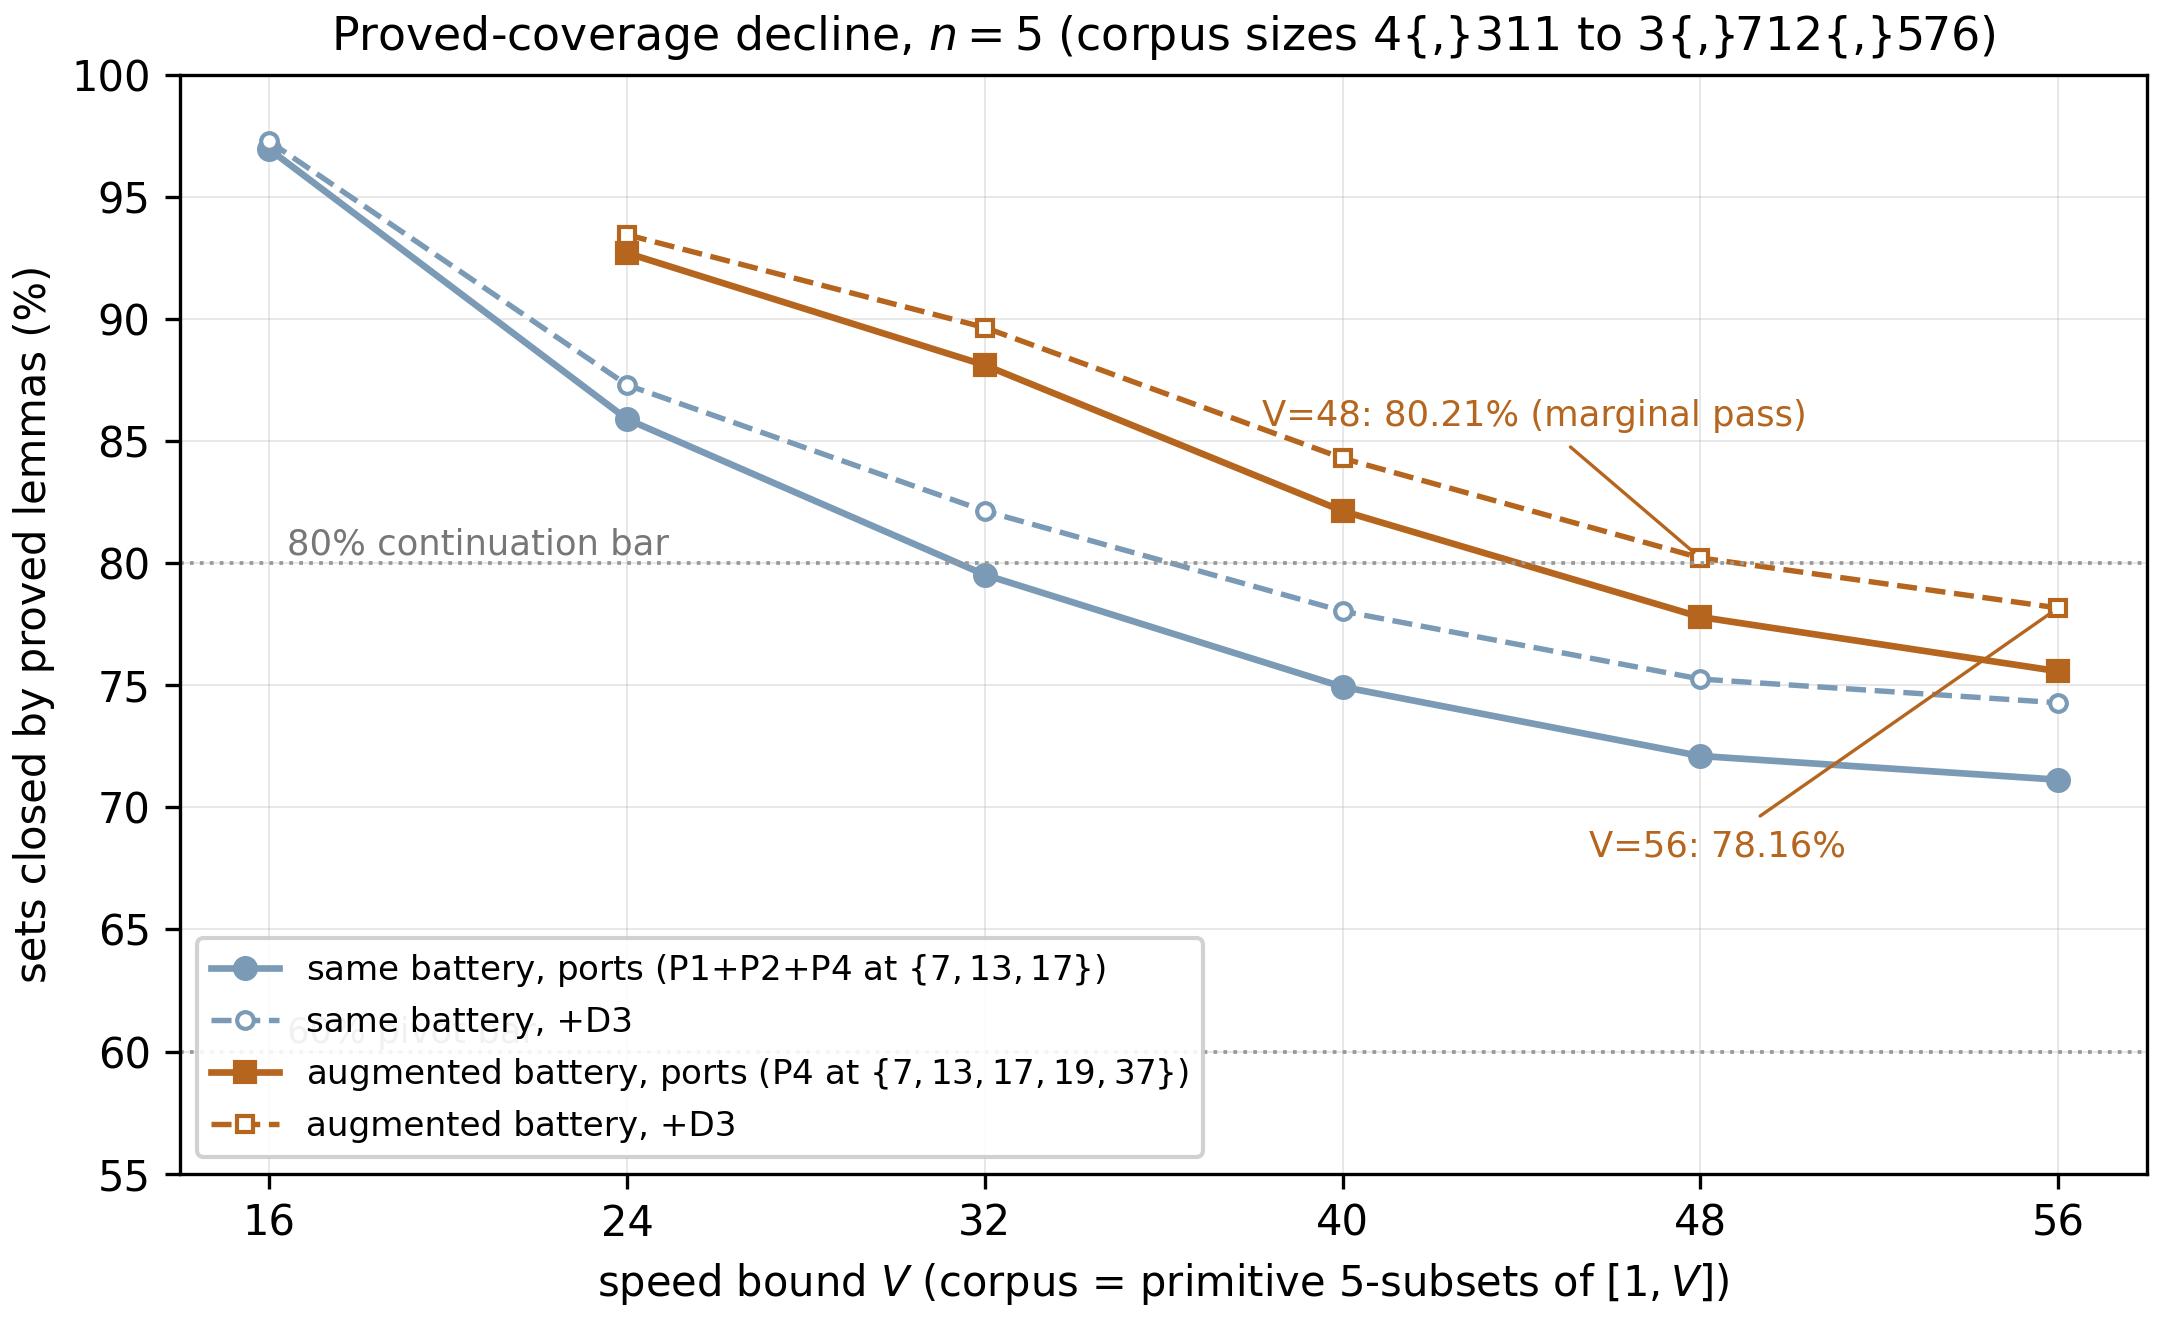
\includegraphics[max width=\textwidth, max height=0.36\textheight]
  {fig_decay.png}
\end{center}

Two framing statements, both true, must be carried together. At
\emph{matched range} ($V\le 16$, the overlap region of $4{,}311$ sets),
the reformulation performs at least as well one rung up: $96.94\%$ proved
ports at $n=5$ against $94.61\%$ at $n=4$---the strongest single datum
against the worry that the base rung closed by accident of dimension. At
\emph{growing ranges} the proved rate drops, and the drop decomposes
exactly: at $V=56$ on the same battery, the $1{,}798{,}577$ certifying
pairs that carry no proved flag split into $593{,}148$
all-invertible pairs at the then-unclassified primes $19,37$, plus
$1{,}205{,}429$ kernel-world pairs at composite moduli
($861{,}988$ at $N\le47$, $267{,}331$ at $48$--$79$, $65{,}626$ at
$80$--$95$, $10{,}484$ at $96$--$111$). After augmentation the first bucket vanishes
identifiably---the self-check ``unflagged all-invertible pair at $19$ or
$37$'' returns zero at every range---and the residual is \emph{purely}
the kernel world: mixed order signatures at composite moduli, one named
class. The classifications close a shrinking share of the verified tier
($48.4\%\to42.0\%\to28.5\%\to20.0\%\to15.1\%$ of it over $V=24\to56$) as the
incidence of $19/37$ pairs saturates; this is why the augmented curve
decays even though the rigid zone itself never grows
(\S\ref{sec:rigid}).

\subsection{The empirical pair-selection law}

The verified tier closes everything, and it does so through a striking
empirical law that deserves separate statement: \emph{at every range
measured, every single speed set has at least one certifying pair whose
$(N,\text{order signature})$ configuration is never-covering}---that is
exactly why V2 closes $100\%$. On the full $V=56$ corpus, all
$3{,}712{,}576$ sets have a certifying pair (the ground truth of
$(\mathrm{TAU}$-$_5)$ itself, now verified on every primitive $5$-set
with speeds $\le56$), the per-modulus capability and
signature-capability tables leave no set unclosed, and the hard
core---certifying pairs at \emph{capable} configurations---exists
($1{,}205{,}429$ such pairs corpus-wide, all kernel-world) but is never
load-bearing. Why a safe configuration is always available is not
understood; it is the empirical face of the pair-selection law, the
first open problem of \S\ref{sec:open}.

\subsection{Interpreting the decay curve}

The reformulation's proved coverage declines as the corpus grows, and we
report the decline in both directions---what it does not
establish, and what it does. On the augmented battery, $+D_3$ coverage
runs $93.44\%\to89.64\%\to84.29\%\to80.21\%\to78.16\%$ over
$V=24\to56$; on the same battery,
$97.26\%\to87.29\%\to82.13\%\to78.03\%\to75.25\%\to74.28\%$ from
$V=16$. In residual terms the augmented series reads
$6.56\%\to10.36\%\to15.71\%\to19.79\%\to21.84\%$, with increments
$+3.80$, $+5.36$, $+4.07$, $+2.06$ points per $8$ units of $V$: roughly
linear growth with fluctuation. Five data points cannot distinguish
asymptotic deceleration from a noisy linear trend---the last increment
being the smallest is consistent with either reading---and we fit no
trend and claim none.

What the series does establish is a level fact. The $V=48$ point stood
at $80.21\%$, a marginal pass of the program's $80\%$ continuation
threshold (by $0.21$ points); the $V=56$ point falls below it at
$78.16\%$ ($1.84$ points under, with augmented ports at $75.57\%$). The
proved coverage of the present battery did not stabilize within the
tested range, and the paper's framing follows that fact. What remains
true at every range measured: open sets are zero, per-modulus
verification closes everything, every set has a certifying pair at a
never-covering configuration, and the residual is \emph{purely} the
kernel world---after the $K_{19}$/$K_{37}$ classifications, not a single
unflagged certifying pair lives at a classified prime (the self-check
``unflagged all-invertible pair at $19$ or $37$'' returns zero at every
range, both batteries). Within the tested range the reformulation is
productive; beyond it, the proved coverage of this particular battery
decays. Closing the residual requires a kernel-world structure
theorem---the analogue for composite moduli of what the class reduction
and the $K$-classifications provide for the unit world---and that theorem
is the single open mathematical problem the reformulation now has.
Whether the decay is \emph{fundamental} (an intrinsic scaling limit of
the method) or an artifact of the missing lemma family is open
problem~6 of \S\ref{sec:open}; the honest statement is that the present
data does not decide it.

\begin{remark}[the plain regime, measured correctly]\label{rem:plain}
Two notions of ``plain'' must not be conflated. A best-pair census (does
the single highest-$\tau$ pair lack polygon structure?) put the plain
share at $73\%$ at $n=5$; the battery-relevant any-pair census (does
\emph{no} pair of the set have polygon structure?) gives
$34.3\%$ at $V=24$, $36.0\%$ at $V=48$, and $35.2\%$ at $V=56$, against
$38.3\%$ at $n=4$.
The plain share does not grow with the rung on the battery basis; and
the plain regime is not monolithic---proved lemmas beyond the polygon one
close a large part of it, and every set that needs the verified tier is
plain. The difficulty at $n=5$ lives in the plain regime, but ``there''
is a third of the corpus, not three-quarters of it.
\end{remark}

% ======================================================================
% Section 6 — Open problems
% ======================================================================

\section{Open problems}\label{sec:open}

The reformulation sharpens several questions into finite, explicit form.
We list them in what we judge to be increasing distance from the present
state of the framework.

\begin{enumerate}[leftmargin=1.7em,itemsep=4pt]

\item \textbf{The two hypotheses of Theorem~\ref{thm:SC}.} The paper's
  own frontier, and now the program's closest obligation. H1g is reduced
  to the \emph{strand census}: bound the number of arrangements and the
  phase freedom per arrangement, uniformly over the renormalization
  orbits (\S\ref{sec:scale-h1})---class-by-class work over resonance
  types, with the ratio-$2$ binary cascade the dominant first class and
  uniformity across classes itself a lemma. H2m's sharp form is the
  \emph{pair-line count}: the Lemma~\ref{lem:E} three-distance
  machinery applied to the junction draws, converting the cut law from
  hypothesis to theorem and pinning $\gamma_0$ (the chain-class bound of
  Theorem~\ref{thm:chaindilate} has the right shape with constants loose
  by orders of magnitude; the route is to count on the
  $\sum o=\mathrm{ov}$ slice). H0's route is the tangency-codimension
  argument. If all three close, Theorem~\ref{thm:SC} becomes
  unconditional and yields a uniform-in-$T$ closure of the $p^2$
  covering obstruction---hence, by the lossless equivalence, the
  conjecture at the covered rungs; the honest reading after five
  iterations of the obligation sequence (\S\ref{sec:scale-status}) is
  that the reformulation has a stubborn residual, and the theorem is
  stated so that the residual is exactly what these hypotheses name.

\item \textbf{The pair-selection law.} $(\mathrm{TAU}$-$_n)$ asserts that
  some pair certifies; the empirical law of \S\ref{sec:measure} says
  something stronger and unexplained: in every corpus measured, some pair
  certifies \emph{at a configuration that never covers}---a never-capable
  $(N,\text{order signature})$. A structural reason for the ubiquity of
  safe configurations would be the first general theorem of the program
  beyond the base lemmas, and the last ingredient needed to convert
  per-modulus verification into uniform proof on the unit side.

\item \textbf{The kernel world.} After the classifications, the entire
  residual of every corpus is one class: mixed order signatures at
  composite moduli (an order-$d$ residue contributes a bad set of size
  $N/d$, so moat counting has slack exactly there). The kernel world
  already contains the base rung's single open set,
  $V=(3,5,8,13)$, whose live pair obstruction is the covering of
  $\Z_{16}$ by the effective triple $(3,5,8)$. \emph{Post-submission
  (Remark~\ref{rem:postcomposite}):} the structure theory now exists in
  proved form --- the fibration theorem (kernel bad sets are pullbacks of
  unit bad sets at reduced moduli with the same threshold, so covering at
  composite $N$ transfers to the divisor lattice of $N$), together with
  the no-unit-assistance theorems in their provable part. The $p^2$ side
  is closed outright (the three-unit cell is empty at every prime; see
  the next item); the $pq$ side is now carried by the tensor translation
  of \S\ref{sec:pq} --- verified empty to $N\le143$ and reduced to the
  same input structure, a single unbounded input after this revision's
  discharge of Input E --- with the rigid-zone lifts the remaining open
  piece.

\item \textbf{The composite micro-cases, restated.} The original form of
  this problem --- ``no covering exists at $49$, $77$, $91$; the
  obstruction is unexplained'' --- is superseded
  (Remark~\ref{rem:postcomposite}): kernel-speed coverings exist there and
  are exactly the transferred rigid-zone configurations, and the unit
  safety of $77$ is proved. The corrected open problem is the \emph{no
  unit-assisted covering conjecture}: at $N=p^2$ and $N=pq$ with $p\ge5$,
  no covering family of at most four distinct bad sets exists in which the
  kernel subfamily does not already cover. Proved: families with at most
  two unit members (fiber-cap counting, with the sharp closed-form cap
  $2\lfloor s/6\rfloor+1+[s\equiv5\pmod6]$ for fibers of prime size $s$);
  three unit members (an inclusion--exclusion identity forced to an exact
  partition, killed by the Dirichlet floor $|A\cap\lambda A|\ge2$ on arc
  intersections); pure-unit families (reduced, via the $p$-multiples,
  to the rigid zone); and, post-submission, the entire $p^2$ side --- the
  $(1K,3U)$ cell is empty at every prime $p\ge5$ via the trichotomy
  lemmas (proved for $p\ge17$ resp.\ $p\ge31$ \emph{unconditionally}: the
  one-foot input is discharged by Lemma~\ref{lem:E}; finite-case-analyzed
  at the boundary primes; false and directly checked at $7,13$) plus the
  shear-rigidity theorem for $\pm$-colliding units
  (linear per-fiber drift against pinned covering configurations;
  verified at every prime $11\le p\le113$ with exhaustive ground truth at $p\le43$) --- and, in this revision, the $pq$ side of
  the two-unit and three-unit cells: the $(1,1,2)$ cell and both
  $(1K,3U)$ orientations are verified empty at every $N=pq\le143$ ($10$
  semiprimes, over a million family checks, margins $2$--$18$), and the
  row translation (Theorem~\ref{thm:R}) reduces their closure to the same
  remaining input, with the row census and the pinning of
  \S\ref{sec:pq-census}--\S\ref{sec:pq-verify} as the measured base.
  Open: the rigid-zone lifts, and the all-$p$ discharge of the single
  remaining named input. The boundary
  instance $N=9$ --- a genuine unit-assisted covering in exactly the
  closed $p^2$ cell shape --- shows the hypothesis $p\ge5$ is necessary.
  The named computational inputs are now precise
  objects (\S\ref{sec:gt-support}): the foot-count proposition \emph{in
  its consumed form} (the one-foot trichotomy at the two size pairs
  $(2k{+}2,2k{+}1)$ and $(2k{+}1,2k{+}1)$, viable differences confined to
  $\{2,(p-1)/2\}$) is \emph{proved} --- Lemma~\ref{lem:E}, the
  three-distance foot count, clean at every prime $p\ge31$ and
  cross-checked against the census to $p\le419$; the two-foot version is
  consumed by no current proof --- leaving the
  pinning-size lemma (relative-offset sets of at most $6$ elements with
  covering counts $28$ and $68$ independent of $p$, verified to
  $p\le113$, needed by the shear-rigidity closure, and now confirmed from
  the $pq$ side by Proposition~\ref{prop:pqpinned}) as the programme's
  single unbounded input, dischargeable not by
  bounded search but by the four-family covering classification
  (Conjecture~\ref{conj:SL}) --- which is the programme's route to an
  unconditional-in-$p$ statement.

\item \textbf{Rigid-zone termination.} Is the unit-capable set finite at
  each rung? Within the verified range (primes $\le 150$, composites
  $\le 111$) the $n=5$ zone is exactly $\{7,13,17,19,37\}$, but no
  finiteness argument is known, and the $n=4\to n=5$ transition
  ($11$ out, $\{17,19,37\}$ in) shows the zone is not monotone in the
  rung. Finiteness at one rung would make the classification program of
  \S\ref{sec:rigid} literally completable.

\item \textbf{The successor no-covering conjecture}
  (Conjecture~\ref{conj:successor}): for prime $N\ge 41$, four
  translates of $S_h$ never cover $\Z_{(N-1)/2}$. Counting never
  obstructs there ($4(2h+1)-3\ge N$), so the statement is purely
  multiplicative, the exact analogue one rung up of the $n=4$
  no-covering statement. The classifications of
  Theorems~\ref{thm:K4}--\ref{thm:K37} are the complete positive side of
  the ledger: every capable prime $\le 37$, classified.

\item \textbf{Is the decay fundamental?} The proved-coverage rate
  declines with range (\S\ref{sec:measure}): on the augmented battery
  the residual grows $6.56\%\to21.84\%$ over $V=24\to56$, with
  increments $+3.80$, $+5.36$, $+4.07$, $+2.06$ points per $8$ units of
  $V$---roughly linear growth with fluctuation, no established trend in
  either direction. The level fact is sharp: coverage fell below the
  program's $80\%$ continuation threshold at $V=56$ ($78.16\%$). The
  alternatives remain: either the decay is intrinsic to the
  reformulation (proved coverage has a range-dependent ceiling), or it
  is an artifact of the battery---specifically of the absence of a
  kernel-world lemma, since the kernel world is $100\%$ of the residual.
  Five data points do not decide the question; a kernel-world structure
  theorem would.

\item \textbf{Plain-regime growth.} On the any-pair basis the plain share
  is stable across rung and range ($38.3\%$ at $n=4$; $34.3\%$--$36.0\%$
  at $n=5$), but the verified-only sets are all plain, and the
  polygon lemma's share shrinks structurally as $T$ grows (a residue is
  polygon-certifiable only when some $j\mid N$ with $j\le T$ avoids all
  residues). Does the plain share grow with $n$, and at what rate?

\item \textbf{Higher rungs.} At $n=6$ ($T=7$, five bad sets per pair) the
  rigid zone should be denser (more translates available) and the kernel
  world larger. The program's method---run the battery, map the new
  rigid zone, generate the classifications the new level demands, replace
  the ports that die---is exactly what was executed at $n=5$; whether it
  survives a third rung is untested. \emph{Post-submission}
  (\S\ref{sec:higherrung}): the census+shear method \emph{does} survive
  the third and fourth rungs. At the critical cell of $T=8$ the fiber
  census is exactly eleven families with placement counts constant in
  $p$ (Proposition~\ref{prop:T8census}, seventeen primes); the
  $\pm$-colliding-only law holds at both rungs in the mechanism range;
  the drift law is $T$-free (Lemma~\ref{lem:rungT}); the shear step
  survives the growing pinned sets because the growth is dimensional
  (solution sets $\approx k^2$, projections saturating at $42$ against
  $|U|=(T-2)k+\epsilon-1$, exit time $\le2$); and the frontier cells are
  empty --- $(1K,4U)$ at $T=7$ for every prime $11\le p\le61$, $(2K,4U)$
  at $T=8$ for every prime $17\le p\le43$ tested. The rigid-zone lift
  itself (pure-unit families) remains open at every rung, as does the
  $T=8$ $(1K,5U)$ cell, whose five-difference census is a zoo (840
  $\pm$-distinct families at $k=2$) --- the honest boundary of the port,
  and now the object of the conditional scaling-closure attack of
  \S\ref{sec:scale}: Theorem~\ref{thm:SC} closes it under H1g and the
  H2 pair, with the strand census as the named remaining obligation.

\item \textbf{Bridges to neighboring methods.} Three external toolkits
  interface naturally with the reformulation's finite statements.
  (a)~The covering lemmas now have a \emph{proved} bridge: the group-ring
  translation (\S\ref{sec:groupring}) turns them into sign conditions on
  a sparse identity in $\Z[\Z_p]$, proved as Theorem~\ref{thm:GT} and
  machine-verified on every covering in the $p\le61$ census; its census
  law (four difference families with $p$-independent placement counts,
  Conjecture~\ref{conj:SL}) is the object the remaining two lemmas must
  prove, and it sits precisely in the Lam--Leung--de~Bruijn--Schoenberg
  theory of sparse cyclotomic divisibility.
  (b)~The no-covering
  statements (Conjecture~\ref{conj:successor} and its $n=4$ ancestor)
  concern coverings of cyclic groups by \emph{multiplicative
  arcs}---images of intervals under multiplication. Additive-combinatorial
  covering theory (Kneser-type theorems, Cauchy--Davenport and weighted
  variants) is the classical toolkit for covering questions in $\Z_N$;
  whether any of its forms applies to multiplicative arcs is open, and a
  positive answer at prime $N$ would settle the successor conjecture.
  (c)~Covering-radius problems for lattice zonotopes are governed
  matroidally, and log-concave polynomial methods have turned matroidal
  counting statements into general theorems (Mason's ultra-log-concavity
  conjecture being the template); whether the pair-sum covering problems
  admit a zonotope--matroid encoding whose associated polynomial has a
  stability property is the corresponding question here---if they do, the
  kernel world would be its near-equality cases, and the sign-mixed
  sparse divisibility of \S\ref{sec:gt-outlook} is the natural first
  candidate. The first bridge is exploited; the other two are recorded as
  directions, not claims. \emph{Post-submission} (final revision): the
  third bridge was subsequently engaged as a full strand and is now
  closed. The zonotope--Ehrhart encoding exists---the Lonely-Runner
  zonotope of the instance at denominator $N$, its dilate family
  $mZ(V)$---and its arithmetic is entirely stable: the $h^*$-polynomials
  of both canonical families (the harmonic instances $v=(1,\dots,n)$ and
  the rung-$2$ instances $v=(1,\dots,n{-}1,2n)$) are real-rooted,
  log-concave, and Newton at every $n\le 10$, verified in exact
  rational arithmetic at $45$ digits \cite{companion-paper}. The
  geometric control the bridge asked for, however, is false in its
  natural form: the deepest-hole reading---the covering optimum
  attained at the zonotope's center, $\rho=\delta$---fails from $n=5$
  onward with exact rational witnesses (at the harmonic $n=5$ instance
  $m=5$, $\rho\ge 4183/12288>\tfrac13$, improved twice---from
  $97/288$ to $607/1792$ by the first certification session's
  follow-up and to $4183/12288$ by the companion paper's external
  audit), the modular law that would
  govern it (deepest hole at the center exactly when $n\mid m$) breaks
  at $n=5$ (the odd multiples $5$ and $15$ fail exactly; the even and
  higher multiples $10,20,25,30$ are certified, $m=10$ closing with
  the companion paper's third revision) and is extinct at $n=6$, and
  the strictness of $h^*$ neither
  tracks nor predicts the covering gap (rank correlation at the noise
  level). The bridge's question is thus answered in the negative for
  the natural encoding, and with the same shape as the internal
  program's boundary: arithmetic fidelity, no margin. The witnesses,
  the exact certification ladder, and the $h^*$ addendum are the
  subject of the companion paper \cite{companion-paper}.
\end{enumerate}

% ======================================================================
% Section 7 — Reproducibility and soundness record
% ======================================================================

\section{Reproducibility and soundness record}\label{sec:sound}

Every empirical and classification claim in this paper rests on exact
integer computation, and every computation is paired with a control or an
independent reimplementation. This section records the checks; the
committed scripts, logs, and experiment notes are bundled with the paper
\cite{prog-artifacts}. The record matters beyond convention here: a
measurement program on $10^6$-scale corpora is exactly the setting where
silent bugs masquerade as findings, and the discipline below is what
separates the two.

\begingroup
\footnotesize
\setlength{\LTcapwidth}{\textwidth}
\begin{longtable}{@{}p{3.7cm}>{\raggedright\arraybackslash}p{8.2cm}>{\raggedright\arraybackslash}p{3.1cm}@{}}
\caption{The verification record. All counts are of exact checks with the
stated outcome; ``0 mismatches'' means exact agreement of two independent
computations.}\label{tab:sound}\\
\toprule
check & scope & outcome \\
\midrule
\endfirsthead
\multicolumn{3}{l}{\footnotesize Table~\ref{tab:sound} (continued)}\\
\toprule
check & scope & outcome \\
\midrule
\endhead
\bottomrule
\endfoot
\bottomrule
\endlastfoot
size law (Lem.~\ref{lem:size}) & all residues, $N\le111$ ($T{=}6$),
  $N\le31$ ($T{=}5$) & 0 violations \\
classification predicate $\iff$ mask covering & exhaustive over unit
  multisets at $7,11,13,17,19,37$ ($126$--$82{,}251$ per modulus) &
  0 mismatches \\
$K_{19}$/$K_{37}$ class list $\iff$ covering & all unit
  $4$-multisets, both directions ($5{,}985$ and $82{,}251$) &
  0 mismatches \\
battery soundness (flag $\Rightarrow$ certify) & exhaustive
  $N\le31$ ($46{,}371$ at $n{=}4$; $324{,}626$ at $n{=}5$);
  exhaustive $N\in\{37,49,81,95\}$ ($91{,}390$; $270{,}725$;
  $1{,}929{,}501$; $3{,}612{,}280$); exhaustive $N\in\{99,111\}$
  ($4{,}249{,}575$; $6{,}672{,}876$); random $32$--$95$ ($256{,}000$);
  random $96$--$111$ ($64{,}000$) &
  0 violations \\
polygon constructive witness & sampled across all corpora & 0 failures \\
reduced-optimum cross-check & direct grid maximization vs.\ bitmask,
  sampled & 0 mismatches \\
lift law (Lem.~\ref{lem:lift}) & random lifts & 0/2{,}727 \\
equality theorem (Thm.~\ref{thm:equality}) & fresh non-circular check
  (folklore breakpoints vs.\ pair lattices), $885/885$; from-scratch
  independent reimplementation (time domain, differences included,
  $n=2$--$6$, $v\le200$), with exact anchors & $2{,}870/2{,}870$ \\
ground truth of $(\mathrm{TAU}$-$_5)$ & every primitive $5$-set,
  $v\le56$ & $3{,}712{,}576/3{,}712{,}576$ \\
trichotomy proof, line by line & every intermediate claim of Lemma~T
  (non-wrapping, span bounds, two-lattice descent, two-block identity)
  at all primes $p\le250$, plus the run lemmas at $p\le37$ & 0 violations \\
colliding-unit ground truth & all $\pm$-colliding $(1K,3U)$ families,
  both collision topologies, $p\le43$ & $3{,}3$\,M families, 0 coverings \\
shear linearity & per-fiber $t$-space offsets of colliding lifts,
  all $v_2,m,j$ at $p\le37$ & 0 violations of $\sigma_3-\sigma_2=-\bar u mj$ \\
boundary finite case analyses & Lemma~B at $11$; Lemma~A at $19$: every
  viable configuration certified, independent brute force in
  agreement (and reproducing the known failures $50$ at $7$, $2$ at $13$
  as witness-tuple counts; the $17,31,37$ analyses of the earlier draft
  are now redundant with the extended proof ranges) & exact \\
group-ring identity (Thm.~\ref{thm:GT}) & $36{,}308$ checks: all $52$
  Lemma~A exceptions ($E$-profiles exactly as classified), every covering
  of the $15$-prime census ($12{,}256$), $24{,}000$ random configurations
  incl.\ non-coverings (sharp signed form; sign~$\Leftrightarrow$~covering;
  kernel~$=\Z\overline\Phi_p$) & all pass \\
covering census (Prop.~\ref{prop:census}) & all critical coverings over
  all $(d_2,d_3)\in(\Z_p^*)^2$, normal form, $p\in\{5,7,11,13,17,19,23,29,31,37,41,43,47,53,59,61\}$
  & four families, counts constant in $p$; $0$ $\pm$-distinct coverings at
  $p\ge11$ \\
foot census (Input E) & every prime $p\le419$, both classes, every
  critical $(s_1,s)$, $\pm$-reps $d\ge2$: one/two-foot viable sets;
  the M4/M5 consumed pairs; Lemma B's contained census at $(6,6)$ &
  consumed form clean from $p\ge31$; now \emph{proved}
  (Lemma~\ref{lem:E}) \\
Lemma E machinery (Lemmas~\ref{lem:E0}--\ref{lem:E}) & every $(p,d,s)$
  with $p\le500$ ($45$ primes, $10{,}410$ triples): column decomposition,
  band and block identities, the pair-sum identity as an \emph{exact}
  equality, the auxiliary bounds; the theorem direct to $p\le2000$
  ($136{,}806$) and, via the identity, to $p\le4000$ ($367{,}986$);
  endpoint/dirty-prime values exact; $76$/$76$ viable-set agreement with
  the foot census & all hold \\
parity mechanism (Prop.~\ref{prop:pindep}) & every census $(2,2)$ solution
  at $p\in\{23,29,41,31,37,43\}$: integer-parity runs, non-wrapping,
  spills $\le\mathrm{ov}$ in $A_1$; per-(multiset, family) counts &
  $100\%$; counts $=$ Table~\ref{tab:permultiset} \\
$pq$ translation (Thm.~\ref{thm:R}) & constants; footprint formula
  ($4{,}394$ set equalities, $8$ moduli); row census ($24$ resp.\ $312$,
  $14$ primes); $(1,1,2)$ cells ($143{,}733$ checks, $10$ moduli);
  $(1K,3U)$ cells ($989{,}000$ checks); pinning ($37{,}672$ rows,
  $\le6$ good rows); $T$-10 reproduction at $77,91$ &
  all pass; $0$ coverings \\
higher-rung machinery (Lem.~\ref{lem:rungT}) & three-tier arc law vs the
  committed $T=6$ tables ($p\le37$, both classes) and at $19$ primes of
  $T=7/T=8$ (all residue classes, every $a_0$); footprint formula vs
  direct $Z_{p^2}$ enumeration; drift identity at $T\in\{7,8\}$ &
  $957/957$; $3{,}528/3{,}528$ \\
$T=8$-critical census (Prop.~\ref{prop:T8census}) & $17$ primes, all four
  odd $\epsilon$ classes, $k\le17$: exactly $11$ families, counts
  $288$ ($\epsilon\in\{3,7\}$) resp.\ $2{,}784$ ($\epsilon\in\{1,5\}$)
  constant in $p$; $0$ $\pm$-distinct in the mechanism range & exact \\
$T=7$ census (Prop.~\ref{prop:T7census}) & $18$ primes, all six
  $\epsilon$ classes, $k\le11$: core-eleven dominance ($\approx90\%$ at
  $k\ge6$), tail decay $183\to43$, $0$ $\pm$-distinct at $k\ge4$/$k\ge2$ &
  exact \\
higher-rung cells (Prop.~\ref{prop:shearT78}) & $(1K,4U)$ at $T=7$:
  census-restricted ground truth (distinctness-filtered) at every prime
  $11\le p\le61$ --- $0$ coverings, best exit $2$; brute-force control at
  $p\in\{5,7,11\}$ agreeing exactly at the degenerate $p=5$ ($8$
  coverings both ways); $(2K,4U)$ at $T=8$ at $17\le p\le43$ --- $0$
  coverings; sampled controls $20$K families at four primes & exact \\
\midrule
$n=4$ control & full record incl.\ the open set $=(3,5,8,13)$ &
  exact \\
range controls, both batteries & $V=16/24/32/40/48$, all tiers, unflagged
  pair totals and decompositions & exact vs.\ committed logs \\
capability controls & zones, counts $20/68/16/64/32$, safety of
  $48$--$111$ & exact \\
independent capability recounts & set-based scanner at all danger moduli
  ($27$ moduli) & exact agreement \\
\end{longtable}
\endgroup

\subsection{Controls}

Every experiment run begins with hard assertions against previously
committed numbers before any new number is produced: the $n=4$ corpus
reproduces the committed record (including the identity of the open
set); the $n=5$ corpora at $V=16,24,32,40,48$ reproduce every committed
tier count for both batteries, the corpus-wide unflagged-pair totals and
decompositions included; the capability scan reproduces the committed
zones, the per-modulus covering counts, and the safety of $48$--$111$ (the
composite range extended twice, both times with the new moduli re-derived
by the independent set-based scanner); and the signature-capability maps
for $48$--$79$ and $80$--$95$ match the committed dictionaries exactly. The classifications were additionally anchored by hand: the
$\Z_{17}$ covering of Example~\ref{ex:17} was expanded by hand, the
$D_3$ falsifier $(1,1,2,3)$ on $\Z_7$ and its exclusion
$N\equiv1\pmod6$ were checked by hand, and the $K_{19}$/$K_{37}$
covering counts were reproduced by three independent implementations
(bitmask, frozenset, exponent-space).

\subsection{The cross-validation discipline}

The program's standing rule is that every empirical claim must be checked
against committed data or a reference implementation before being cited.
The rule earned its keep: across the program's lifetime it caught, before
any affected number was recorded, a divisibility test written as a
bitwise OR; a sampling artifact in which a $720$-point time grid silently
missed denominators like $11$ and briefly masqueraded as counterexamples
to the equality theorem; an unsound counting bound for mixed-order
residues ($245$ flagged-but-non-certifying pairs, all caught by the
flag-implies-certify sweep); an off-by-one in the capability scanner that
contradicted the committed $n=4$ zone; a flag-parsing slip; a
verified-tier flag leaking into a proved tier (caught by a too-good
``$100\%$''); a diagnostic accumulating corpus-wide instead of
per-tier (caught by an impossible count); a mislabeled canonicalization
of cyclic translate classes (contains-$0$ representatives are not orbit
representatives on $\Z_m$); and an unsound attempt to quotient the
classification by negation ($B_{-w}=B_w$, so negation is not a symmetry);
an off-by-one in the minimal-arc length of the census fit test (caught by
the assertion that every enumerated covering has $E\ge0$, fixed, and then
confirmed against a no-prune brute force); and a count-semantics
reconciliation forced by the census run (the earlier $50$/$2$ at
$p=7$/$13$ are witness-tuple counts, one per $(d_2,d_3,a_2)$ with a
completing placement, while the true solution counts are $272$
normalized configurations $=$ $68$ set-triples and $8$ $=$ $2$ --- the
brute force confirms both readings, and the identity check ran on the full
solution set).
Each fix was verified by the control that caught it. We report these not
as penance but as evidence that the numbers above survived an adversarial
process.

\subsection{Artifacts}

\begingroup\sloppy
The bundle \cite{prog-artifacts} contains the equality-theorem
verifications (\texttt{V1\_equality\_fresh\_check.py} and the
from-scratch \texttt{EQ\_independent\_verify.py}); the independent
capability cross-checks (\texttt{N5\_prime\_scan\_crosscheck.py} and the
set-based scanners); the literature-search scripts and raw results; the
experiment notes summarizing each stage; and the corpus and battery
engines with their controls, one per stability extension, each with its
full run log:
\begin{itemize}[leftmargin=2.2em,itemsep=1pt,topsep=2pt]
  \item \texttt{N5\_leverage\_experiment.py} (the committed $n=5$
        battery and rigid-zone scan),
  \item \texttt{N6\_stability\_experiment.py} (the $V=32/40$ extension
        and the composite capability completion to $N\le79$),
  \item \texttt{N7\_classify\_19\_37.py} (the $K_{19}$/$K_{37}$
        classifications and the augmented re-measurement),
  \item \texttt{N8\_v48\_extension.py} (the $V=48$ data point, both
        batteries, capability to $N\le95$),
  \item \texttt{N9\_v56\_extension.py} (the $V=56$ data point, both
        batteries, capability to $N\le111$; staged execution with
        per-stage state persistence and hard controls re-asserted at
        every stage),
  \item \texttt{ap\_lemmas\_verify.py} (the trichotomy/Lemma~A/B
        verification of the companion note: exact lemma search,
        censuses, capacity structure, cell anchors; $p\le250$),
  \item \texttt{trichotomy\_linecheck.py} (the line-by-line machine
        check of the trichotomy proof, including the general-arc
        variant),
  \item \texttt{pm\_colliding\_close.py} (the $\pm$-colliding closure:
        ground truth, fiber structure, shear linearity, pinning tables,
        pigeonhole),
  \item \texttt{boundary\_finite\_cases.py} (the boundary-prime finite
        case analyses with margin certificates and the independent
        brute-force cross-check),
  \item \texttt{groupring\_bridge.py} (the group-ring translation
        verification: identity checks on all exceptions and census
        coverings, sharp-form sampling, kernel checks, the four-family
        census with per-multiset counts, defect statistics, and the
        witness/solution count reconciliation; output
        \texttt{out\_groupring\_bridge.json}, log
        \texttt{groupring\_run.log}),
  \item \texttt{foot\_census.py} (the Input~E boundary census: one/two-foot
        viable sets at every prime $p\le419$, the consumed-pair
        cleanliness, and the Lemma~B $p=17$ form check; output
        \texttt{out\_foot\_census.json}),
  \item \texttt{lemmaE\_master.py} (the three-distance foot-count
        verification, discharging Input~E: column decomposition, band and
        block identities, the pair-sum identity as an exact equality, the
        auxiliary bounds of Lemma~\ref{lem:E4}, the theorem of
        Lemma~\ref{lem:E} direct to $p\le2000$ and via the identity to
        $p\le4000$, the endpoint and dirty-prime values of
        Remark~\ref{rem:Esharp}, and the viable-set cross-check against
        the foot census; output \texttt{out\_lemmaE.json}),
  \item \texttt{pq\_side.py} / \texttt{pq\_side2.py} / \texttt{parity\_check.py}
        (the $pq$ translation battery: constants and footprint formula,
        row censuses, $(1,1,2)$ and $(1K,3U)$ cell enumeration with
        margins, pinning and drift analysis, and the parity-mechanism
        structural check; outputs \texttt{out\_pq\_side.json},
        \texttt{out\_pq\_side2.json}),
  \item \texttt{higher\_rung\_step1.py} with the resumable
        \texttt{drive\_step1.py} (the general-$T$ machinery controls and
        the higher-rung censuses: the $T=7$ four-difference census at
        $18$ primes with per-family projections, the $T=8$-critical
        census at $17$ primes, the $T=8$ five-difference probe; output
        \texttt{out\_higher\_rung\_step1.json}, log
        \texttt{higher\_rung\_run1.log}),
  \item \texttt{higher\_rung\_step2.py} (the shear side at the higher
        rungs: the drift-law verification, the census-restricted and
        brute-force ground truths for the $(1K,4U)$ cell at $T=7$ and the
        $(2K,4U)$ cell at $T=8$, the exit-time measurements; output
        \texttt{out\_higher\_rung\_step2.json}),
  \item \texttt{higher\_rung\_step3.py} (the sampled family controls for
        the two frontier cells; output
        \texttt{out\_higher\_rung\_step3.json}),
  \item \texttt{pool\_sat.c} with \texttt{gt\_pool\_brute.py} (the pool
        saturation censuses of \S\ref{sec:scale-pool}: the $m$-general
        admissibility checker in two cross-validated implementations
        plus dump/resume stride sampling, and the independent
        pure-enumeration brute force agreeing on $21/21$ sampled tuples
        across $p=17/19/23/31$; dumps
        \texttt{dump\_p\{17,19,23\}.tsv}, \texttt{pool\_T8\_p31.tsv},
        \texttt{dump\_T9\_p\{29,31\}\_sample.tsv}),
  \item \texttt{h2\_pair\_check.py} (the zone-resolved cut-quality
        measurement of Table~\ref{tab:gamma}: per-pair $\gamma$ on the
        committed cells, $764$ pairs; output
        \texttt{out\_h2\_pair\_check.json}),
  \item \texttt{chain\_structure\_check.py} (the chain-class machine
        checks of Lemmas~\ref{lem:overlapsum}--\ref{lem:chainbox} and
        Theorem~\ref{thm:chaindilate}: $123{,}240$ solutions, the sum
        identity, the reach bound, and the count reconciliations),
  \item \texttt{scaling\_closure\_extract.py} and
        \texttt{scaling\_closure\_verify.py} (the read-only calibration
        from the committed JSONs and the targeted lemma verification of
        \S\ref{sec:scale-cut}: solution-volume probes, two-fiber dilate
        law, resonance zones, cascade depths at the committed cells,
        sign robustness; outputs
        \texttt{out\_scaling\_closure\_extract.json},
        \texttt{out\_scaling\_closure\_verify.json}),
  \item \texttt{h1\_t8\_census.py}, \texttt{h1\_t8\_structure.py},
        \texttt{h1\_t8\_prime.py}, \texttt{h1\_t8\_path.py} (the
        $T=8$ volume census, mechanism probes, and prime extensions of
        \S\ref{sec:scale-h1}, with the independent brute-force ground
        truth ($9/9$ keys) and the renormalization-orbit verification;
        states \texttt{h1\_t8\_state.json} /
        \texttt{h1\_t8\_prime\_state.json}, outputs
        \texttt{out\_h1\_t8\_census.json},
        \texttt{out\_h1\_t8\_structure.json},
        \texttt{out\_h1\_t8\_prime.json}).
\end{itemize}
All runs are deterministic; every number in
\S\ref{sec:measure}--\ref{sec:sound} appears verbatim in a committed log.
\endgroup

\subsection{Data and code availability}

The complete artifact bundle (scripts, committed logs, JSON records, and
the figures) accompanies this paper and is deposited for public access
together with the PDF; the sources build with \texttt{tectonic} and a
single command. The verification scripts have no dependencies beyond
CPython~3.12 with \texttt{numpy}; each re-derives its controls from
first principles and asserts them before producing any new number, so
any single experiment can be re-audited in isolation. This document, its
companion notes, and the bundle are released under the Creative Commons
Attribution 4.0 license (CC~BY~4.0), the better to allow the community
to re-run, refute, or extend the record.


% ======================================================================
% Bibliography (manual, ordered by first citation)
% ======================================================================

\begingroup\sloppy\raggedright
\begin{thebibliography}{17}

\bibitem{PS-survey}
G.~Perarnau and O.~Serra,
\emph{The Lonely Runner Conjecture turns 60},
arXiv:2409.20160 (survey).

\bibitem{Wills}
J.~M. Wills,
\emph{Zwei S\"atze \"uber inhomogene diophantische Approximation von
Irrationalzahlen},
Monatsh.\ Math.\ 71 (1967).

\bibitem{Cusick1973}
T.~W. Cusick,
\emph{View-obstruction problems},
Aequationes Math.\ \textbf{9} (1973), 165--170.

\bibitem{Rosenfeld8}
M.~Rosenfeld,
\emph{The lonely runner conjecture holds for eight runners},
arXiv:2509.14111 (2025).

\bibitem{Trakulthongchai}
T.~Trakulthongchai,
\emph{Nine and ten lonely runners},
arXiv:2511.22427 (2025).

\bibitem{Sungkawichai}
T.~Sungkawichai and T.~Trakulthongchai,
\emph{Eleven, twelve, and thirteen lonely runners},
arXiv:2604.23906 (2026).

\bibitem{Allikvere}
J.~Allikvere,
\emph{Fourteen and fifteen lonely runners},
arXiv:2609.02604 (2026).

\bibitem{MSS}
R.~D. Malikiosis, F.~Santos, and M.~Schymura,
\emph{Linearly-exponential checking is enough for the Lonely Runner
Conjecture and some of its variants},
arXiv:2411.06903 (2024).

\bibitem{Kravitz}
N.~Kravitz,
\emph{Barely lonely runners and very lonely runners},
arXiv:1912.06034 (2019).

\bibitem{FanSun}
H.~T. Fan and A.~Sun,
\emph{Amending the Lonely Runner Spectrum Conjecture},
arXiv:2306.10417 (2023).

\bibitem{GiriKravitz}
V.~Giri and N.~Kravitz,
\emph{The structure of Lonely Runner spectra},
arXiv:2304.01462 (2023).

\bibitem{Cordella}
F.~Cordella,
\emph{Odd denominators in the Lonely Runner spectrum for six speeds},
arXiv:2609.03444 (2026).

\bibitem{Zhang}
Y.~Zhang,
\emph{Tight instances of the Lonely Runner Conjecture: complete
classification of one-entry modifications, a new infinite family, and the
growth bound},
arXiv:2608.13599 (2026).

\bibitem{BeckEverett}
M.~Beck and S.~Everett,
\emph{Lonely Runner Relations},
arXiv:2609.06259 (2026).

\bibitem{Rifford}
L.~Rifford,
\emph{On the time for a runner to get lonely},
arXiv:2111.13688 (2021).

\bibitem{Tao-blog}
T.~Tao,
\emph{A remark on the lonely runner conjecture},
weblog post, 13 May 2015; the observation that the optimal time is
rational with denominator the sum or difference of two speeds appears
in the comments.
\\[2pt]
\url{https://terrytao.wordpress.com/2015/05/13/}\\
\url{a-remark-on-the-lonely-runner-conjecture}

\bibitem{prog-artifacts}
LRC reformulation program,
\emph{Committed scripts, run logs, and experiment notes},
unpublished artifact bundle accompanying this paper (2026).

\bibitem{MirskyNewman}
L.~Mirsky and D.~J.~Newman,
unpublished (the distinct-moduli theorem for exact covering systems);
see the account in
H.~Davenport and R.~Rado,
\emph{Covering systems of negative congruences},
J.\ London Math.\ Soc.\ \textbf{38} (1963), 509--516.

\bibitem{deBruijnSchoenberg}
The classical structure theorem for vanishing sums of roots of unity
with nonnegative rational coefficients (R\'edei, de~Bruijn, and
I.~J.~Schoenberg, independently, 1950s); see the account and
bibliography in \cite{LamLeung}.

\bibitem{LamLeung}
T.~Y.~Lam and K.~H.~Leung,
\emph{On the cyclotomic polynomial $\Phi_{pq}(X)$},
Amer.\ Math.\ Monthly \textbf{103} (1996), 562--564; and
\emph{On vanishing sums of roots of unity},
J.\ Algebra \textbf{224} (2000), 91--109.

\bibitem{BrandenHuh}
P.~Br\"anden and J.~Huh,
\emph{Lorentzian polynomials},
Ann.\ of Math.\ (2) \textbf{192} (2020), no.~3, 821--915.

\bibitem{companion-paper}
Companion paper (this program),
\emph{Every natural strengthening is false: type mismatch in lossless
reformulations of the Lonely Runner Conjecture},
with the witness archive, the exact certification ladder, and the
$h^*$ addendum through $n=10$.

\end{thebibliography}
\endgroup


\end{document}
